% A LaTeX template for ARTICLE version of the MSc Thesis submissions to 
% Politecnico di Milano (PoliMi) - School of Industrial and Information Engineering
%
% S. Bonetti, A. Gruttadauria, G. Mescolini, A. Zingaro
% e-mail: template-tesi-ingind@polimi.it
%
% Last Revision: October 2021
%
% Copyright 2021 Politecnico di Milano, Italy. Inc. NC-BY

\documentclass[11pt,a4paper]{article} 

%------------------------------------------------------------------------------
%	REQUIRED PACKAGES AND  CONFIGURATIONS
%------------------------------------------------------------------------------
% PACKAGES FOR TITLES
\usepackage{titlesec}
\usepackage{color}

% PACKAGES FOR LANGUAGE AND FONT
\usepackage[utf8]{inputenc}
\usepackage[english]{babel}
\usepackage[T1]{fontenc} % Font encoding

% PACKAGES FOR IMAGES
\usepackage{graphicx}
\graphicspath{{Images/}}
\usepackage{eso-pic} % For the background picture on the title page
\usepackage{subfig} % Numbered and caption subfigures using \subfloat
\usepackage{caption} % Coloured captions
\usepackage{transparent}

% STANDARD MATH PACKAGES
\usepackage{amsmath}
\usepackage{amsthm}
\usepackage{bm}
\usepackage[overload]{empheq}  % For braced-style systems of equations

% PACKAGES FOR TABLES
\usepackage{tabularx}
\usepackage{longtable} % tables that can span several pages
\usepackage{colortbl}

% PACKAGES FOR ALGORITHMS (PSEUDO-CODE)
\usepackage{algorithm}
\usepackage{algorithmic}

% PACKAGES FOR REFERENCES & BIBLIOGRAPHY
\usepackage[colorlinks=true,linkcolor=black,anchorcolor=black,citecolor=black,filecolor=black,menucolor=black,runcolor=black,urlcolor=black]{hyperref} % Adds clickable links at references
\usepackage{cleveref}
\usepackage[square, numbers, sort&compress]{natbib} % Square brackets, citing references with numbers, citations sorted by appearance in the text and compressed
\bibliographystyle{plain} % You may use a different style adapted to your field


% PACKAGES FOR THE APPENDIX
\usepackage{appendix}

% PACKAGES FOR ITEMIZE & ENUMERATES 
\usepackage[inline]{enumitem}

% OTHER PACKAGES
\usepackage{amsthm,thmtools,xcolor} % Coloured "Theorem"
\usepackage{comment} % Comment part of code
\usepackage{fancyhdr} % Fancy headers and footers
\usepackage{lipsum} % Insert dummy text
\usepackage{tcolorbox} % Create coloured boxes (e.g. the one for the key-words)

%-------------------------------------------------------------------------
%	NEW COMMANDS DEFINED
%-------------------------------------------------------------------------
% EXAMPLES OF NEW COMMANDS -> here you see how to define new commands
\newcommand{\bea}{\begin{eqnarray}} % Shortcut for equation arrays
\newcommand{\eea}{\end{eqnarray}}
\newcommand{\e}[1]{\times 10^{#1}}  % Powers of 10 notation
\newcommand{\mathbbm}[1]{\text{\usefont{U}{bbm}{m}{n}#1}} % From mathbbm.sty
\newcommand{\pdev}[2]{\frac{\partial#1}{\partial#2}}
% NB: you can also override some existing commands with the keyword \renewcommand
\newlist{inlinelist}{enumerate*}{1}
\setlist[inlinelist]{label=(\arabic*)}
\newcommand{\parspace}{\vspace{7pt}}
% \newcommand{\multirowcell}{\begin{tabular}[c]{@{}l@{}}
%----------------------------------------------------------------------------
%	ADD YOUR PACKAGES (be careful of package interaction)
%----------------------------------------------------------------------------
\usepackage{xurl}
\usepackage{subfiles}
\usepackage{siunitx}
\usepackage{csquotes}
\usepackage{svg}
\usepackage{tikz}
\usepackage{listings}
\usepackage{gensymb}


%----------------------------------------------------------------------------
%	ADD YOUR DEFINITIONS AND COMMANDS (be careful of existing commands)
%----------------------------------------------------------------------------
\def\UrlBreaks{\do\/\do-}
\usetikzlibrary{positioning,arrows.meta,shapes}


% Do not change Configuration_files/config.tex file unless you really know what you are doing. 
% This file ends the configuration procedures (e.g. customizing commands, definition of new commands)
% Configuration package
\usepackage[bottom=2.0cm,top=2.0cm,left=2.0cm,right=2.0cm]{geometry}
\raggedbottom 

% Create color bluePoli (-> manuale grafica coordinata:  https://www.polimi.it/fileadmin/user_upload/il_Politecnico/grafica-coordinata/2015_05_11_46xy_manuale_grafica_coordinata.pdf)
\definecolor{bluePoli}{cmyk}{0.4,0.1,0,0.4}

% Custom theorem environments
\declaretheoremstyle[
  headfont=\color{bluePoli}\normalfont\bfseries,
  bodyfont=\color{black}\normalfont\itshape,
]{colored}

\captionsetup[figure]{labelfont={color=bluePoli}} % Set colour of the captions
\captionsetup[table]{labelfont={color=bluePoli}} % Set colour of the captions
\captionsetup[algorithm]{labelfont={color=bluePoli}} % Set colour of the captions

\theoremstyle{colored}
\newtheorem{theorem}{Theorem}[section]
\newtheorem{proposition}{Proposition}[section]

% Enhances the features of the standard "table" and "tabular" environments.
\newcommand\T{\rule{0pt}{2.6ex}}
\newcommand\B{\rule[-1.2ex]{0pt}{0pt}}

% Algorithm description
\newcounter{algsubstate}
\renewcommand{\thealgsubstate}{\alph{algsubstate}}
\newenvironment{algsubstates}{
    \setcounter{algsubstate}{0}%
    \renewcommand{\STATE}{%
    \stepcounter{algsubstate}%
    \Statex {\small\thealgsubstate:}\space}
    }{}
    
% Custom theorem environment
\newcolumntype{L}[1]{>{\raggedright\let\newline\\\arraybackslash\hspace{0pt}}m{#1}}
\newcolumntype{C}[1]{>{\centering\let\newline\\\arraybackslash\hspace{0pt}}m{#1}}
\newcolumntype{R}[1]{>{\raggedleft\let\newline\\\arraybackslash\hspace{0pt}}m{#1}}

% Custom itemize environment
\setlist[itemize,1]{label=$\bullet$}
\setlist[itemize,2]{label=$\circ$}
\setlist[itemize,3]{label=$-$}
\setlist{nosep}

% Create command for background pic
\newcommand\BackgroundPic{% Adding background picture
	\put(237,365){
	    \parbox[b][\paperheight]{\paperwidth}{%
	    \vfill
		\centering
		\transparent{0.4}
		
\includegraphics[width=0.44\paperwidth]{raggiera_polimi.eps}%
		\vfill}
		}
}

% Set indentation
\setlength\parindent{0pt}

% Custom title commands
\titleformat{\section}
{\color{bluePoli}\normalfont\Large\bfseries}
{\color{bluePoli}\thesection.}{1em}{}
\titlespacing*{\section}
{0pt}{3.3ex}{3.3ex}

\titleformat{\subsection}
{\color{bluePoli}\normalfont\large\bfseries}
{\color{bluePoli}\thesubsection.}{1em}{}
\titlespacing*{\subsection}
{0pt}{3.3ex}{3.3ex}

% Custom headers and footers
\pagestyle{fancy}
\fancyhf{}
      
\fancyfoot{}
\fancyfoot[C]{\thepage} % page
\renewcommand{\headrulewidth}{0mm} % headrule width
\renewcommand{\footrulewidth}{0mm} % footrule width

\makeatletter
\patchcmd{\headrule}{\hrule}{\color{black}\hrule}{}{} % headrule
\patchcmd{\footrule}{\hrule}{\color{black}\hrule}{}{} % footrule
\makeatother

% Insert here the info that will be displayed into your Title page 
% -> title of your work
\renewcommand{\title}{Why can you kill mosquitoes in the dark? \\
    \large Towards solving sound localization with a biologically plausible spiking neural \\ simulation}

% -> author name and surname
\renewcommand{\author}{Paolo Marzolo}
% -> MSc course
\newcommand{\course}{Computer Science and Engineering - Ingegneria Informatica}
% -> advisor name and surname
\newcommand{\advisor}{Prof. Alberto Antonietti}
% IF AND ONLY IF you need to modify the co-supervisors you also have to modify the file Configuration_files/title_page.tex (ONLY where it is marked)
\newcommand{\firstcoadvisor}{Eng. Francesco De Santis} % insert if any otherwise comment
\newcommand{\secondcoadvisor}{} % insert if any otherwise comment

% -> author ID
\newcommand{\ID}{10668259}
% -> academic year
\newcommand{\YEAR}{2024-2025}
% -> abstract (only in English)
\renewcommand{\abstract}{The ability to localize sounds in space is one of the most studied aspects of hearing. Yet, despite the apparent simplicity, the exact mechanisms behind sound localization in mammals are still uncertain. In this thesis we started from an existing spiking neuronal model mimicking the auditory brainstem circuitry and its tonotopic organization and we increased its bioplausibility. We applied a dual focus on inputs and outputs of the network: using advanced peripheral processing models, we simulated how sound is received and transduced into neural signals by the cochlea; these signals are processed by a neural simulation and integrated by higher nuclei. We then investigated the most recent proposals for this integration and explored a possible way to achieve further processing in the midbrain.}

% -> key-words (only in English)
\newcommand{\keywords}{sound localization, computational neuroscience, neural simulation}

%-------------------------------------------------------------------------
%	BEGIN OF YOUR DOCUMENT
%-------------------------------------------------------------------------
\begin{document}
    
%-----------------------------------------------------------------------------
% TITLE PAGE
%-----------------------------------------------------------------------------
% Do not change Configuration_files/TitlePage.tex (Modify it IF AND ONLY IF you need to add or delete the Co-advisors)
% This file creates the Title Page of the document
% DO NOT REMOVE SPACES BETWEEN LINES!

\twocolumn[{\begin{@twocolumnfalse}

\AddToShipoutPicture*{\BackgroundPic}

\hspace{-0.6cm}
\includegraphics[width=0.6\textwidth]{logo_polimi_ing_indinf.eps}

\vspace{-1mm}
\fontsize{0.3cm}{0.5cm}\selectfont \bfseries \textsc{\color{bluePoli} Executive Summary of the Thesis}\\

\vspace{-0.2cm}
\Large{\textbf{\color{bluePoli}{\title}}}\\

\vspace{-0.2cm}
\fontsize{0.3cm}{0.5cm}\selectfont \bfseries \textsc{\color{bluePoli} Laurea Magistrale in \course}\\

\vspace{-0.2cm}
\fontsize{0.3cm}{0.5cm} \selectfont \bfseries Author: \textsc{\textbf{\author}}\\

\vspace{-0.4cm}
\fontsize{0.3cm}{0.5cm}\selectfont \bfseries Advisor: \textsc{\textbf{\advisor}}\\

% if only ONE co-advisor is present:
\vspace{-0.4cm}
\fontsize{0.3cm}{0.5cm}\selectfont \bfseries Co-advisor: \textsc{\textbf{\firstcoadvisor}}\\
% if more than one co-advisors are present:
%\vspace{-0.4cm}
%\fontsize{0.3cm}{0.5cm}\selectfont \bfseries Co-advisors: \textsc{\textbf{\firstcoadvisor}}\textsc{\textbf{\secondcoadvisor}}\\

\vspace{-0.4cm}
\fontsize{0.3cm}{0.5cm}\selectfont \bfseries Academic year: \textsc{\textbf{\YEAR}}

\small \normalfont

\vspace{11pt}

\centerline{\rule{1.0\textwidth}{0.4pt}}

\vspace{15pt}
\end{@twocolumnfalse}}]

\thispagestyle{plain} % In order to not show the header in the first page

%%%%%%%%%%%%%%%%%%%%%%%%%%%%%%
%%     THESIS MAIN TEXT     %%
%%%%%%%%%%%%%%%%%%%%%%%%%%%%%%
\newpage
\tableofcontents
\newpage
%-----------------------------------------------------------------------------
% INTRODUCTION
%-----------------------------------------------------------------------------
\section{Background}
\label{sec:bg}

\subsection{Introduction}
The task of sound localization consists of identifying the source position of a sound. This is possible from hearing alone. Positions are expressed using two angles: the azimuth, the angle on the horizontal plane, and the elevation, the angle on the vertical plane \ref{fig:intro-azim}. Differently from sight and somatosensation (touch), stimulus location is not directly linked to a sensory organ region. Hence, sound source position must be \textit{derived} from the original input; this derivation is based on three main features (\textit{auditory cues}): the differences in time and loudness (\textit{level}) between when a sound reaches each ear and the difference in how a sound gets distorted by the obstacles it encounters along its path (the body, the head and the outer ear),  depending on its source location.
\begin{figure}[H]
    \centering
    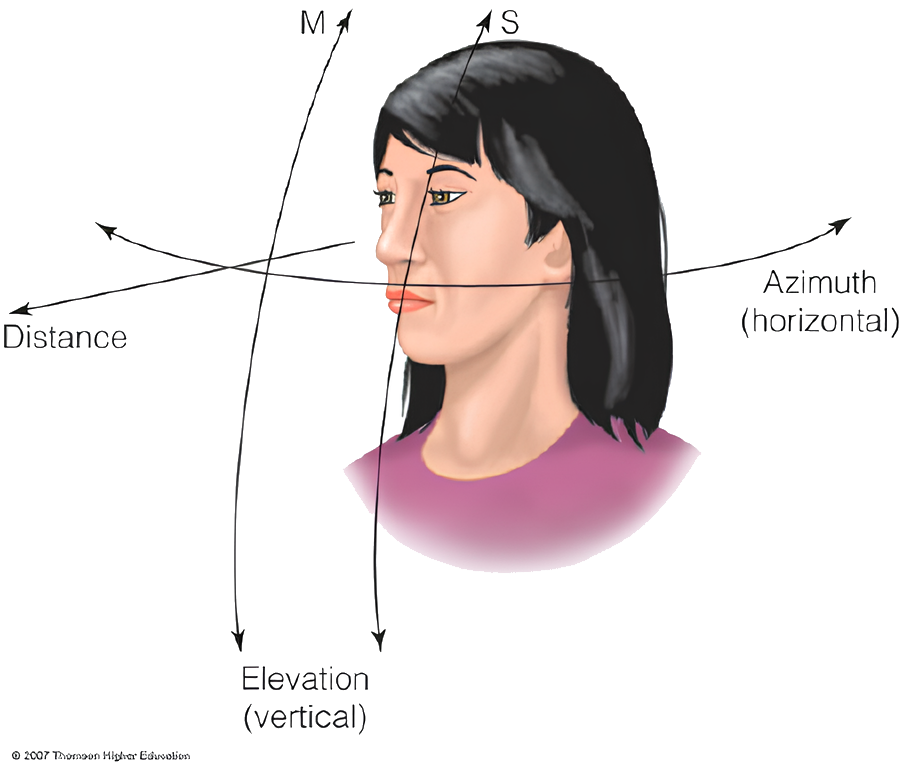
\includegraphics[width=0.5\linewidth]{Images/azim.png}
    \caption{How a sound source location is expressed: azimuthal angle, elevation angle and distance}
    \label{fig:intro-azim}
\end{figure}

\parspace

This task is essential and complex under multiple perspectives, which we will briefly outline here. Sound localization is fundamental for survival, whether predator or prey; it is a foundational part of extracting relevant sounds from a noisy environment; as such, it is common to many different species. And yet, although its usefulness is undeniable and we never question our ability to localize sounds, detecting and localizing air-borne sounds needs specialized physiological structures. When transmitted inside the ear, airwaves become fluid waves, which have a much higher acoustic impedance (i.e., how hard it is for sound to propagate); the structures to accomplish this and other needs\footnote{We will explore these throughout the text. Among them are comparing arrival times with sub-millisecond differences, analyzing a sound by frequency, and keeping up with sound features using neurons with very high firing rates.} developed several times independently in frogs, mammals, reptiles and birds (both sauropsids) \cite{clackEvolutionTetrapodEars1997}. This means findings obtained in different lineages (birds) may not exist in the mammalian brainstem. As we'll see later, this has been a significant complication of sound localization research. 

\parspace
Sound localization also features particular brain circuitry, which has properties not found in other areas of the brain. The need to extract auditory cues (\textit{active encoding}) is another unique feature of sound localization: for sight and somatosensation, the source of a stimulus is always at least partially present in how the sensory organ detected the stimulus in the first place; instead, the tympanic membrane does not explicitly express differences in source position.

Another complication of sound localization research, which has no doubt been one of the driving factors behind its long history, is that the nuclei responsible for this task are situated inside the brainstem, with small, difficult-to-detect potentials, in a location that's difficult to keep in a single brain slice together with its inputs or reach \textit{in-vivo}. 

\parspace
Summarizing, sound localization: 
\begin{inlinelist}
    \item is restricted to specific sensory inputs
    \item is involved in both main functions of auditory capability (the \textit{where} and the \textit{what})
    \item is implemented by specialized structures
    \item needs active encoding
    \item is solved by nuclei that are limited in number but difficult to reach and study
    \item has practical implications for a growing epidemic of hearing loss
\end{inlinelist}.
Due to these factors, sound localization is being actively researched for both academia and industry applications (ranging from healthcare to audio products to videogames\footnote{HRTF, defined later in the text, have been used for spatial audio in many videogames.}). In addition, these features also make it a perfect subject for study using computational methods: its limited focus in terms of input and number of involved neurons (compared to other brain areas) mean that neuronal simulations can be run as a whole; these simulations can be tweaked to experiment with specialized structures, features and theories; the dual interest from industry and research results in many of the components having existing models which strike a good balance between faithfulness and efficiency\footnote{Some of the peripheral auditory pathway needs to be run real-time on limited hardware, such as cochlear implants}. In addition, the need for some type of active encoding \textit{justifies} the use of computational models to enable researchers to understand the mechanism behind this encoding. Finally, testing a theory in a simulation before biological experiments limits animal research to a subset of biologically plausible hypotheses.


\subsection{Auditory Cues}\label{sec:cues}
To derive sound source position, the brain must decode how different positions affect the stimuli received by the two ears. These effects (\textit{cues}) can be classified as binaural and monaural. There are two types of binaural cues: the Interaural Time Difference (ITD) and the Interaural Level Difference (ILD). Monaural (or spectral) cues, instead, are all those experienced by a single ear as a sound moves through space. In this section, we will detail binaural cues by explaining how to calculate them, how they bias evolutionary adaptations, how the brain uses them, and how they can be modeled.

\begin{figure}
    \centering
    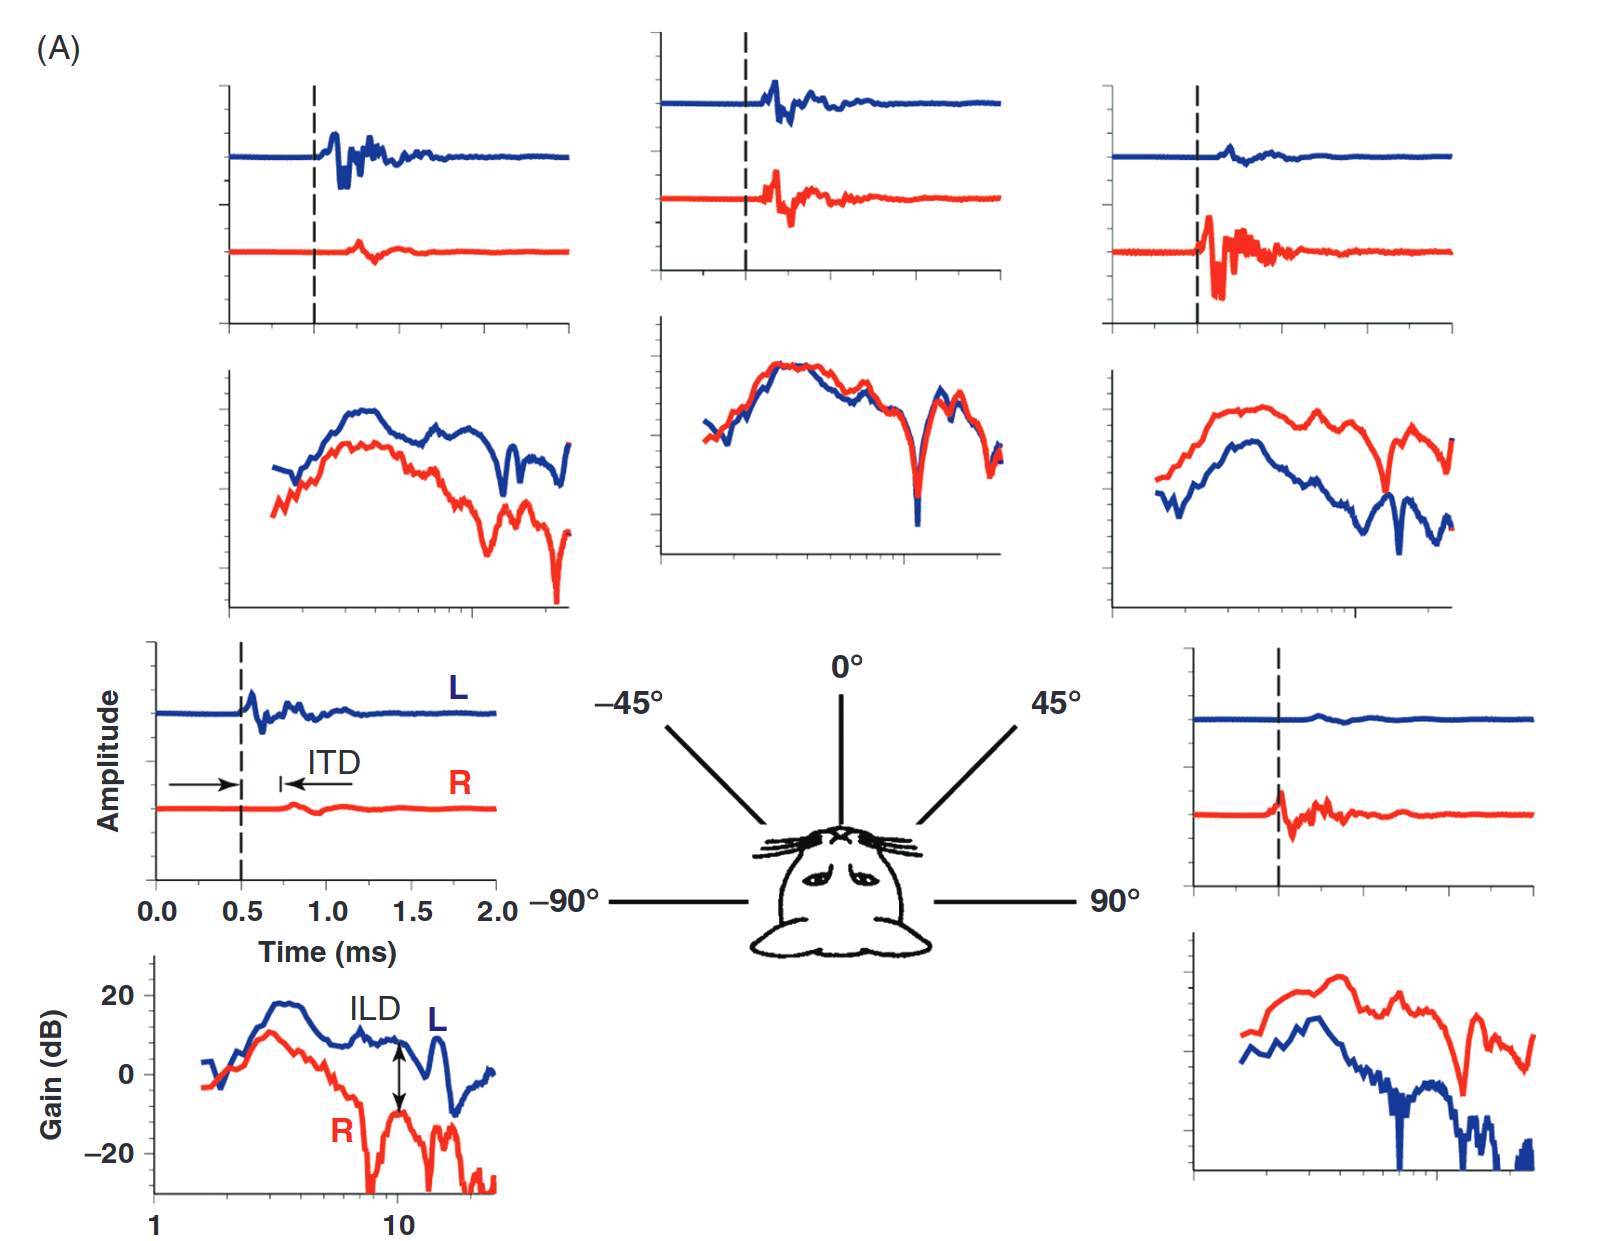
\includegraphics[width=0.45\linewidth]{Images/hrtf-cat-azim.png}
    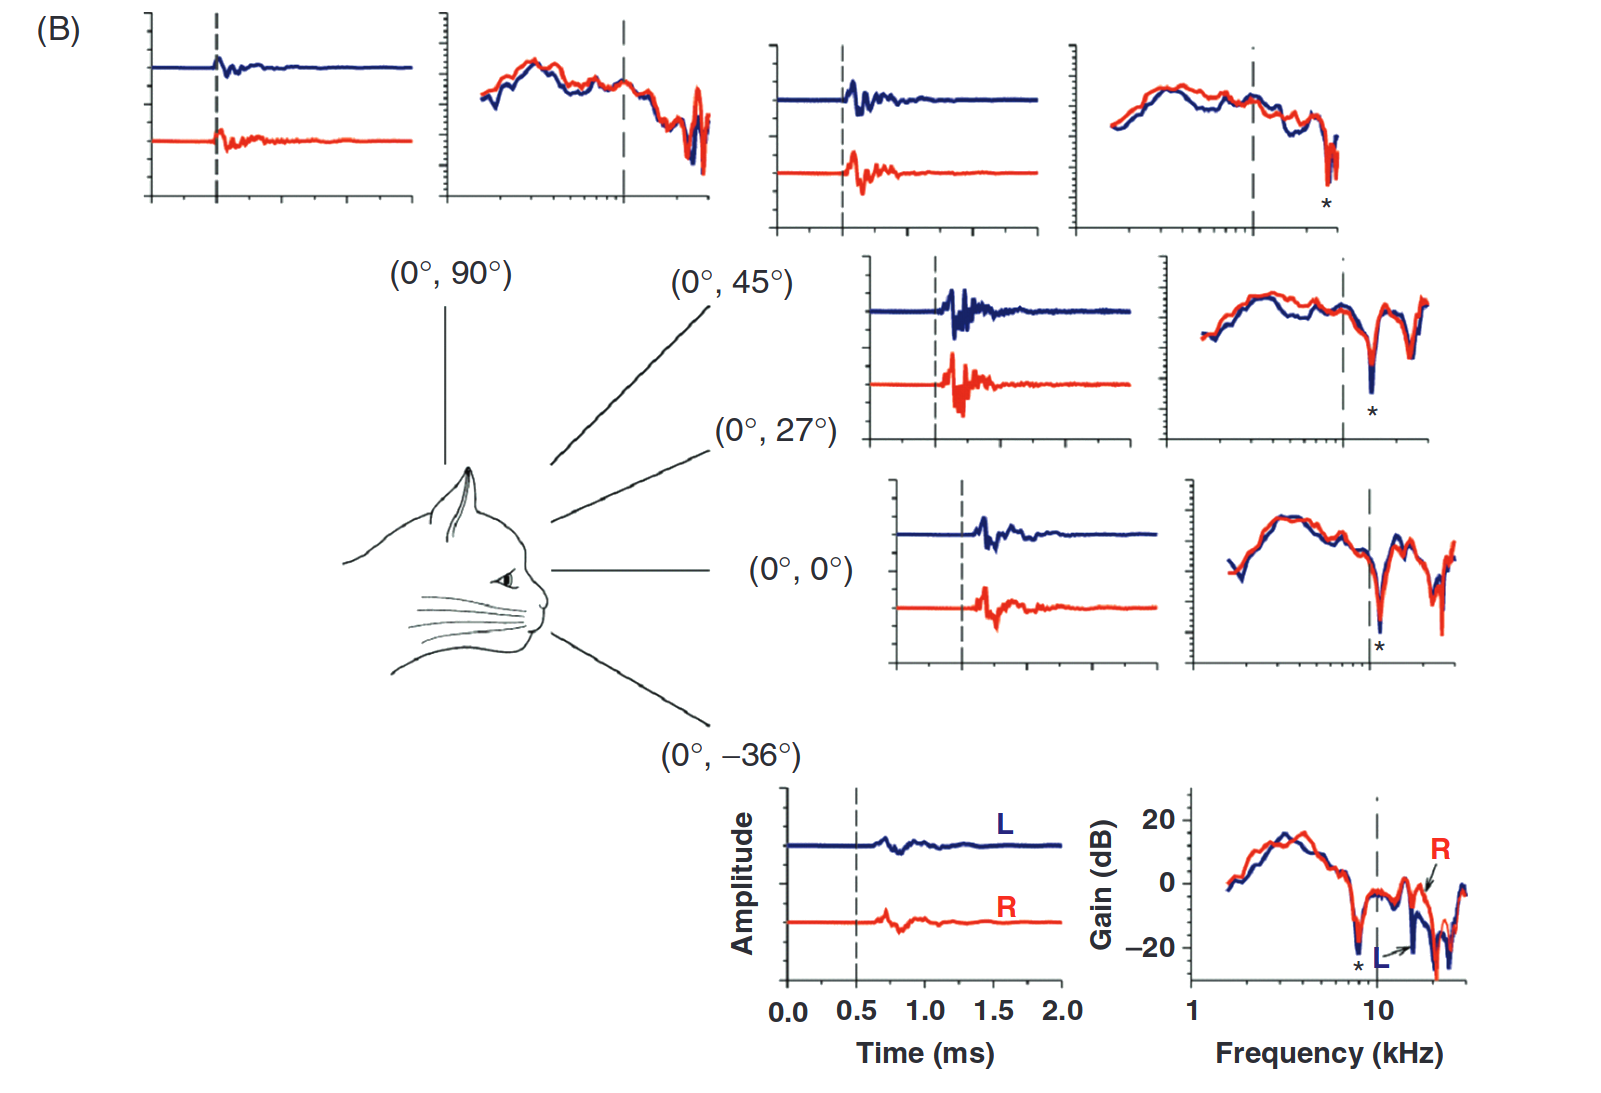
\includegraphics[width=0.44\linewidth]{Images/hrtf-elev.png}
    
    \caption{Effect of different azimuthal (A) and elevation (B) angles on sound and its spectrum. The impulse response for how a listener's environment and body composition affect sound arrival times, level, and spectral content is called the Head Related Transfer Function (HRTF). ITD and ILD are visible in (A), while (B) shows the spectral notch (see \protect\hyperlink{text:spectral-notch}{later}). From \cite{yinNeuralMechanismsBinaural2019}
    \label{fig:intro-hrtf}}
\end{figure}


\parspace
To understand auditory cues, there are two fundamental properties of auditory processing biology that we will mention (detailed explanation in sections \ref{bio-IHC} and \ref{bio-BM}) before all else: phase locking and tonotopical organization. The first refers to the property of Auditory Nerve Fibers (ANFs) to fire at a specific phase of a sound, hence maintaining information about its frequency and relative arrival phases\footnote{If both pathways are of the same length, then the relative arrival time (or arrival phase) is discernable by comparing the two phase-locked responses. More detail in \ref{bio-binaural}}; this association is maintained until a threshold of 3 to \qty{5}{\kilo\hertz} \cite{yinNeuralMechanismsBinaural2019}. Tonotopical organization, instead, means that all nuclei involved are organized by frequency; intuitively, higher-level nuclei receive an approximate spectrum of the sound.
The two binaural cues we mentioned are part of the ``duplex theory'', first formalized by Lord Rayleigh \cite{rayleighXIIOurPerception1907}, according to which localizing sounds on the azimuthal direction is based on these cues. The first cue is the Interaural Time Difference (ITD): the difference in time that the sound wave takes to get to one ear compared to the other\footnote{Tonotopical organization allows this comparison to happen, as it allows to compare specific frequencies}. Although simple to understand, it requires special care by the brain, as its full range is only around \qty{1.3}{\milli\second} (considering an ideal head of width \qty{22}{\centi\meter}); meanwhile, the average duration for a spike event in a neuron is closer to \qty{1}{\milli\second}\footnote{This means that there must be some mechanism to move from the realm of minute differences in timing ($\simeq\qty{10}{\micro\second}$) to differences in spike events per second.}. 

The second binaural cue is the Interaural Level Difference: this represents the shadowing effect that the head has on the level (loudness) of sounds arriving at each ear. The magnitude of this shadowing depends on the ratio between head size and wavelength/frequency: when the wavelength is smaller than the head size, significant shadowing occurs; in general, higher frequencies are shadowed more and lower frequencies are shadowed less \ref{fig:intro-hrtf}. Hence, all animal sizes can experience significant ILDs, but the threshold frequency at which these become significant varies depending on head size. This does not mean there is a fixed threshold at which only one of these cues is valid, but their respective effectiveness for each head size rises and falls depending on the frequency.

\parspace

These binaural cues are not enough to account for all positions in space, but only in the azimuthal dimension: for each pair of ITD and ILD, a cone of possible locations exists that satisfy the ITD and ILD values. In addition, other pieces of psychoacoustic evidence are unexplained by binaural cues, e.g., how sounds heard from speakers are perceived as ``external''. In contrast, from earphones, they are perceived as ``internal''. These \textit{missing pieces} are broadly referred to as monaural cues: they account for how the outer ear affects the sound depending on its location. The most common example of the \hypertarget{text:spectral-notch}{spectral notch}: the shape of the pinna introduces a masking effect on a narrow set of frequencies; the frequencies depend on the sound source location, specifically the vertical angle.

\parspace

The compound effect of delays, attenuations, cancellations, and amplification of a sound traveling from its source to the two ears is called the Head Related Transfer Function (HRTF). Although only the head is mentioned, they account for all the transformations a sound goes through when going from the source to the two ears; as such, HRTFs have three inputs (a source sound, with its azimuth and elevation angles) and two outputs (the sounds as perceived inside the ear canals); depending on the dataset, an HRTF may also need the distance from the listener, while other datasets do not allow for varying distances. Specifically, when distances are above \qty{1}{\meter} (far-field region), distance can be accounted for by scaling sound level according to the inverse square law, as HRTFs are asymptotically distance-independent \cite{brungartAuditoryLocalizationNearby1999}. In contrast, in the near-field proximal region, HRTFs are affected by distance. \label{extra:hrtf_diff} Measuring an individual's HRTF is time-consuming\footnote{Although recently, new methods have risen to tailor HRTFs to individuals in home environments \cite{wolfImplementingContinuousAzimuthBinaural2020}, more in \cite{wolfImplementingContinuousAzimuthBinaural2020}
}: it requires multiple measurements, either with in-ear microphones and a speaker or with in-ear speakers and a microphone, with the subject in an anechoic chamber; careful tuning and postprocessing are required to pick a physiologically safe sound level, increase signal-to-noise ratio, suppress background noise and unwanted reflections in measurement results. Once the measurements are complete and fully processed, obtaining the transfer function is easily achieved by moving to the frequency domain. Some generalized HRTF models are available, although they may reduce localization accuracy \cite{wolfImplementingContinuousAzimuthBinaural2020}.


The interest in HRTF is not driven only by research purposes but also by industry application: filtering sounds with HRTFs is an efficient way to create virtual acoustic environments (VAEs), which has found its uses in virtual, augmented and mixed reality, but also videogames\footnote{In Valorant, Riot Games even calls its setting ``HRTF'' \cite{WhatValorantsHRTF2021}}.

\subsubsection{Evolutionary perspective and consequences}

The relationship between head size and acoustic cue effectiveness has an evolutionary background worth reviewing. To detect and localize air-borne sounds, an animal needs specialized structures (the middle ear) to amplify air pressure waves, and these structures evolved independently in different lineages: mammals, frogs, and sauropsids (reptiles and birds). Fossil studies show that this parallel evolution developed structures (absent in their ancestors) around the triassic \cite{allinEvolutionMammalianMiddle1975}. Although this likely means they were under a common evolutionary pressure, it does not mean their solutions for this pressure were the same, as their pre-existing conditions (anatomy and lifestyle) differed: 
\begin{itemize}
    \item Sauropsids were larger, both in overall body size and head size. This meant larger ITD differences, which entails less of a need for highly specialized neuronal processing. It also means a preference for lower frequencies, which makes higher frequencies, where significant ILDs are more likely to occur, less relevant.
    \item Early sauropsid middle ear (and current frogs) only uses a single middle-ear bone, favoring low-frequency sound conduction. Instead, the mammalian middle ear has always been a three-boned structure favoring higher-frequency conduction \cite{manleyEvolutionaryPerspectiveMiddle2010}.
\end{itemize}
Most likely, the sound localization system in birds (inherited from dinosaurs) evolved to process ITDs to handle low-frequency sounds. Instead, in mammals, where
\begin{inlinelist}
    \item the inner ear does not conduct low frequencies efficiently;
    \item ancestors' heads were smaller sizes, which made it much more difficult to detect ITDs;
    \item most small mammals today rely on ILDs;
\end{inlinelist}
mammalian ears likely developed to handle high-frequency sounds, using ILDs, and only later included ITD processing \cite{grotheNaturalHistorySound2014}.

\parspace

This evolutionary perspective has two consequences: 
\begin{description}
    \item \textbf{Different lineages may have different strategies.} There is evidence \cite{carrCircuitDetectionInteraural1990} for a mechanism to detect ITDs in the nucleus laminaris of the barn own. Broadly, using delay lines (i.e., longer and slower axons), internal delays are created, which compensate the external ITD; then, the targets can act as coincidence detectors (a known feature of neurons), where only the one with the correct (i.e., corresponding) delay fires, hence identifying the current ITD. This type of processing, the corresponding map of internal delays, and its related properties were not found in mammals \cite{yinNeuralMechanismsBinaural2019}. Still, mammals recognize ITDs, so they must use a different strategy to perform the same function.
    \item \textbf{Different nuclei are dedicated to different auditory cues.} As we will see in the next section, ILDs and ITDs are primarily processed in different nuclei with a shared pathway. Specifically, the structure processing ILDs, where binaural inputs first meet, is the lateral superior olive (LSO), and it is homogenous in all mammals investigated \cite{tollinLateralSuperiorOlive2003}.
\end{description}

\subsection{Input types and behavioral results}\label{sec:intro-input}
In this brief section, we introduce sound types, which we will reference throughout the text, and recap some of the behavioral results that will inform the evaluation of our results.
For our concerns, sounds can be classified by frequency and level. Humans can hear sounds ranging from \qty{20}{Hz} to \qty{20}{\kilo\hertz}, with higher frequency hearing degrading most with age. Safe levels for humans are up to 90-\qty{100}{\deci\bel}. Pure tones are sounds with a sinusoidal waveform, so they have constant frequency, phase shift, and amplitude. Because of these features, tonnes will be featured most prominently in our work since they allow us to selectively investigate a specific frequency due to the tonotopical nature of sound processing. The two other sound types featured in this work are white noise and clicks. White noise is a random signal with equal power at all frequencies, making it perfect for masking other signals. Lastly, clicks are brief, broadband (thus stimulating the entire frequency spectrum) stimuli, sometimes called transients, which can be used to study timing.

In behavioral studies, humans show higher accuracy in the localization of broadband signals than pure tones and cannot achieve vertical localization without spectral cues. As expected from section \ref{sec:cues}, front-back confusions are common \cite{hillResolutionFrontbackConfusion2000} and sometimes counted as correct in early results. It is unclear whether accuracy improves with louder sounds (within safe thresholds) or longer expositions \cite{yostSoundSourceLocalization2016}. The sound localization ability is also studied regarding its sensitivity, i.e., the just noticeable difference (JND), usually expressed as the minimum audible angle (MAA), from a reference sound. In a critical result by Mills, the MAA was measured as a function of the azimuthal position of the reference sound: the MAA systematically grew as the reference sound moved away from zero degrees (in front of the subject).


\subsection{Sound Processing}\label{sec:model-periph}
This section will review the auditory pathway and how to model it. It will be organized in parallel, pointing out relevant anatomical features and explaining how they can be modelled. Because our focus will be on the features relevant to sound localization, much will be omitted. At a high level, the auditory pathway begins outside the body, as the environment and the outer ear modify sound, which causes the eardrum to vibrate. This vibration is analyzed, modified, and transmitted as a graded potential, which becomes the input for the first neural component. Further neural connections then enhance the signal and transmit it to the processing nuclei in the brainstem.
We split the pathway into three sections: first, the peripheral system, which is composed of all sound processing structures that are not neural in nature; then, the monaural neural pathways, which filter and convey sound signals to the processing nuclei; finally, the binaural section, where inputs from the two ears first meet, which perform part of the comparisons and terminate in the brainstem.

\subsubsection{Peripheral System}
The sequence of transformations starts outside the body, as sound is affected by the head, torso, and outer ear until pressure waves cause the eardrum to vibrate. Small ossicles in the middle ear amplify and transmit the eardrum vibration to the cochlea. The vibration becomes fluid waves in the cochlear fluid, which causes the basilar membrane (BM) inside the cochlea to respond; the movement of the BM is further modified by outer hair cells (OHCs) and detected by inner hair cells (IHCs), which transduce the motion into fluctuations of a graded potential which controls neurotransmitter release. These neurotransmitters activate the first neural step, the auditory nerve fibers (ANFs).

In the following paragraphs, a commonality of all modeling work arises: modelers must strike a balance between white-box, bioplausible (mechanical or otherwise), computationally expensive simulations and grey-box system identification to obtain computationally less expensive, more opaque models.

\paragraph{Outside and Outer ear}
We have already mentioned how traveling from sound source to the two ears changes the sound: due to diffractions, scattering, interference and resonance, by the body and obstacles, attenuation, cancellation and amplification can be observed, and the spectral content of the signal changes. Two possible routes have been explored to reproduce HRTFs: simulating a physical model or creating a digital filter. By simulating a physical model of the sound waves interacting with anatomical features and the room \cite{walshBoundaryElementModeling2004}, it is possible to not only understand how each feature affects the result but also to adapt it to different subjects or environments; these methods are very computationally expensive. On the other side, it is possible to create a digital filter that reproduces the sampled experimental data \cite{kulkarniInfiniteimpulseresponseModelsHeadrelated2004}, where the complexity is always lower and can be further lowered with simpler filters (provided they capture sufficient features of the HRTF). Although vastly more efficient, these digital filters do not provide any insight into the effect of individual anatomical components.

\paragraph{Middle Ear}
As the eardrum vibrates, three ossicles, the malleus, the incus, and the stapes, transmit the vibration to the oval window. A combination of the low surface area ratio between the eardrum and stapes footplate and the lever ratio of the ossicles allows the middle ear to move the low-impedance (air vs. fluid), low-pressure, large-displacement vibrations into higher-impedance, higher-pressure, small-displacement vibrations in the cochlear fluid\footnote{Otherwise, sound airwaves would just bounce away: try screaming at a friend underwater.}. The middle ear does not introduce distortions at physiologically safe levels, but the filtering effect is not linear \cite{ruggeroMiddleearTransmissionHumans2003}. Modeling approaches follow under three categories: lumped-element models \cite{rosowskiModelsExternalMiddleEar1996}, biomechanical models \cite{ganThreedimensionalModelingMiddle2002}, and digital filters \cite{tanPhenomenologicalModelResponses2003}\cite{holmesTemporalRepresentationSpeech2004}. The first use the parallel between acoustic and electrical elements, and consider the middle ear a transmission line with lumped electrical models of elements; this was the classical modeling technique, and it is now less common. Biomechanical models reconstruct the geometry of the elements in a physics simulation and (as in the outer ear) are computationally expensive but allow for fine-grained investigation of healthy or impaired tissues on sound transmission. The third class of models, digital filters, use either filter cascades or a single filter to achieve realistic frequency responses, multiplied by a scalar for a realistic gain \cite{meddisAuditoryPeripheryPinna2010}. Some authors \cite{cheathamInnerHairCell2001}\cite{tanPhenomenologicalModelResponses2003} suggest that the middle ear is responsible for the asymmetries in basilar membrane responses (both for iso-intensity curves and so-called glide or chirp, more on this later).


\paragraph{Basilar Membrane and Outer Hair Cells}\label{bio-BM}
As the stapes vibrates on the oval window, its vibrations are transmitted to the cochlear fluid, creating a pressure wave. This fluid is contained in two connected chambers (through the helicotrema) at the apex, the scala vestibuli and the scala tympani. The endings of this two-chamber system are both sealed but flexible: on the side of the stapes, the oval window can flex (to transmit stapes vibrations), while on the opposite side, the round window is flexible as well. This allows the pressure wave to be created. As the fluid (incompressible), moved by the wave, pushes and pulls on the bottom of the chamber (basilar membrane), the basilar membrane moves up and down, creating what's called the ``traveling wave''. Because of varying width and stiffness, different points of the BM respond to different frequencies: the base of the BM responds to high frequencies, while the apex vibrates at low frequencies, with frequencies arranged logarithmically \cite{javelAuditorySystemPeripheral2003}. Thanks to this, the inner ear can organize sounds by frequency (performing an approximate spectrum); this distribution is called tonotopic organization.\footnote{The traveling wave starts at the base of the BM, increasing in amplitude until it gets to the frequency of the input sound}. The BM is also the base of hair cells, and each placement of hair cells is usually called ``site''. There are two types of hair cells: inner hair cells (IHCs) and outer hair cells (OHCs). The first (IHCs) are responsible for transducing mechanical signals into electrical; the second (OHCs) are the active component of the cochlea \cite{hopkinsChapter27Deafness2015}, as they modulate basilar membrane motion, both increasing sensitivity and enabling frequency selectivity in complex sound environments \cite{ruggeroFurosemideAltersOrgan1991}. We will consider this active effect part of the BM modeling, as this is the most common approach. 

Each BM site responds to a small range of frequencies, centered around the frequency of maximal response, called \textit{characteristic frequency}(CF), with responses tapering off at nearby frequencies. Due to this, every BM site is modeled as a frequency filter, with the whole BM being a series (\textit{bank}) of overlapping filters. These filters are asymmetric in two dimensions: 
\begin{inlinelist}
    \item the response strength of a single site increases slowly for frequencies below the CF but tapers off quickly above it;
    \item the instantaneous CF of a single site changes during a brief stimulus (like a click), increasing at the basal site and possibly decreasing at the peak (\cite{carneyFrequencyGlidesImpulse1999} vs \cite{lopez-povedaPsychophysicalEstimatesLeveldependent2007}), a phenomenon called chirp or glide.
\end{inlinelist}
There are various nonlinearities in BM filter response \cite{lopez-povedaSpectralProcessingPeripheral2005}: they show more gain at low levels than high (growing compressively with level); both CF and bandwidth (how wide the set of nearby frequencies the site responds to) change depending on level; two-tone suppression (the response to one tone decreases when paired with a different tone); distortion. These responses depend on the physiological state of the cochlea: as they depend on active components (OHCs) \cite{hopkinsChapter27Deafness2015}, they become fully linear post-mortem. 

BM model classes are the same as previous components (transmission line, biomechanical, digital filters). Given the breadth of approaches, we will focus on the ones relevant to our investigation: digital filters. The most common classical model is the gammatone filter \ref{fig:coc-gammatone-vs-gammachirp}, developed to simulate auditory nerve fiber responses. The response of the gammatone filter is the product of a tone (at frequency equal to the CF of the BM site) and a gamma distribution that determines how adjacent frequencies are also involved. To model the entire BM, it is approximated to a series of gammatone filters with increasing CF, a filter bank. This filter is linear, and symmetric in its response. Improvements to the original gammatone led to the gammachirp filter, which was not symmetric in its response, by modulating the aforementioned tone in frequency: from here, the chirp name. After further improvements, the filter became the compressive gammachirp \cite{irinoCompressiveGammachirpAuditory2001}, composed of three simple filters: first, the gammatone filter followed by a low-pass filter, which combined produce the asymmetric gammatone-like filter; then, a high-pass filter modulated by frequency, which accomplishes the level-dependent gain (compression).


The compressive gammachirp accurately reproduces human auditory filters over many center frequencies and levels, and \enquote{could probably be used to simulate physiological BM iso-intensity responses directly, although no studies have been reported to date aimed at testing the filter in this regard} \cite{meddisAuditoryPeripheryPinna2010}. Although the frequency glide is included, the trends (the direction of the shift compared to level) are inconsistent with physiological data. It is likely unable \cite{plackLinearNonlinearProcesses2002} to reproduce two-tone suppression and more advanced combination effects. More advanced models exist: the Tan-Carney model \cite{tanPhenomenologicalModelResponses2003}, a gammatone filter where gain and bandwidth vary dynamically to account for the nonlinear properties; the Dual Resonance NonLinear (DRNL) \cite{lopez-povedaHumanNonlinearCochlear2001}, composed of the sum of a linear and a nonlinear pathway, which can also be adjusted to simulate OHC loss (more detail later). Because of our narrow focus on sound localization, and since our investigation will primarily focus on single tones, the most complex and faithful models are outside the scope of this work: the features they reproduce are not shown in higher localization neural nuclei, and their computation time is much higher than simple models.

\paragraph{Inner Hair Cells}\label{bio-IHC}
As the cochlear fluid and the BM of a single site vibrate, the hair cells in the organ of Corti are moved back and forth. Specifically, the inner hair cells (IHCs) are responsible for the transduction of mechanical to electrical signal. IHC stereocilia are organized in bundles, with their tips connected by links: when deflected towards the tallest of the bundle, the links pull open ion channels (potassium) to increase the inward flow of ions that depolarize the cell; when deflected in the opposite directions, ion channels are closed to prevent the flow of ions inside the cell. As the voltage inside the cell changes, voltage-gated calcium channels are opened and closed, and calcium ions promote the release of neurotransmitters (glutamate) into the synaptic cleft. This \textit{graded potential} is then picked up by the auditory nerve fibers (ANFs). This means the signal is only transduced in one direction (asymmetric gating of the ion channels), which gives the IHCs the characteristic feature of half-wave rectifiers. This also means that the concentration of ions will be at maximum at the moment corresponding to a specific sound phase, which causes the following neurons to be \textit{phase locked}. This results in a complex environment where the intracellular voltage is determined by
\begin{inlinelist}
    \item inward potassium flow, driven by stereocilia movement
    \item outward potassium flow, to compensate the inward, at the basolateral membrane
    \item inward calcium ions, that cause the neurotransmitter release
    \item a capacitive effect of the IHC membrane (which results in a low-pass filter)\footnote{Consider a simple half-wave rectifier with a capacitance: as the frequency rises, between cycles the capacitance will have to provide current for less and less time. Hence, high frequencies will be masked, while low frequencies, in which the capacitance has time to deplete, will be reflected in the output.}
    \item the homeostasis of the organ of Corti.
\end{inlinelist}
In addition, it is difficult to isolate the contribution of the IHC from those of the middle ear and the BM; this contribution is estimated by measuring the growth of the AC and DC components while changing the level of an input sound at a frequency \textbf{below} the CF so that the BM effect is almost linear (the middle ear, as we said, stays linear). The result also reflects the effect of the IHC membrane (and likely other factors \cite{weissComparisonSynchronizationFilters1988}), which limits the AC effect (phase locking) to frequencies below \qtyrange[range-units=single,range-phrase=\,to\,]{3}{5}{\kilo\hertz}; below this threshold, the AC component matches the stimulus frequency, while the DC component matches the stimulus level.
As can be imagined from our description, a biophysical approach is to model the IHC with an electrical circuit: this results in accurate response characteristics across different datasets \cite{lopez-povedaBiophysicalModelInner2006}. Alternatively, digital filter approaches use a series of asymmetric gains (up to a saturation point), followed by a low-pass filter for the capacitive effect of the membrane. Their shortcomings are as earlier: they do not allow for physiological inspection, cannot model non-healthy IHCs, and are less accurate than biophysical models.
\begin{figure}
    \centering
    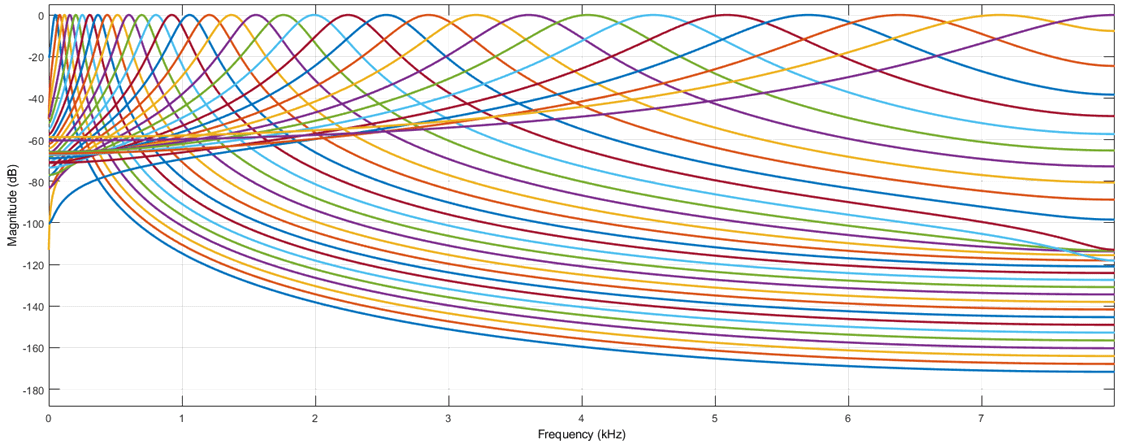
\includegraphics[width=0.8\linewidth]{Images/gammatone.png}
    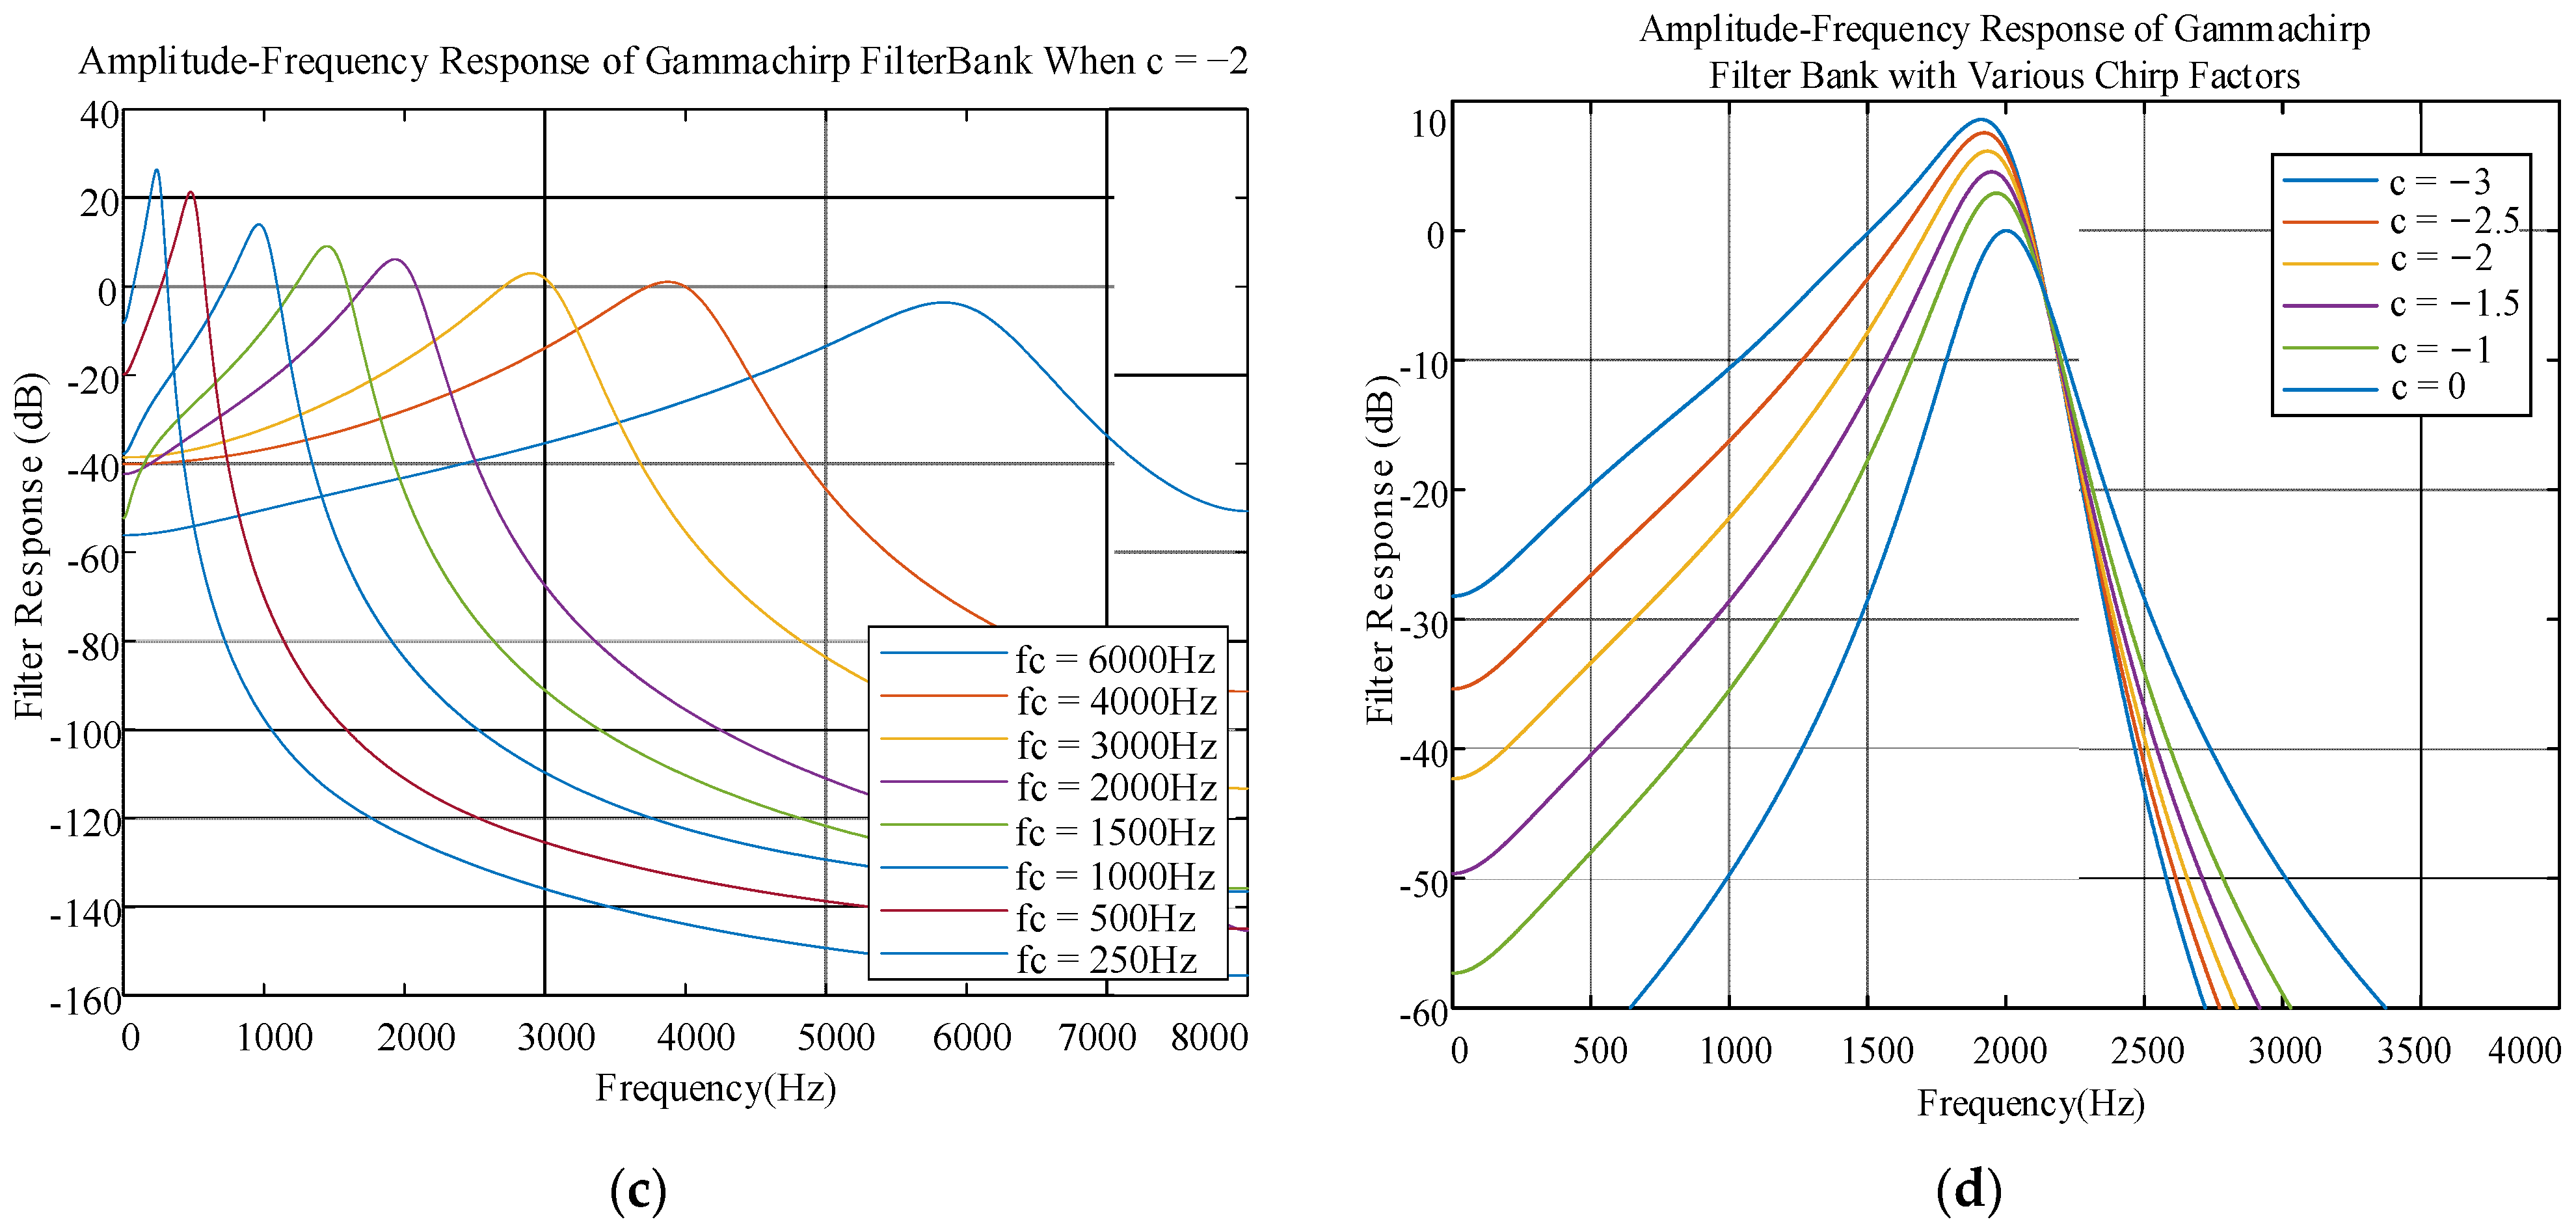
\includegraphics[width=0.8\linewidth]{Images/gammachirp-bank.png}
    \caption{Differences between gammatone (top) and gammachirp (bottom) amplitude/frequency responses. As the characteristic (central) frequency increases, the bandwidth of the filters increases. CFs are spaced exponentially, but in gammatone filters the frequency response of each filter is symmetric about the CF. Gammatone filters also do not modulate peak response. From MATLAB documentation \cite{GammatoneFilterBankGammatoneFilter} and \cite{guoDesignMethodGammachirp2022}.}
    \label{fig:coc-gammatone-vs-gammachirp}
\end{figure}


\paragraph{Auditory Nerve Synapse}
The connection to the auditory nerve is achieved by releasing glutamate (the neurotransmitter) into the synaptic cleft. This depends both on the voltage of the IHC and the availability of vesicles in the presynaptic area. During an extended stimulus, lower availability will cause lower activation, which causes the AN spike rate to fall. This phenomenon is called ``adaptation''. Hypothesizing a single reservoir of vesicles would entail a single time constant of adaptation; instead, due to data indicating multiple constants, two similar models have been proposed: the first based on multiple successive reservoirs \cite{carneyModelResponsesLowfrequency1993}, the second on reuptake from the synaptic cleft \cite{meddisAuditorynerveFirstspikeLatency2006}, and as reviewed by one of the authors the models are mathematically similar \cite{zhangAnalysisModelsSynapse2005}. The exact connection between vesicle release and AN spike is unknown \cite{meddisAuditoryPeripheryPinna2010}, so it is usually modeled probabilistically. In our case, this probability will be collapsed in a realization, as we need real spikes for the remainder of the network.
\parspace

\begin{figure}[H]
\centering
    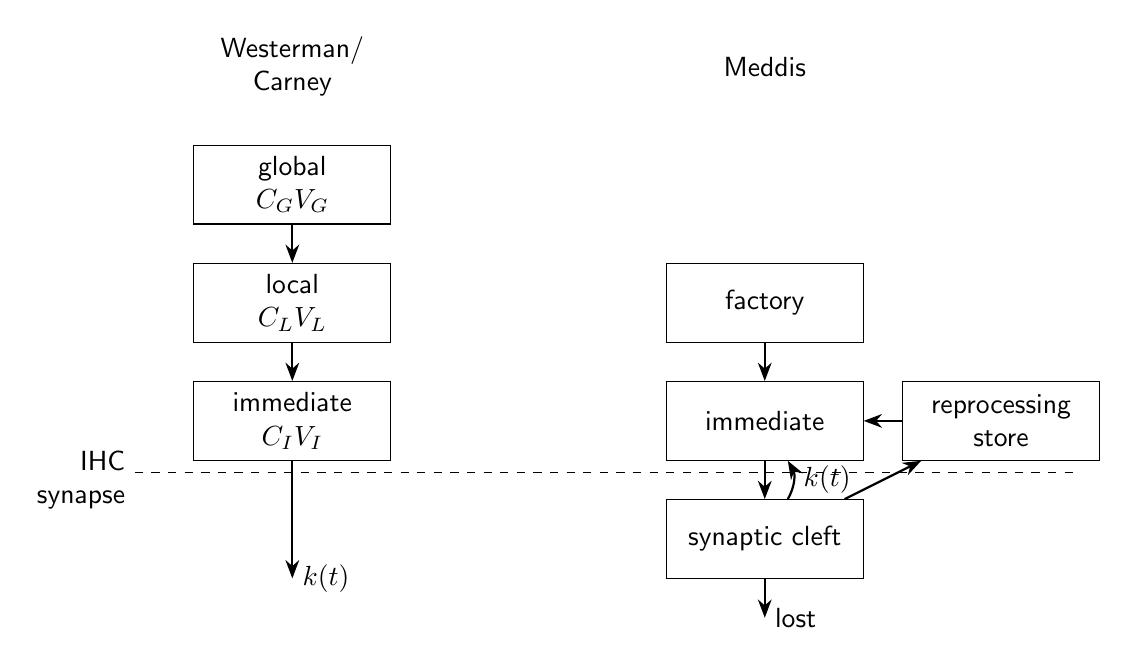
\begin{tikzpicture}[
        node distance = 1.5cm,
        box/.style = {draw, minimum width=2.5cm, minimum height=1cm},
        arrow/.style = {-Stealth, thick},
        every node/.style = {font=\sffamily}
    ]
    
    \node[align=center] at (0,4.5) {Westerman/\\Carney};
    \node[align=center] at (6,4.5) {Meddis};
    
    \node[box,align=center] (global) at (0,3) {global\\$C_G V_G$};
    \node[box,align=center] (local) at (0,1.5) {local\\$C_L V_L$};
    \node[box,align=center] (immediate) at (0,0) {immediate\\$C_I V_I$};
    
    \node[box] (factory) at (6,1.5) {factory};
    \node[box] (immediate2) at (6,0) {immediate};
    \node[box] (synaptic) at (6,-1.5) {synaptic cleft};
    \node[box,align=center] (reprocessing) at (9,0) {reprocessing\\store};
    
    % Arrows
    \draw[arrow] (global) -- (local);
    \draw[arrow] (local) -- (immediate);
    \draw[arrow] (immediate) -- (0,-2) node[right] {$k(t)$};
    \draw[arrow] (factory) -- (immediate2);
    \draw[arrow] (immediate2) -- (synaptic);
    \draw[arrow] (synaptic) -- (6,-2.5) node[right] {lost};
    \draw[arrow] (synaptic) to[bend right] node[right] {$k(t)$} (immediate2);
    \draw[arrow] (synaptic) -- (reprocessing);
    \draw[arrow] (reprocessing) -- (immediate2);
    
    % Horizontal line for IHC/synapse division
    \draw[dashed] (-2,-0.65) -- (10,-0.65);
    \node[left,align=right] at (-2,-0.75) {IHC\\synapse};
    
    \end{tikzpicture}
\caption{The Carney model for IHC-ANF synapse compared to the Meddis model. From \cite{meddisAuditoryPeripheryPinna2010}}
\end{figure}

\subsubsection{Monaural Neural Pathway}
Starting with the ANFs, the input becomes neural in nature. These inputs are filtered by bushy cells, then faithfully carried to both sides to be processed by higher centers in the superior olivary center (SOC). We will focus on the pathway generally associated with azimuthal localization, leaving aside the pathway handling spectral cues for the vertical direction. Monaural signals are then integrated by the lateral superior olive (LSO) and the medial superior olive (MSO), respectively associated with ILD and ITD.

\paragraph{Auditory Nerve Fibers}
So far, we've only considered afferent ANFs (from the cochlea to the central nervous system), but about 10\% of ANFs are efferent going from the brainstem back to the cochlea. The mechanism driving efferent fibers is still unclear and rarely included in models, so they are outside the scope of this work. Afferent fibers are classified in type I and type II, respectively 90\% (innervating IHCs) and 10\% of ANFs (for OHCs). Very little about type II fibers is known, but recent evidence suggests they may respond in case of OHC damage, carrying nociceptive information. Our focus will be on afferent, type I ANFs.


\begin{figure}
    \centering
    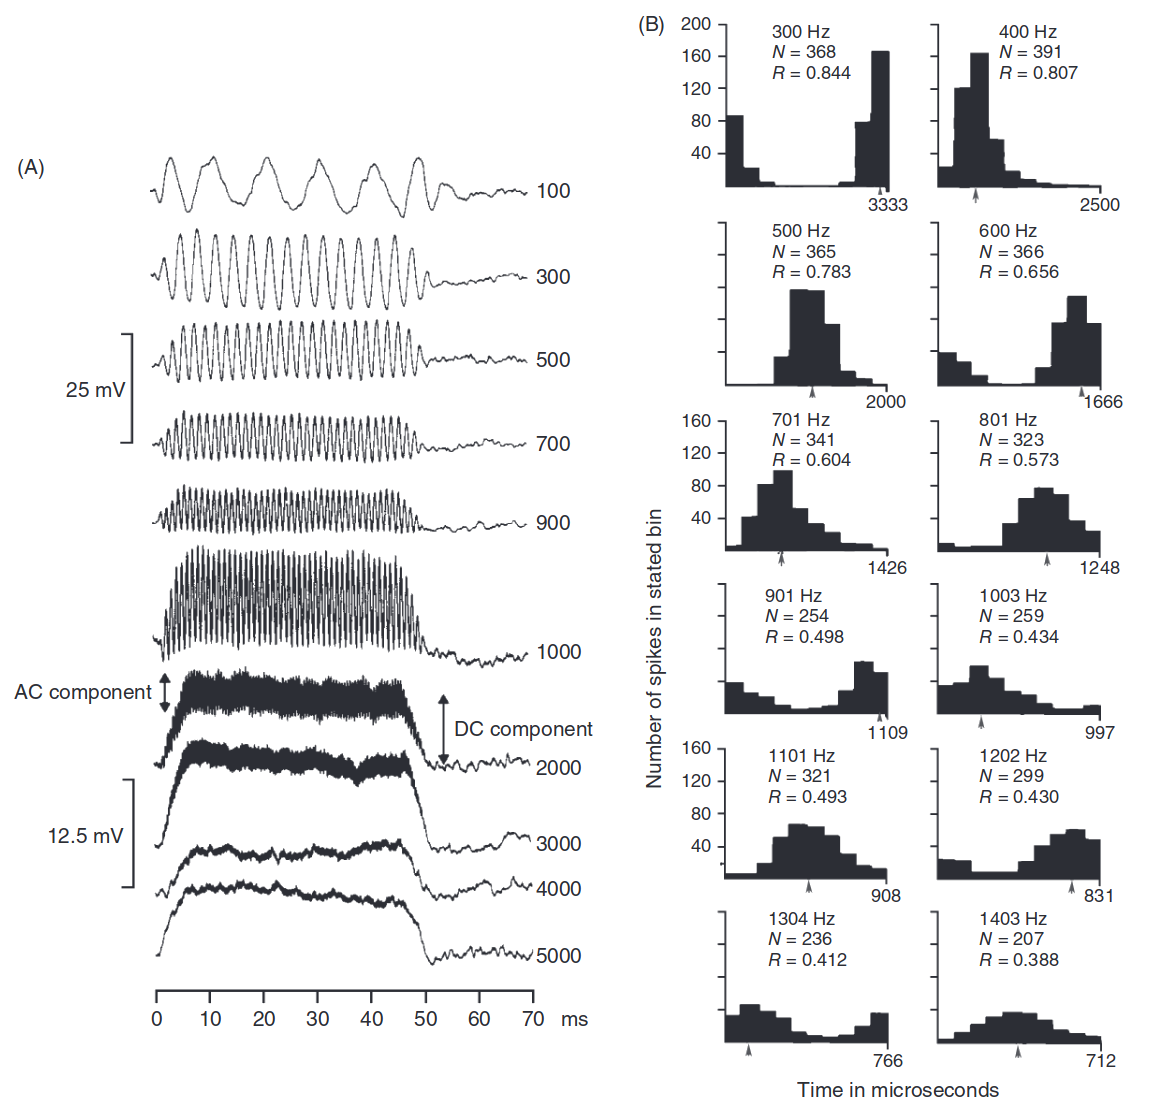
\includegraphics[width=0.6\linewidth]{Images/real_cochlea_phaselock.png}
    \caption{How phase locking and vector strength evolve with changing frequency/CF ratio in IHC (left) and ANF (right). In (A), the intracellular potential of an IHC from a guinea pig presented with tones at 80dB, varying in frequency. In (B), spikes from a squirrel monkey stimulated with tones organized in histograms show how much the ANF was phase-locked to a specific phase. Vector strength is noted in each. The CF of the fiber is 1100 Hz. From \cite{yinNeuralMechanismsBinaural2019}}
    \label{fig:real-ihc-anf-phaselock}
\end{figure}

Every IHC is innervated by ten to thirty type I ANFs, summing up to about 30,000 in total \cite{spoendlinAnalysisHumanAuditory1989}. ANFs innervate a single IHC, maintaining the IHC frequency tuning and showing phase-locking, and generate spontaneous spikerates (SR) of up to 100 spikes/s. All ANFs terminate in the cochlear nuclei (CN): after entering through the nerve root area, they bifurcate, with one branch going rostrally\footnote{In the general direction of the face} to the antero-ventral cochlear nucleus (AVCN) and the other caudally\footnote{In the general direction of the back of the head} to the postero-ventral cochlear nucleus (PVCN) and then the dorsal cochlear nucleus (DCN). The latter's functions are coding for spectral cues for vertical sound localization, filtering uninformative self-generated sounds, and processing of ultrasonic vocalizations \cite{yinNeuralMechanismsBinaural2019}. Although there are multiple cell types in the AVCN, the majority (and what we will focus on) are bushy cells, named after their bush-like dendritic tree. There are two types of bushy cells: globular bushy cells (GBCs) and spherical bushy cells (SBCs).

\paragraph{Bushy cells}
Due to a specialized set of currents, bushy cells have a very short membrane time constant, hence the quick decay of EPSPs. The fast decay entails that for bushy cells to spike they need either many coincident inputs or few very large inputs. Other cells, such as MSO, LSO, and cells in the MNTB, have since been discovered to have similar properties \cite{khuranaDynamicInteractionIh2011}\cite{yinNeuralMechanismsBinaural2019}. 
SBCs receive one to four of the largest ANF terminals (end bulbs of Held) on their soma, with large, often suprathreshold EPSPs generated. Due to this, their response is very similar to ANFs, a response called primary-like \cite{pfeifferClassificationResponsePatterns1966}; this also means that SBCs stay phase-locked at low frequencies, remarkably even more accurately than ANFs \cite{jorisEnhancementNeuralSynchronization1994}. Axons of SBCs then project directly to the ipsilateral LSO and both MSOs.
GBCs receive more ANF terminals (20/cell or more), but they are smaller and usually generate subthreshold EPSPs on their own. Hence, GBCs spike when multiple inputs arrive simultaneously, producing a primary-like-with-notch response: at the onset of high-rate input, they fire an initial spike and then pause due to the refractory period before spiking again. At low frequencies, they remain phase-locked.
GBCs form synapses with glycinergic (inhibitory) cell bodies in both sides of the brain: ipsilaterally, they connect to cells in the lateral nucleus of the trapezoid body (LNTB); contralaterally, they form the largest synapses of the central nervous system on cells of the medial nucleus of the trapezoid body (MNTB).

\paragraph{MNTB and LNTB.}
As bushy cell axons travel towards the brainstem, they reach the superior olivary complex (SOC). The SOC contains multiple nuclei that have roles in hearing, both in ascending and descending pathways. The LNTB, MNTB, LSO, and MSO are the most well-defined and studied. The MNTB features the largest synapse in the brain, the calyx of Held, so large that recording from both of its sides is possible. Both MNTB and LNTB provide inhibition to their targets: ipsilateral LSO and MSO for the MNTB and ipsilateral MSO for the LNTB. The MNTB shows similar responses to their GBC inputs, with short membrane time constants, and the LTNB shows a variety of primarily monaural responses \cite{guinanSingleAuditoryUnits1972}\cite{tsuchitaniFunctionalOrganizationLateral1977}. While some LNTB neurons show sensitivity to ITDs \cite{frankenVivoWholeCellRecordings2016}, the mechanism behind it is unclear (as is whether the sensibility is generated or inherited).

\subsubsection{Binaural Cues Processing}\label{bio-binaural}
The remaining nuclei of interest, the LSO and the MSO, are where bilateral inputs finally meet. LSO cells are excited by stimulation of the ipsilateral ear and inhibited by the contralateral ear; MSOs respond to stimulation of both ears. This section will overview their physiological properties and discuss what they mean for sound localization.

\begin{figure}[H]
    \centering
    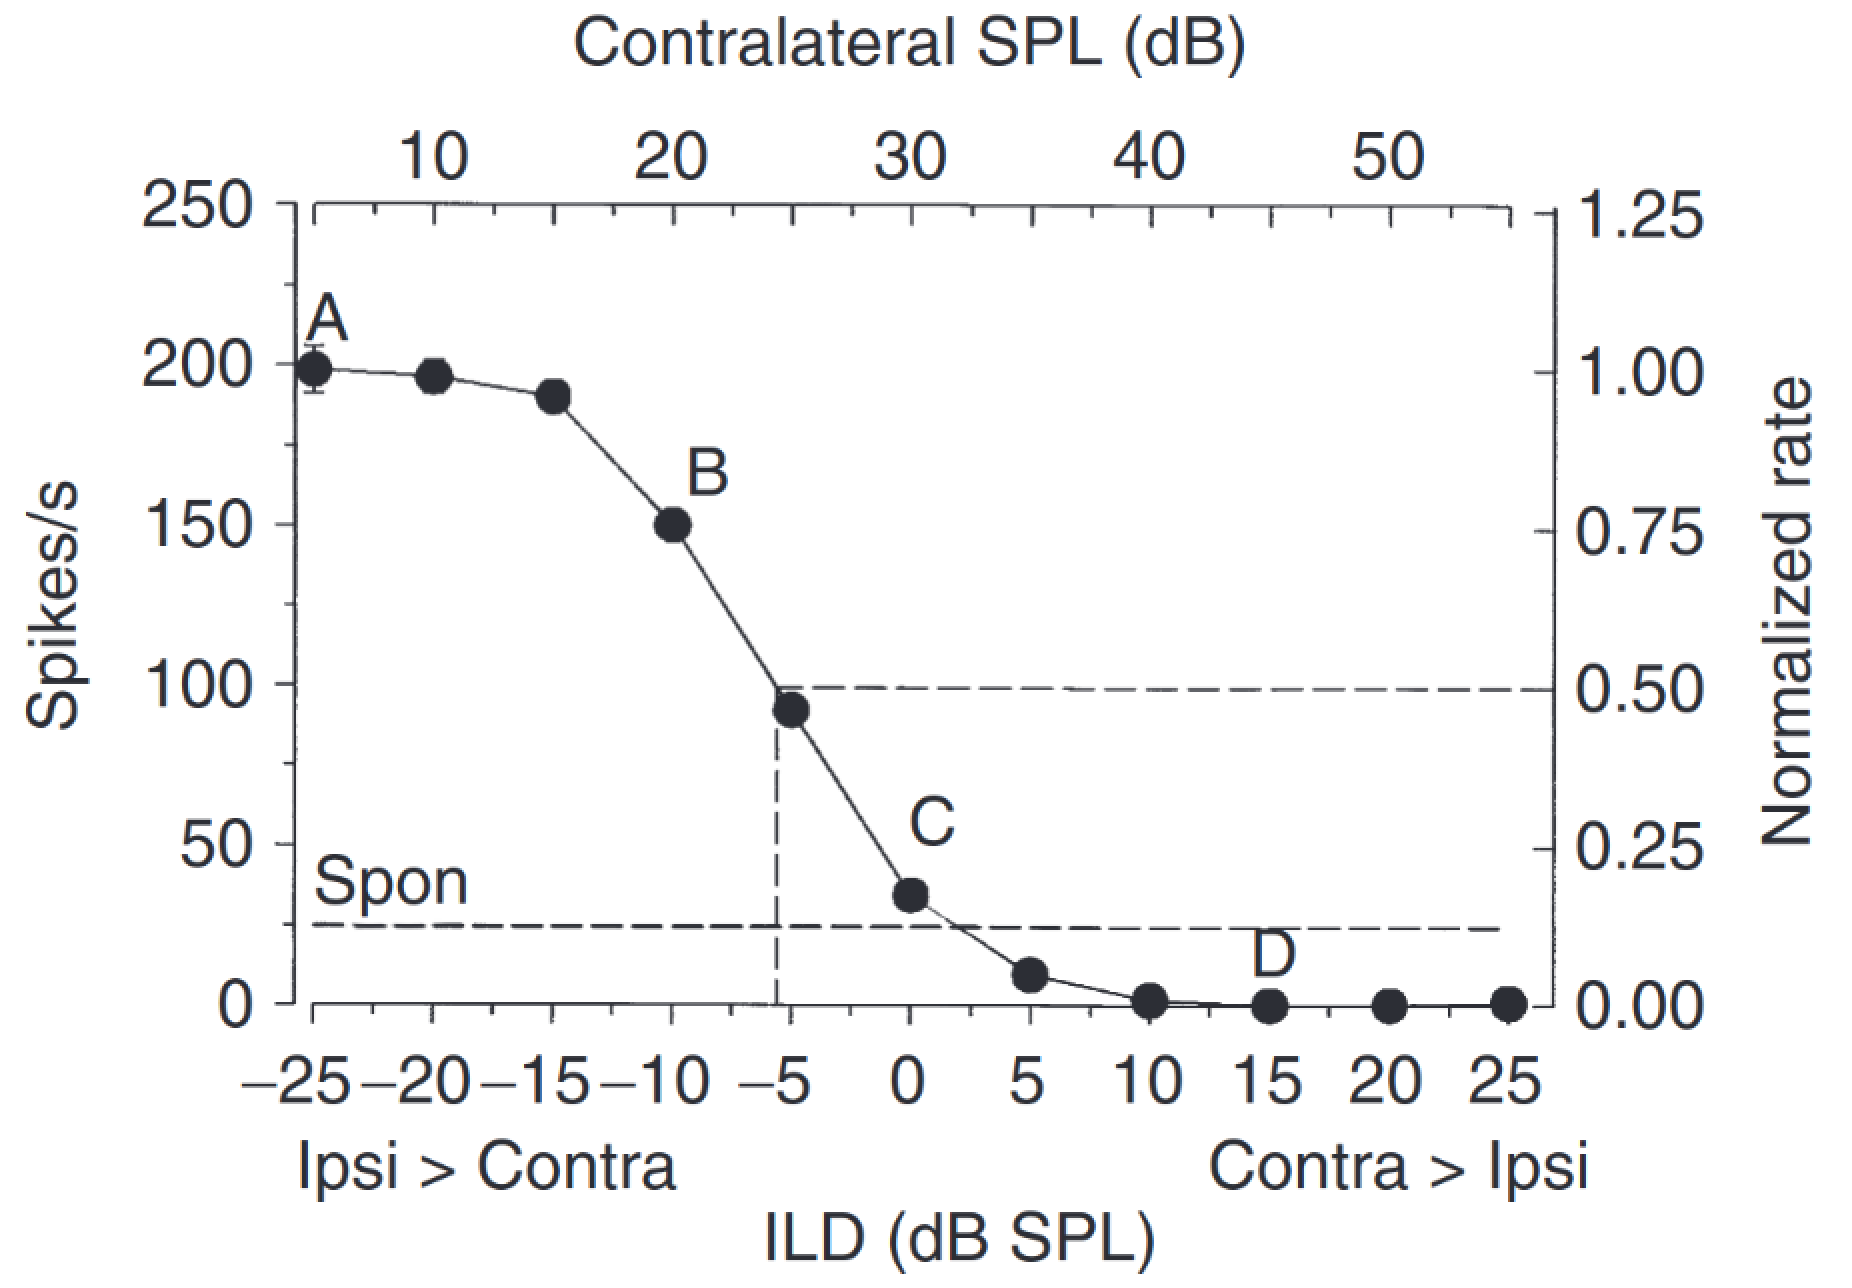
\includegraphics[width=0.48\linewidth]{Images/LSO-to-ILD.png}
    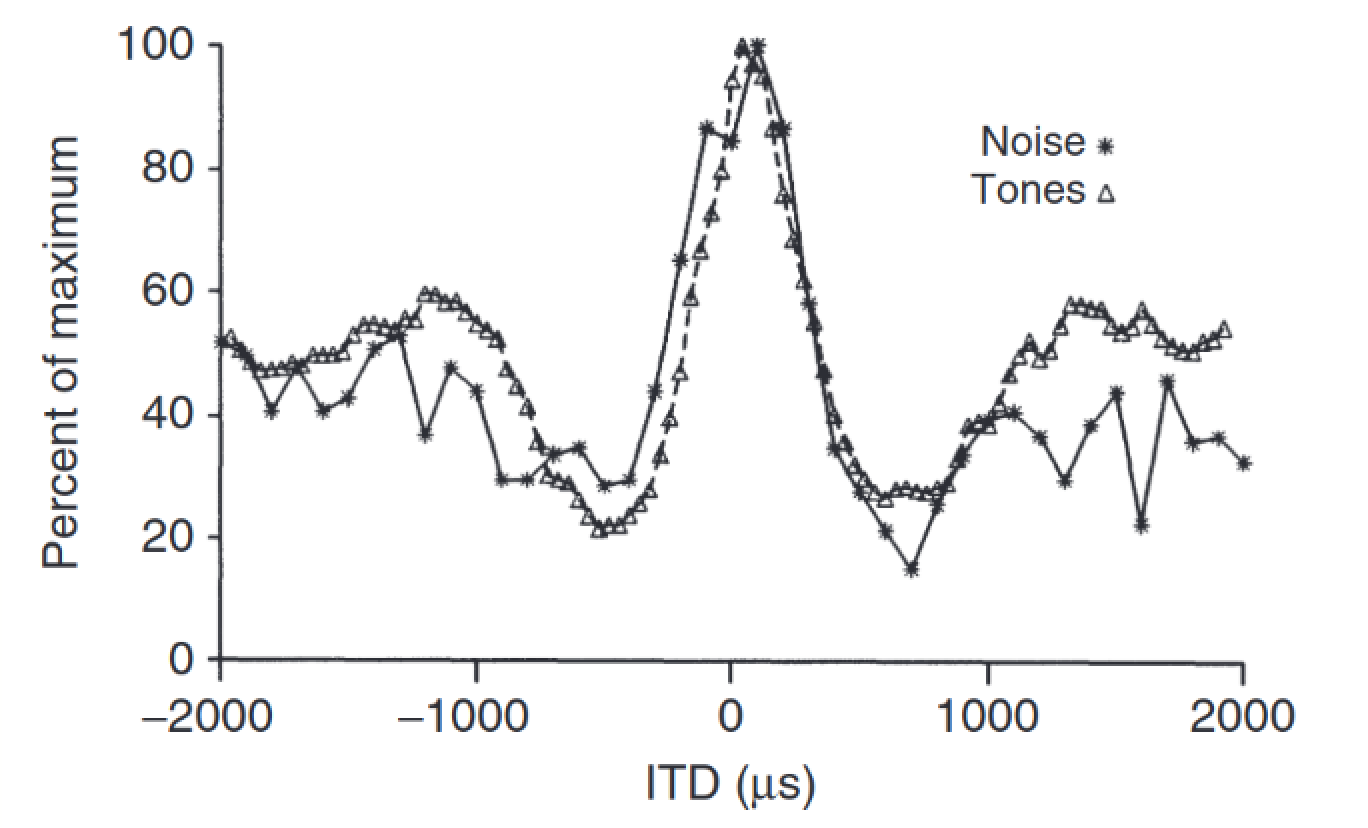
\includegraphics[width=0.48\linewidth]{Images/MSO-to-ITD.png}
    \caption{A plot showing the response of SOC nuclei to the cue they are most sensitive to, adapted from \cite{yinNeuralMechanismsBinaural2019}. On the left, the response of an LSO cell to an increasing contralateral level (increasing ILD). On the right, the response of an MSO cell to varying ITD. Notice the marked ipsilateral preference for the LSO, and contralateral-favoring response of the MSO.}
    \label{fig:lso-mso-expected}
\end{figure}

\paragraph{LSO}
Although there are four total inputs to the LSO, the two strongest inputs are the ones involved in sound localization: ipsilateral SBCs make excitatory synapses, while neurons from the MNTB form inhibitory synapses, which carry information from the contralateral GBCs. Most LSO axons then project to ipsi or contralateral ICC and DNLL; neurons projecting to the ICC innervate regions overlapping with those innervated by MSO neurons. 

\paragraph{MSO}
The MSO's principal cells have a strongly bipolar morphology, with dendrites stretched horizontally receiving bilateral inputs, both excitatory and inhibitory. The primary excitatory inputs to the MSO are from the SBCs of both sides, segregated on the two primary dendrites; instead, the primary inhibitory inputs come from the MNTB and LNTB of the side of the LSO, and synapse on the soma. The inhibition from the MNTB carries the signal from the contralateral ear. As mentioned, the MSO then projects to, among other nuclei, the IC, where the synaptic terminals synapse in regions overlapping \textit{ipsilateral} LSO terminals. Because of the small amplitude of responses, MSO recordings in vivo are difficult to obtain. The MSO presents a low input resistance and fast membrane time constant, requiring precise coincidence of subthreshold EPSPs for spiking. IPSPs have slower kinetics than excitatory inputs. An important characteristic is that stimulating ANFs, both contralaterally and ipsilaterally, causes an IPSP which arrives at the MSO before than the EPSP: this is suprising, because the excitatory path has a single synapse inbetween (ANF-SBC), while the inhibitory path has two synapses (ANF-GBC-MNTB).

\parspace
As we overviewed in \ref{sec:cues}, two main cues are involved in sound localization: interaural level disparities and interaural time disparities. The two nuclei we mentioned are the most likely candidates for where the processing of these cues happens.

\paragraph{Processing of ILDs}
Computing the ILD means subtracting the magnitude of the response of one ear from the other. As we mentioned, the LSO is excited by stimulation of the ipsilateral ear (from the SBCs) and inhibited by the contralateral ear (from the MNTB); this is very likely to be the main mechanism for processing ILDs. In addition, ILDs were shown to be the cue that LSO cells are most responsive to \cite{tollinCodingSpatialLocation2002}: as said in \ref{extra:hrtf_diff}, recording responses to free-field inputs is complicated, so most recordings are obtained using virtual acoustic spaces (VAS), partial HRTFs which only include some cues. The LSO is still tonotopically organized \cite{tsuchitaniFunctionalOrganizationLateral1977a}, so it is important to consider that the ILD the LSO can compute will still be dependent on frequency: a single location of the LSO receives intensity information of a small range of frequencies. The size of the range depends on 
\begin{inlinelist}
    \item how sensitive a specific BM region is to frequencies different from its CF (modeled with the gammatone bandwidth)
    \item how many BM regions are sensitive to each frequency (modeled with the density of gammatones and the ERB scale, see later)
    \item how many ANFs converge to a single SBC, so activity in different BM regions collapses to the same SBC (convergence) 
\end{inlinelist}. In the LSO, the latencies of inhibition and excitation, respectively contralateral and ipsilateral, are similar, even though inhibition requires an additional synapse through the MNTB.


\paragraph{Processing of ITDs}
Unlike the processing of ILD, the processing of ITDs is less understood. This may be in part because the nucleus that is believed to process them is difficult to record from: it is narrow, sometimes one or two cells thick; its action potentials are small; the region is flooded with phase-locked potentials from the auditory chain we've reviewed so far \cite{scottPosthearingDevelopmentalRefinement2005a}.  Multiple strategies have been proposed, but the precursor is a model presented by Jeffress in 1948. This model assumes that ITDs are processed by an array of simple coincidence detectors (neurons that respond maximally when the two inputs arrive simultaneously), wired with progressively longer delay lines (based on axonal length) that generate internal delays. Then, the coincidence detector that fires maximally will represent the current ITD, generating an internal map of ITDs (see \ref{fig:jeffress}).
\begin{figure}[H]
    \centering
    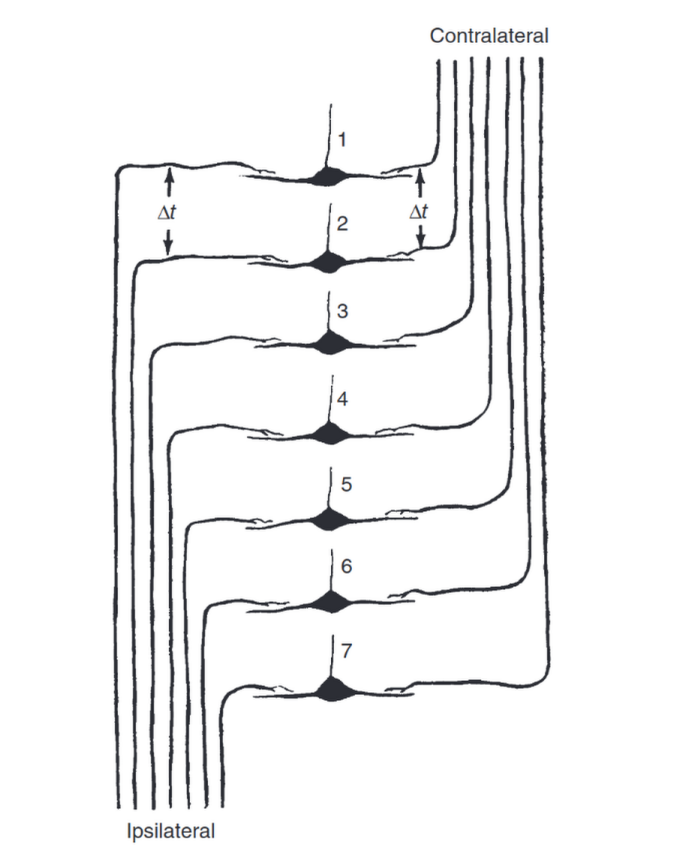
\includegraphics[width=0.5\linewidth]{Images/yin-1526.png}
    \caption{The Jeffress model to recognize ITDs, from \cite{yinNeuralMechanismsBinaural2019}}.
    \label{fig:jeffress}
\end{figure}

If we consider the MSO to be the site of this model, its first assumption is that precise timing information is available to the MSO: this assumption is correct, as the mechanism of phase-locking can, within the frequency range in which it functions, relay precise information about the phase (and hence the timing) of both sides. In addition, SBCs and GBCs enhance ANFs phase-locking properties \cite{jorisEnhancementNeuralSynchronization1994a}. The role of the coincidence detector that the Jeffress model would assign to MSO is also reasonably accurate: it responds maximally when inputs arrive almost coincidentally. This difference from the exact coincidence varies among cells and makes for a cyclical response pattern modulated by frequency. ITD curves for the same neuron at various frequencies share a characteristic delay (CD) at which they all have the same relative amplitude. If the conduction time were constant with respect to the frequency of the input, CDs would only be at peaks or troughs, but this is not the case: while most cells in the MSO have CDs when all curves are at their peak (thus called peak-type cells, figure A), others have their CDs at different phases (non-peak type).
\begin{figure}[H]
    \centering
    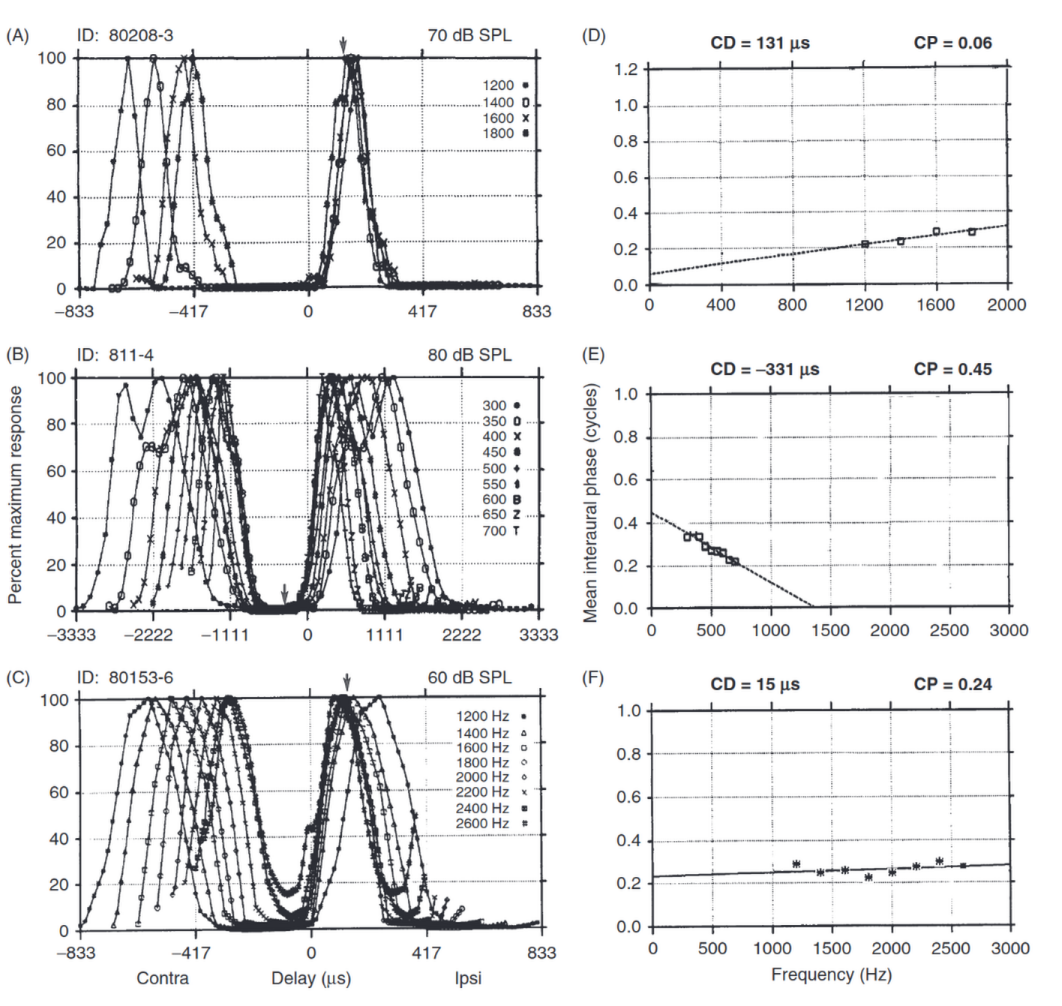
\includegraphics[width=0.5\linewidth]{Images/yin-1530.png}
    \caption{Responses from the ICC, used as a proxy for the MSO, showing the different types of cells. On the right, the interaural phase vs frequency plots. ITD curves are normalized. From \cite{yinNeuralMechanismsBinaural2019}}
    % \label{fig:enter-label}
\end{figure}

This is where the Jeffress model shows its weaknesses: 
\begin{inlinelist}
    \item only peak-type cells make sense in a Jeffress interpretation
    \item\label{jeff:weak2} the model would predict neurons to show a range of internal delays, distributed on the range of possible ITDs
    \item\label{jeff:weak3} for the cause to be the axonal delay due to its length, these delays would need to be distributed spatially
\end{inlinelist}. Consequence \ref{jeff:weak2} would expect delays to correspond to the physiological ITD range. Instead, evidence in cat \cite{yinInterauralTimeSensitivity1990a} and guinea pig \cite{mcalpineNeuralCodeLowfrequency2001} IC (used as a proxy for the MSO) show a similar range despite much different head sizes. In addition, although axonal length varied, a re-analysis of past data \cite{karinoAxonalBranchingPatterns2011} found two important inconsistencies with consequence \ref{jeff:weak3}: the anatomical data could not explain the range of optimal delays (OD, maximal response ITD), and there was an inverse relationship with CF (large ODs only in low frequencies, and OD decreased as frequency increased \cite{mcalpineNeuralCodeLowfrequency2001}\footnote{While the trend was confirmed in other animals, the lack of small ODs in low frequencies wasn't.}) which would not be compatible with a delay line mechanism (but more compatible with an internal phase-shifting mechanism). We are left with two important questions, to which there have been multiple plausible answers but no definitive ones:
\begin{itemize}
    \item \textbf{How are internal delays generated?} There are two main lines of research;
    \begin{inlinelist}
        \item \textit{Cochlear delays}: connecting locations in the basilar membrane that resonate at different frequencies, one could make use of the relatively slow traveling wave to generate delays in the cochlea itself \cite{yinNeuralMechanismsBinaural2019}; this theory has very limited physiological tests, and to correspond to physiological data, where CDs are biased toward the contralateral ear, errors would need to be biased as well, with the contralateral CF being lower than the ipsilateral CF.
        \item \textit{Inhibition-driven}\label{myoga}: as we've mentioned, several factors suggest an essential role for inhibition; among them: the bipolar nature of MSO neurons; two different sources of inhibition, one from each ear; inhibition is phase locked; the synapse driving the contralateral inhibition (the calyx of Held, from GBCs to MNTB) is the largest known synapse; inhibition was shown to be faster (in arrival time) than the corresponding excitation; blocking inhibition shifts ODs towards 0ms \cite{brandPreciseInhibitionEssential2002a}. Yet, the mechanism behind the role of inhibition is unknown; one proposal was that MNTB-carried inhibition delays the excitatory EPSP \cite{brandPreciseInhibitionEssential2002a}; in one later study, inhibition was found not to have any effect on ITD tuning \cite{robertsMechanisticUnderstandingRole2013a}, while in another one preceding inhibition could not be measured \cite{vanderheijdenDirectionalHearingLinear2013}. A following proposal \cite{myogaGlycinergicInhibitionTunes2014} explored the effect of various time deltas between each pair of excitation and inhibition from the same side and found that the ITD of maximal response could be shifted significantly by changing these two parameters, highlighting the relevancy of both inhibition sources.
    \end{inlinelist}
    \item \textbf{What is their relationship with ITDs?} The relationship between internal delays, optimal delays, and species ITD is still unclear. As mentioned, species with different head widths (hence different maximal ITD) do not show significant differences in the distribution of ODs; in addition, OD distribution is not restricted to the physiological range of the species. This has led researchers to consider the possibility that ODs are not distributed to respond maximally to specific ITDs but to have the maximal change in firing rate over the species physiological range for ITDs \cite{mcalpineNeuralCodeLowfrequency2001a}\cite{harperOptimalNeuralPopulation2004}. This led to the \textit{two-channel model}, according to which the activity of LSO and MSO can be combined, with opposite maximal response points (\ref{fig:twochann}). The original formulation of the two-channel model (encompassing the integration of LSO and MSO) is incompatible with several results\footnote{See \cite{yinNeuralMechanismsBinaural2019} for details; as examples: unilateral midbrain lesions leave most subjects with unaffected ipsilateral localization ability but impaired in contralateral space; the variety in MSO ODs, considered noise for a two-channel model, and the closeness to zero ITD are important features for interaural decorrelation, very acute in humans}, with some authors \cite{grotheNaturalHistorySound2014} now requalifying the MSO as focused on sound segregation, due to its context-dependant modulation.
\end{itemize}

\begin{figure}
    \centering
    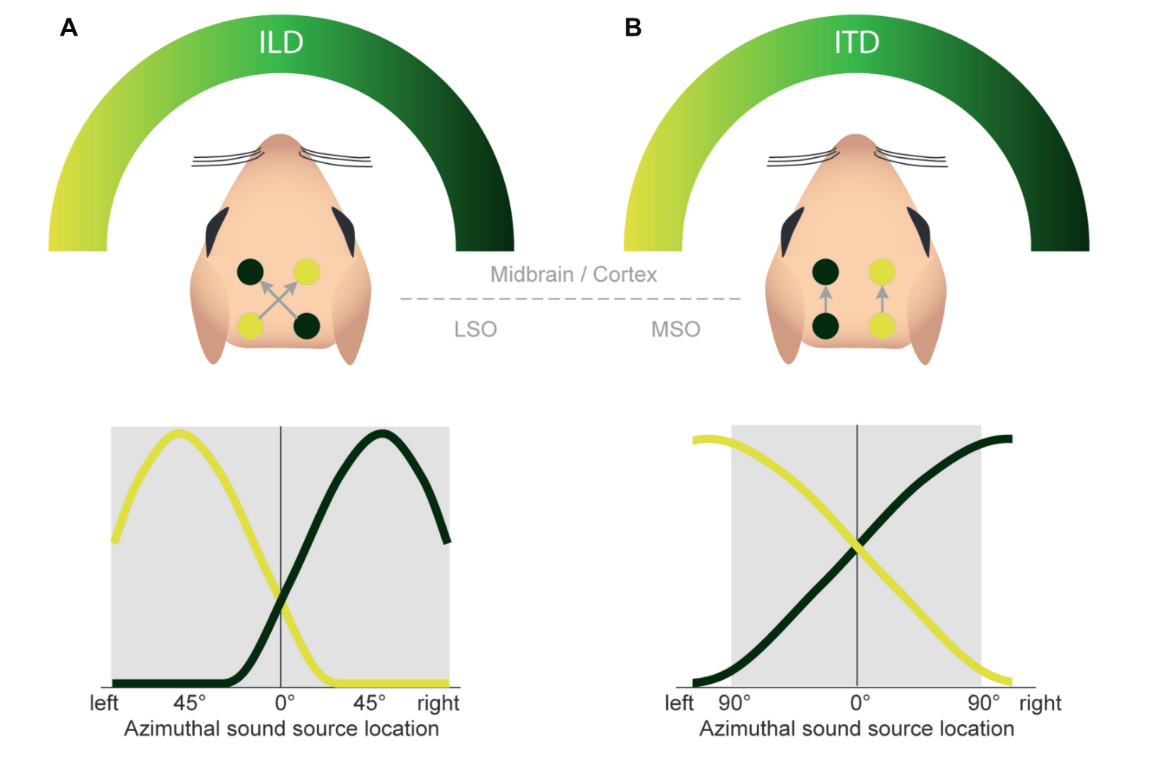
\includegraphics[width=0.5\linewidth]{Images/two_channel_model.png}
    \caption{A diagram showing how LSO and MSO inputs converge to higher centers, in the two-channel model. From \cite{grotheMechanismsSoundLocalization2010}}
    \label{fig:twochann}
\end{figure}

\paragraph{Inferior Colliculus}\label{sec:ic-theory}
Finally, we examine some properties of the last site of convergence we will cover, the inferior colliculus (IC). Although the IC comprises three regions - central nucleus, dorsal cortex, and external cortex - the central nucleus (ICC) is the primary region of interest for auditory processing, together with the brachium of the IC (BIN). The ICC receives input from both of the SON nuclei discussed so far, LSO and MSO, in addition to other sources; specifically, each IC receives input from ipsilateral MSO and contralateral LSO. These synapses are mostly excitatory, forming an EE scheme (excitatory-excitatory) \cite{grotheMechanismsSoundLocalization2010}. Cells in the ICC have shown varying properties and classified accordingly: type V units, sensitive to ITDs, type I units, sensitive to ILDs, and type IV units, resembling neurons in the dorsal cochlea nucleus, which processes spectral cues. Some results \cite{sleeAlignmentSoundLocalization2014} suggest that most cue integration happens at the BIN, but the same authors found that most neurons in the BIN responded strongly to ILDs, while the contribution of ITDs was weak \cite{sleeLinearProcessingInteraural2013}.
In addition, evidence for a spatial map has not been found, and some results \cite{seshagiriResponsePropertiesNeighboring2007} suggest that auditory cues may remain more segregated than previously thought. Overall, the literature does not definitively answer whether and how auditory cues are integrated above the SOC.

\newpage


\section{Aim of the Thesis}
Given the state of research around sound localization, this work improves an existing, simplified, neural-only computational model \cite{santisComputationalModelMammalian}, with three main objectives:
\begin{enumerate}
    \item\label{obj:bioplaus} Improve the bioplausibility of the existing model by:
    \begin{enumerate}
        \item Implementing peripheral sections at three levels of bioplausibility:
        \begin{inlinelist}
            \item\label{obj:coch-pulse} \textit{Pulse packet} (see \ref{sec:pulsepacket})
            \item\label{obj:coch-gamm} \textit{Gammatone-based}
            \item\label{obj:coch-tc} \textit{Tan-Carney based, bioplausible mammalian cochlea}
        \end{inlinelist}
        \item Evaluating the effect of these peripheral sections on SOC nuclei
    \end{enumerate}
    \item\label{obj:mso} Use Myoga's principles to produce a contralateral-favoring MSO without the use of dedicated delay lines
    \item\label{obj:icc} Consider an EE (contralateral LSO and ipsilateral MSO) scheme for auditory cue integration above the SOC with a synthesized IC model and quantitatively evaluate it on three metrics:
    \begin{enumerate}
        \item \textit{Zero-degree accuracy}: Since behavioral results show no difference between right and left azimuthal localization accuracy, the center point (zero degrees) should show equal activation in both populations;
        \item \textit{Increased sensitivity around zero}: JND is lowest in humans around zero azimuth. Hence, a steeper curve is an improvement;
        \item \textit{Range}: Difference between maximum and minimum total population spike index to maximize the difference in lateralization.
    \end{enumerate}
\end{enumerate}




\section{Methods}
This project was split into two sections: the first focused on increasing the bioplausibility of the peripheral system, and the second increased the bioplausibility of the neural processing. As such, the needs of the two sections varied substantively, and different strategies were adopted. The modeling of the peripheral section, from the sound to the spiking output of ANFs, was implemented using Brian2Hears, an extension to Brian 2. The modeling of the central nervous system was developed using the NEST simulator framework. This section will introduce the two, explain the differences, detail how the simulation was set up, and define how we will test its results. We will take a sequential approach to mirror the biological explanation, starting with the peripheral simulation and then explaining the central processing.

\parspace
Considering what has been mentioned so far, we will use these conventions:
\begin{itemize}
    \item Only consider front-facing angles, where zero degrees represents the center, -90 is extreme left, and +90 is extreme right.
    \item Only consider human application: all ITDs shown will use a human range, and, where this is not specified, the diameter of the human head will be approximated as \qty{22}{\centi\meter}
\end{itemize} 

\subsection{Peripheral Modeling}
\subsubsection{Simulator}
We modeled the bioplausible peripheral stages using Brian 2 Hears \cite{fontaineBrianHearsOnline2011}. Brian 2 Hears is an extension for Brian 2 \cite{stimbergBrian2Intuitive2019} to enable auditory modeling; it is also usable as standalone, and we will use it both ways. Brian 2 Hears and Brian 2 are both written in Python. As we will see in section WRITEME, one important weakness of Brian 2 Hears is that it is inherently single-threaded: although simulations can be run in parallel, a single simulation cannot be sped up by parallel computation.

Using Brian 2 Hears, we implemented two peripheral sections at different levels of bioplausibility. As we mentioned in section~\ref{sec:model-periph}, components of the peripheral auditory system can be modeled using different strategies; using Brian 2 Hears means utilizing digital filters to approximate the behavior of each component. We also detailed how modelers must evaluate the complexity/bioplausibility tradeoff for each component: this would have resulted in far too many models to test end evaluate, so we decided to limit the choice to a simple gammatone model and the more advanced Tan-Carney model \cite{tanPhenomenologicalModelResponses2003}. We also avoided optimizing model parameters, and used literature values.

Figure \ref{fig:block-periph-general} shows the pathway common to all peripheral models. First, a sound, together with its location, is filtered through an HRTF, obtaining the filtered sounds as they arrive in the acoustic canal of the two ears. Then, each ear goes through peripheral processing, which varies among the different models we tested, and causes an ANF spiking pattern. The ANF spike trains are the final result of the peripheral processing pipeline.

\begin{figure}
        \centering
        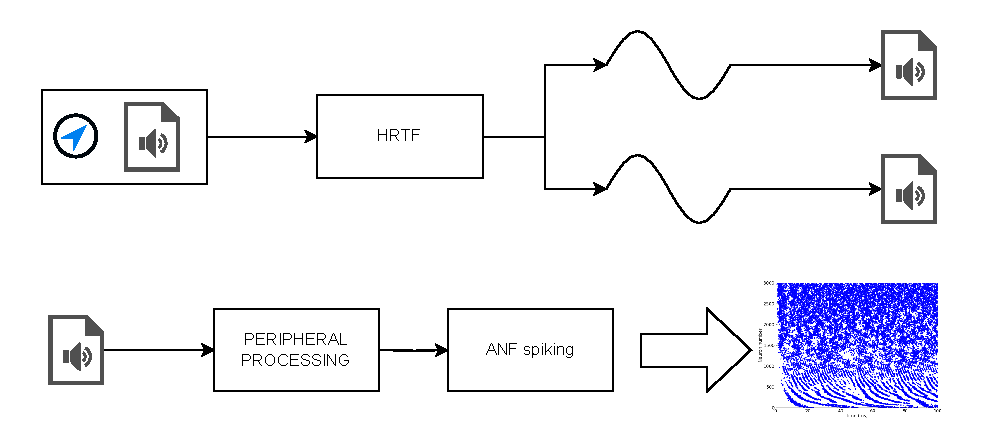
\includegraphics[width=1\linewidth]{Images/block-HRTF-cochlea-general.pdf}
        \caption{Block scheme for auditory peripheral processing}
        \label{fig:block-periph-general}
\end{figure}

\subsubsection{Gammatone}
The processing of the Gammatone peripheral model is articulated in these steps:
\begin{enumerate}
    \item \textit{HRTF}: the sound is filtered through an HRTF to obtain the two inputs to each ear. We used the IRCAM LISTEN \cite{LISTENHRTFDATABASE} database. This early database is well-integrated with brian2hears\footnote{Its recording setup was a single-microphone, single-speaker setup, with the speak attached to a metallic u-shaped supporting structure with two dimensions of movement.}. This limits us to \ang{15} increments in azimuthal position (13 positions). This process is common to all our peripheral models.
    \item \textit{CF spacing}: as we mentioned, CFs lower logarithmically along the BM. This organization is approximated using the center frequencies of the ERB scale \cite{zwickerAnalyticalExpressionsCriticalband1980a}. We used 3500 IHCs, as in the human cochlea \cite{ashmoreCochlearOuterHair2008}.
    \item \textit{Gammatone}: then, for each ear, CFs become the center frequencies of 3500 gammatone filters in a filter bank. The sound is filtered by the filter bank in each ear, modeling how inner hair cells are engaged depending on frequency.
    \item \textit{Cochlea}: After the gammatone filterbank, the active component of the cochlea is modeled with a cube root power law, the simplest estimate \cite{stevensPsychophysicalLaw1957} of the active cochlea compression.
    \item \textit{Current transformation}: Each filtered response will now be interpreted as a current raising the cell voltage of an IHC cell. To do that, it will be rectified (half wave). This will be analogous to the mechanical movement of the IHC opening and closing ion channels. The current is then multiplied by an appropriate scalar (15).
    \item \textit{ANFs}: The current then raises the voltage of IHC cells, causing it to release more neurotransmitters in the synaptic cleft, making the ANFs spike. Effectively, the IHC and ANF are modeled as a single unit whose inner voltage is raised by the current until the spike threshold is reached. This is where noise is included in the output, summed to a simple leaky integrate-and-fire model. This neuron model includes a refractory period: when the refractory period is set at \qty{1}{\milli\second}, it will not be able to fire faster than \qty{1}{\kilo\hertz}. This can be used to model effective phase locking at low frequencies and the inability to cope with high frequencies.
\end{enumerate}

\parspace
This results in a model which shows phase locking (particularly obvious at low frequencies), but will have limited biological plausibility, showing no adaptation (as it has no concept of vesicle availability), no tone interaction, approximate IHC frequency response and the other drawbacks explained in section~\ref{sec:model-periph}. At the same time, most of these features are not strictly related to sound localization. As this model is not attributed to a specific author, we experimented with noise level. This noise models the spontaneous rate, not the noise in the sound. All effects on the sound are carried by the HRTF as if our experiment \textit{in silico} were happening in an anechoic chamber.

\begin{figure}[H]
    \centering
    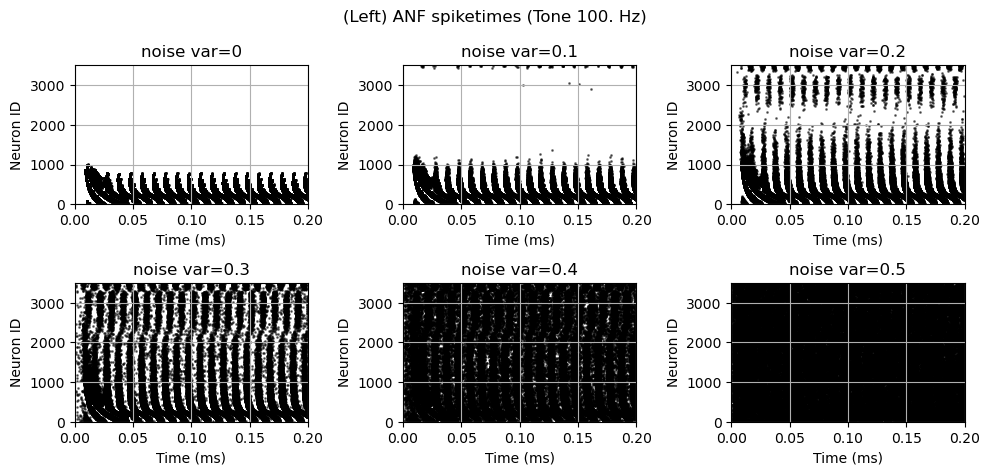
\includegraphics[width=1\linewidth]{Images/gammatone-noise.png}
    \caption{ANF responses with increasing noise variance.}
    \label{fig:anf-noise}
\end{figure}

\subsubsection{Tan Carney}
The processing of the Tan Carney cochlea traces the steps of the gammatone-based cochlea, with some changes. The structure follows the original Tan Carney paper \cite{tanPhenomenologicalModelResponses2003}:
\begin{enumerate}
    \item \textit{HRTF}.
    \item \textit{Resampling}: Because of how the Tan Carney cochlea is implemented, it requires inputs with a sample rate of \qty{50}{\kilo\hertz}, but HRTFs use a more standard \qty{44.1}{\kilo\hertz} sample rate. So, sounds are first processed through the unchanged HRTF and then resampled to match the requirements of the following steps.
    \item \textit{CF spacing}.
    \item \textit{Middle Ear}: To model the gain introduced by the middle ear, the original paper uses a linear bandpass filter based on middle ear frequency response reported by Rosowsky \cite{rosowskiModelsExternalMiddleEar1996}.
    \item\label{met:tancarney-cochlea} \textit{Cochlea}: After this, the Tan Carney cochlea substitutes the gammatone filterbank: it uses two paths, a time-varying bandpass filter for the signal and a nonlinear control path to account for compressive nonlinearity in the BM.
    \item \textit{IHC Synapse}: Finally, the IHC and the IHC-ANF synapse are modeled using the Zhang \cite{zhangPhenomenologicalModelResponses2001} model, featuring a saturating low-pass filter for the IHC and the three-store model we saw in Paragraph \ref{bio-IHC}.
\end{enumerate}

It is important to note that this model was not initially planned for the human cochlea: the data used to fit the parameters of the signal path mentioned in \ref{met:tancarney-cochlea} used the available data of low-frequency cat ANF. Still, the low availability of high-CF cat ANFs is irrelevant for human application, as human hearing tops out around \qty{20}{\kilo\hertz}. As the model aims to reproduce responses from ANFs with high spontaneous rates, we do not need to add any additional noise \cite{tanPhenomenologicalModelResponses2003}.

\subsubsection{Pulse Packets}\label{sec:pulsepacket}
The last cochlea we designed is at the opposite end of bio-plausibility and is handmade to have the cleanest possible inputs to our neural processing section. It serves as our control and shows the limit of what our neural processing section can produce with perfect inputs. It uses some basic features of NEST Simulator, the simulator for our neural processing section, which we introduce more completely in Section \ref{met:nest}. 

CFs are distributed logarithmically. We use pulse packet generators to produce a spike train with Gaussian pulse packets centered around the exact phase-locking time. A Gaussian pulsepacket is a set number of spikes (depending on the ILD), with normal distributed random displacements from the center time. The standard deviation of spike times within each pulse is a simulation parameter. We obtain two series of pulse packet generators, one series for each ear; between them, center times differ by an ITD determined from the angle with the formula of 

\begin{lstlisting}[language=Python]
    delta_x = w_head * np.sin(np.deg2rad(angle))
    itd = np.round(1000 * delta_x/v_sound, 2) # ms
\end{lstlisting}
To ensure proper signal propagation, we involve 10 ANFs before and 10 ANFs after the neuron with each CF, whose activity (spikes per pulse) is modulated by a Gaussian profile of amplitudes.
To maintain the structure of the other peripheral models, the simulation using these pulse packet generators is run, and the resulting spike times are saved. They will then be loaded as inputs to the neural processing section.

\subsection{Neural Processing}
Once the peripheral model has determined the ANF spiking patterns, they are saved into a binary file to avoid re-generation for every run. Then, spike generators are created using the ANF spiking patterns, which will be the inputs for the neural processing section.

\subsubsection{Simulator}\label{met:nest}
For the neural processing section, we decided to use NEST Simulator \cite{gewaltigNESTNEuralSimulation2007}. Like Brian 2, NEST allows the modeling of Spiking Neural Networks, enabling experiments to be performed \textit{in silico}. We interacted with the NEST simulator using PyNEST. This Python interface serves as an API layer translating Python requests into code made for a Simulation Language Interpreter (SLI), which finally controls the Nest Kernel, written in C++. One significant advantage of NEST was the availability of built-in thread parallelism, which enabled a substantial speedup.
All simulations were run on a personal laptop, using an AMD Ryzen™ 7 7840U (up to 5.1GHz, 8-core/16-thread) with 32GB DDR5 RAM memory\footnote{The RAM was crucial, as simulations could take as much as 15GB of RAM}, on OpenSUSE Tumbleweed.

\subsubsection{Network Structure}
Because the model was inherited from a previous work \cite{santisComputationalModelMammalian}, we will only outline the network structure and highlight the changes that were made to improve its bio-plausibility.


\begin{table}[H]
\centering
\begin{tabular}{|l|l|l|c|}
\hline
\rowcolor{bluePoli!40}
\begin{tabular}[c]{@{}l@{}}Cell Type\end{tabular} & Model & Convergence & Numerosity \\
\hline
ANFs & 
\begin{tabular}[c]{@{}l@{}}parrot\_neuron\\(devices that reproduce \\peripheral model output)\end{tabular} & 
\begin{tabular}[c]{@{}l@{}}4 : 1 to SBCs\\20 : 1 to GBCs\end{tabular} & 35000 \\
\hline
SBCs & iaf\_cond\_alpha & 
\begin{tabular}[c]{@{}l@{}}5 : 1 to LSO PCs\\5 : 1 to MSO PCs\end{tabular} & 8750 \\
\hline
GBCs & iaf\_cond\_alpha & 
\begin{tabular}[c]{@{}l@{}}1 : 1 to LNTBC\\1 : 1 to MNTBC\end{tabular} & 1750 \\
\hline
LNTB & iaf\_cond\_alpha & 1 : 1 to MSO PCs & 1750 \\
\hline
MNTB & iaf\_cond\_alpha & 
\begin{tabular}[c]{@{}l@{}}1 : 1 to LSO PCs\\1 : 1 to MSO PCs\end{tabular} & 1750 \\
\hline
MSO & iaf\_cond\_beta & 1 : 1 to IC & 1750 \\
\hline
LSO & iaf\_cond\_alpha & 1 : 1 to IC & 1750 \\
\hline
IC & iaf\_cond\_alpha & - & 1750 \\
\hline
\end{tabular}
\end{table}

\paragraph{Membrane time constant}
An important step for realism was moving to a more realistic membrane time constant ($\tau_m$). The membrane time constant is an important property of neurons, which measures how quickly the membrane potential changes to respond to input currents and decay back to rest potential. In our application, the membrane time constant is especially relevant: as mentioned in Section \ref{sec:bg}, all cells involved in the auditory pathway have exceptionally fast time constants. In NEST, the membrane time constant is not a direct parameter but is determined from membrane capacity ($C_m$) and leak conductance ($g_L$): $\tau = C_m / g_L$. The existing model, to ensure sufficiently quick membrane time constants, used extremely low membrane capacities (\qty{1}{\pico\farad}), which lead to an unrealistic membrane time constant ($=\qty{0.06}{\milli\second}$). A realistic range \cite{caoVoltagesensitiveConductancesBushy2007} of $C_m$ for bushy cells is \qtyrange{2}{0.6}{\milli\second}. This short time constant allowed for very fast response to inputs, precise temporal processing, and great ability to track input changes, but meant that 
\begin{inlinelist}
    \item Bushy cell populations were able to phase lock to excessively high frequencies;
    \item As soon as noisier, more realistic cochleas were used, the temporal window for coincident spikes, which triggered spiking, immediately became too small.
\end{inlinelist}

We moved to a higher membrane capacitance and a higher (but lower proportionally) leak conductance to increase the membrane time constant to a reasonable range. The high leak conductance simulates the fast ion channels present throughout the auditory pathway. Table~\ref{tab:pop-cap-leak} collects the membrane capacitance and leak conductance.
\begin{table}[H]
    \centering
    \begin{tabular}{|l|c|c|}
        \hline
        \rowcolor{bluePoli!40}
        Population & Membrane Capacitance ($C_m$, pF) & Leak Conductance ($g_L$, nS) \\
        \hline
        SBC & 15 & 40 \\
        \hline
        GBC & 15 & 25 \\
        \hline
        MNTBC & 15 & 25 \\
        \hline
        LNTBC & 15 & 25 \\
        \hline
        MSO & 20 & 80 \\
        \hline
        LSO & 30 & 20 \\
        \hline
        ICC & 20 & 20 \\
        \hline
    \end{tabular}
    \caption{Membrane capacitance ($C_m$) and leak conductance ($g_L$) values for the different neuron populations.}
    \label{tab:pop-cap-leak}
\end{table}

A side effect of increasing the membrane time constant was that pulse-packet generators were unable to generate spikes in the MSO. 

\paragraph{Timing}
As mentioned in \ref{myoga}, Myoga et al. in \cite{myogaGlycinergicInhibitionTunes2014} propose one plausible theory for how internal delays are generated, which does not make use of delay lines organized by frequency or cochlear delays. By delivering inhibition modeled on recorded IPSP to Mongolian gerbil brain slices, they found that inhibition dynamically shifts the timing at which excitation reaches its maximum voltage. In turn, when using bilateral inhibition and bilateral excitation, as with the bipolar MSO neuron, the coincidence detection feature of MSO neurons is modulated, allowing the researchers to shift the best ITD from zero to a range of $\pm \qty{200}{\micro\second}$. To use this result, we first verified its applicability to the simple \lstinline{iaf_cond_beta} model; in addition to the coincidence detection tuning, we also replicated its efficacy on higher frequencies. Once we confirmed its applicability, we included these findings in our model, using delays that account for the delay due to synaptic integration. To maximize contralateral bias, we used the largest delays shown in \cite{myogaGlycinergicInhibitionTunes2014}, $\Delta T_{inhi}=0.2$ (difference in time of arrival between ipsilateral excitation and ipsilateral inhibition) and $\Delta T_{inhc}=-0.4$ (difference in time of arrival between ipsilateral excitation and ipsilateral inhibition):


\begin{table}[H]
\centering
\begin{tabular}{|l|l|c|c|}
\hline
\rowcolor{bluePoli!40}
\begin{tabular}[c]{@{}l@{}}Source pop\end{tabular} & Dest pop & Formula & Delay (\qty{}{\milli\second}) \\
\hline
GBCs & MNTBC & -- & 0.45 \\
\hline
GBCs & LNTBC & -- & 0.45 \\
\hline
SBCs & MSO (ipsilateral) & -- & 2 \\
\hline
SBCs & MSO (contralateral) & -- & 2 \\
\hline
LNTB & MSO & 1.44 + $\Delta T_{inhi}$ & 1.64 \\
\hline
MNTB & MSO & 1.44 + $\Delta T_{inhc}$ & 1.04 \\
\hline
\end{tabular}
\caption{Timings of connections between populations}
\end{table}

We also verified Myoga's values in our complete network, shown in Figure~\ref{fig:myoga-on-big-net}. In the top plot, the MSO responds maximally to contralateral sounds, while in the bottom plot, the MSO responds maximally to ipsilateral sounds. All other parameters were kept constant. The middle plot shows a modest effect from a slight delay change.

\begin{figure}[H]
    \centering
    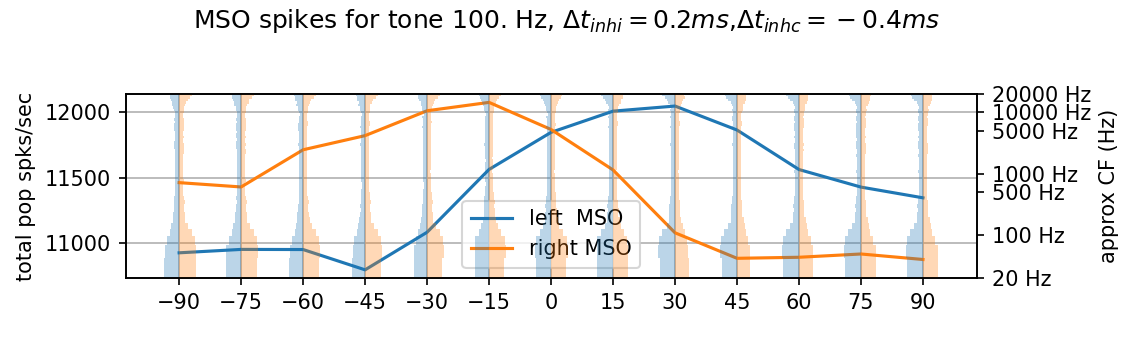
\includegraphics[width=0.5\linewidth]{Images/msonormal.png}
    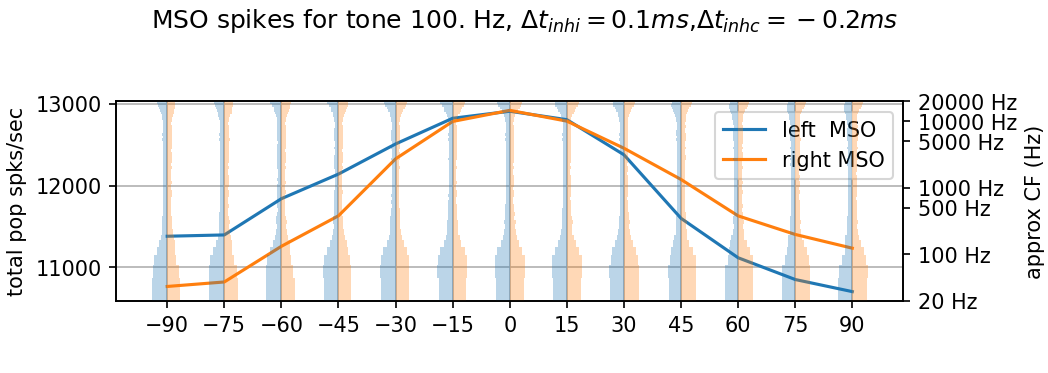
\includegraphics[width=0.5\linewidth]{Images/msocenter.png}
    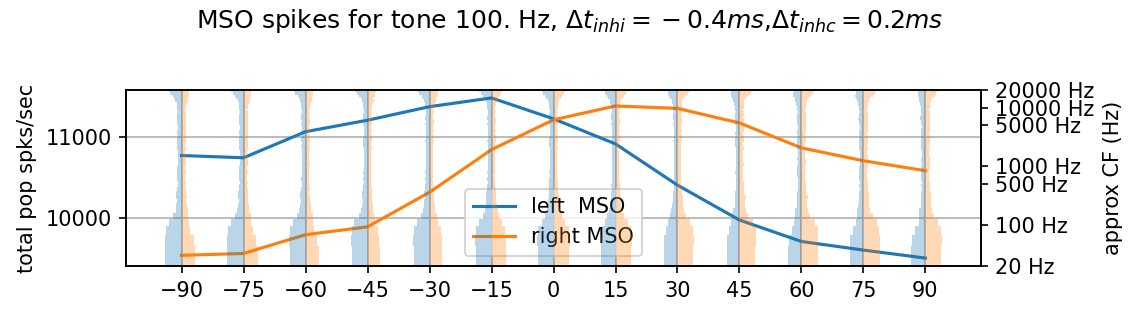
\includegraphics[width=0.5\linewidth]{Images/msoabnormal.png}
    \caption{The effect of changing relative arrival times of inhibition from the two sides relative to the excitation arrival times.}
    \label{fig:myoga-on-big-net}
\end{figure}

\paragraph{Weights}

In Table~\ref{tab:connections-weights}, we show the weights used for all synaptic connections in the network.
\begin{table}[h]
\centering
\begin{tabular}{|l|l|r|}
\hline
\rowcolor{bluePoli!40}
Source population & Destination population & Synaptic Weight \\
\hline
ANFs & SBCs & 35.0 \\
ANFs & GBCs & 7.0 \\
\hline
GBCs & LNTBCs & 20.0 \\
GBCs & MNTBCs & 30.0 \\
SBCs & LSO & 10.0 \\
MNTBCs & LSO & -10.0 \\
SBCs & MSO & 9.0 \\
MNTBCs & MSO & -40.0 \\
LNTBCs & MSO & -40.0 \\
\hline
MSO & IC & 20.0 \\
LSO & IC & 20.0 \\
\hline
\end{tabular}
\caption{Synaptic weights between populations}
\label{tab:connections-weights}
\end{table}


\subsection{Testing}
Due to the multilevel aim of this work, testing was done at multiple levels. Here, we will show what our testing procedure was for each level of processing, highlighting the most relevant metrics.

\subsubsection{Peripheral processing}
In the peripheral section, we evaluated results at two points: first, the effect of HRTFs on sound, and then the quality and bio plausibility of ANF spikes by each of our cochleas.

\paragraph{HRTF}
To evaluate the effect of HRTFs on sounds, rather than plotting the response or the spectrum of the resulting binaural sound, we cast its effect into what our investigation was based on so far: interaural cues. This was especially relevant because of the azimuthal focus of our work. Since we preferred examining tones, as these allowed us to investigate a narrow band of neuronal fibers, ILD was measured as the maximum of the difference in the spectrum of right and left sounds. Because of noise and recording artifacts, measuring ITD needed to account for minor variations before the onset of the actual transformed sound, so we profiled the silence and only considered the beginning of the sound from the first sampled value that exceeded a threshold proportional to the silence profile. Due to the strong impact of different HRTFs, this plot drove many of our observations.
\begin{figure}[H]
    \centering
    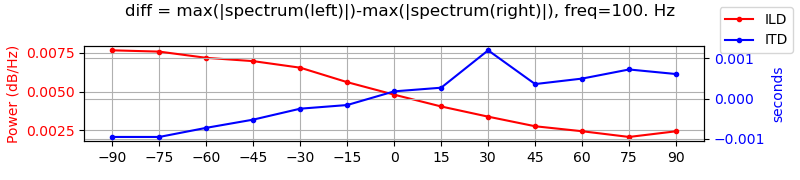
\includegraphics[width=1\linewidth]{Images/ild_itd.png}
    \caption{An example of an ITD-ILD plot from the result of an HRTF}
    \label{fig:itd-ild}
\end{figure}

\paragraph{ANF}\label{methods:anf}
Due to the differences in our peripheral processing implementations, we decided to directly evaluate the complete effect of each on the ANF spike trains. To measure the phase-locking ability of ANFs, we used vector strength (VS), a measure of phase synchrony, or how well spike timings are synchronized to a specific phase in each period. Measuring VS across the frequency spectrum is relevant to investigate how VS changes depending on the distance from the ANF characteristic frequency. Spike rate is also an important feature of ANF: since we are not modeling different rates of ANF, we expect an average spike rate of 50 to \qty{100}{\hertz} at CF.

\subsubsection{Neural processing}\label{met:neural}
As all neural layers use the same simulation, we evaluate them together. As we needed to compare results among different trials to verify whether the network could distinguish between sounds from different angles, we needed a metric for the overall evaluation. We considered two primary metrics: average spike rate for active neurons and total population spike rate. Comparisons between different populations are not very meaningful, as due to convergence, different populations have different neuron counts. In addition, the average spike rate of the population does not introduce any additional information but only scales the total population spike rate by the population size; instead, to account for different sizes, we scaled the population spikes by the number of active neurons (i.e., neurons that spiked at least once during the observation period). Although this gave additional insight, it presented an additional issue: ANFs have a high spontaneous rate, which causes them to spike across the entire frequency range. However, the filtering capability of bushy cells caused much higher rates in bushy cell layers. So, we decided that the comparatively simpler metric of the total population spike rate was used. In addition, to evaluate how different regions of each population contributed to the overall spiking pattern, we included vertical histograms for each angle, as shown in \ref{fig:rate-vs-angle}.

\begin{figure}[H]
    \centering
    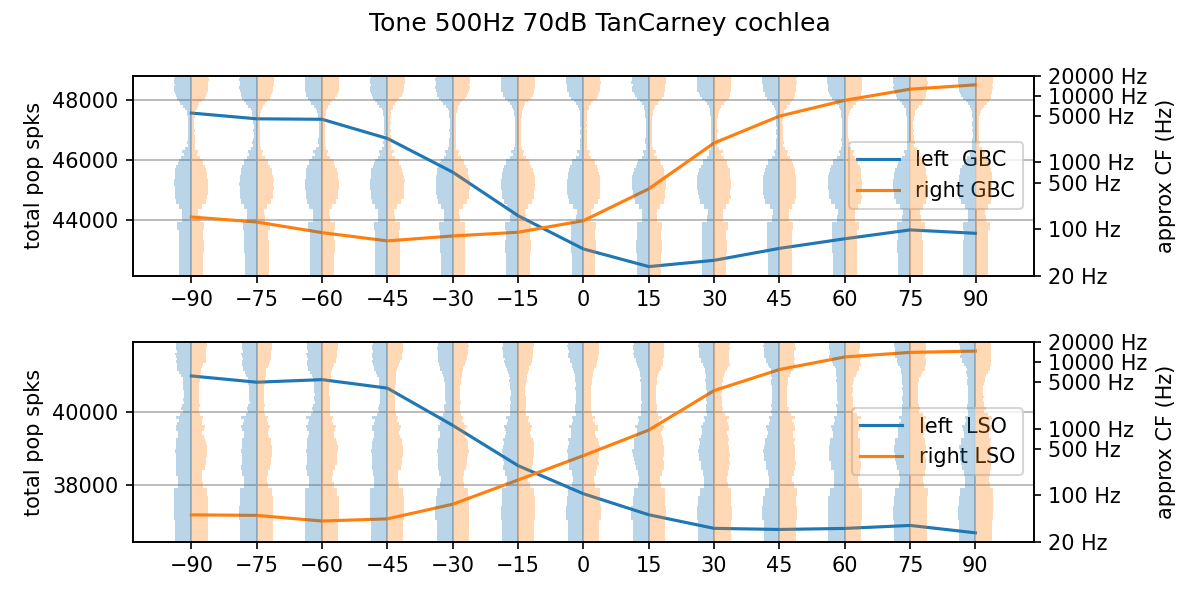
\includegraphics[width=0.5\linewidth]{Images/rate_vs_angle.png}
    \caption{An example of what a result plot looks like. On the left Y-axis, the total population spikes are shown. On the right vertical axis, we show the CF corresponding to every vertical histogram bin}
    \label{fig:rate-vs-angle}
\end{figure}

\paragraph{IC}
Our last objective is to evaluate a possible way to combine cue processing by the LSO and the MSO: drawing a simple excitatory connection from both of them (as seen in \ref{sec:ic-theory}, the IC receives inputs from ipsilateral MSO and contralateral LSO), and evaluating if the result improves compared to the LSO alone. To measure the \textit{improvement}, we fit the difference of total population spikes for each azimuthal location to a sigmoid and defined three metrics.
The general-form sigmoid function we used is the following: 
\begin{equation*}
    \frac{L}{1 + e^{-k(x - x_0)}} + b
\end{equation*}
So, our metrics will be the values that minimize non-linear least squares when applying the sigmoid to our data. The correspondence is as follows:
\begin{enumerate}
    \item \textit{$x_0$}: Closeness of center point to zero;
    \item \textit{$k$}: Steepness around zero;
    \item \textit{$L - b$}: Range, or the difference between maximum and minimum total population spike index.
\end{enumerate}
In addition, the $R^2$ value tells us how well the difference in IC spike counts can fit the sigmoid.


\subsection{Computational considerations}
As mentioned in \ref{met:nest}, the only hardware used for this work was a personal laptop. Because of this, computational efficiency and the ability to run multiple trials unattended were essential factors for the project's feasibility. This lead us to an important choice: NEST includes built-in thread parallelism but does not allow for process-level parallelism, as the \lstinline{pyNEST} library converts all calls to \lstinline{LSI} calls to the C++ kernel; inversely, brian2 does not include any support for thread parallelism, but since it is pure python it is easily process-parallelized (using \lstinline{multiprocessing} or \lstinline{joblib}). There is an additional, fundamental factor in our computation: the simulation requires a relatively large amount of RAM, ranging between \qtyrange{10}{15}{\giga\byte}. This makes process-level parallelism infeasible, as even two processes running simultaneously would cause thrashing. At the same time, only using thread-level parallelism is not the best solution: 
\begin{inlinelist}
    \item each neural simulation depends on the result of a previous, nonparallel peripheral simulation;
    \item neural simulations, when run for our average time of \qty{200}{\milli\second}, only take an average of \qty{22}{\second} to complete;
    \item peripheral simulations are recalculated on every run, even though peripheral parameters rarely change.
\end{inlinelist}

Because of this, we adapted to the limitations that our libraries imposed and formed the following workflow:
\begin{enumerate}
    \item Peripheral sections are cached. Initially, we opted for a faster, hand-built caching solution based on \lstinline{pickle}. In \ref{code:cache}, we show a simplified overview of how we initially implemented it.
    As the code grew more complicated, more parameter types were included, and more cochleas were implemented, we decided to move to a standard implementation using \lstinline{joblib.Memory} for disk-based caching. Although this resulted in a 10x slowdown in cache hits (from \qty{0.0177}{\second} to \qty{0.190}{\second}), it also included cache invalidation for changes to function code and more robust parameter serialization.
    \item The neural section uses thread-level parallelism. NEST handles parallelism quite well, and by tuning the thread count to our processors' (16), we obtained a \~8X speedup.
    \item When making significant changes to a peripheral section, or testing something that requires new generation of an \lstinline{ANFResponse}, we use a simple \lstinline{multiprocessing} based script to generate and cache all ANF responses so that the following simulation runs would only load them and not generate them. This became progressively more relevant as the complexity of our peripheral sections grew\footnote{Generating ANF spiketrains for our most bioplausible took over a minute for each side, per trial.}.
\end{enumerate}
This workflow allowed us to maximize efficiency, by parallelizing both sections of our codebase, using the most efficient version for each.

\newpage

\section{Results}
In this section, we report our findings. As for all previous sections, we maintain the sequential structure, starting with peripheral processing and progressively approaching higher-level nuclei.

\subsection{Peripheral processing}
The first approach used for objective \ref{obj: bioplaus} was modeling the processing happening outside of the ear, by using human HRTFs for realistic sound transformations. Then, we implemented one synthetic cochlea and two realistic peripheral processing pathways. The synthetic cochlea 
\begin{inlinelist}
    \item was based on Pulse Packet generators (a generator type in NEST Simulator which allows to set spike times manually); the realistic peripheral processing pathways used 
    \item a gammatone-based cochlea and
    \item the Tan Carney cochlea paired with earlier models of middle ear amplifier and IHC-ANF synapses.
\end{inlinelist}

\subsubsection{HRTF}
The effect of the head-related transfer functions was larger than we expected. Figure \ref{fig:itd-ild-diff-hrtf-freq} shows the effect of HRTF on ILD and ITD as we change the subject on which the HRTF was based (left) and the frequency of the tone (right). For what regards changing the subject, the difference was felt much more strongly in ILD curves: while some (top-left, both images bottom row) show ILD growth at -75\degree,-60\degree compared to -90\degree before decreasing, others (top-right, center left) immediately decrease; at the other end, most responses show a non-monotonic decrease, with the final +90\degree varying in magnitude; there is a strong asymmetry shown in most responses, with the response never crossing the x-axis in correspondence with zero difference, as in Figure~\ref{fig:hrtf-anf}. 
\begin{figure}[H]
    \centering
    % 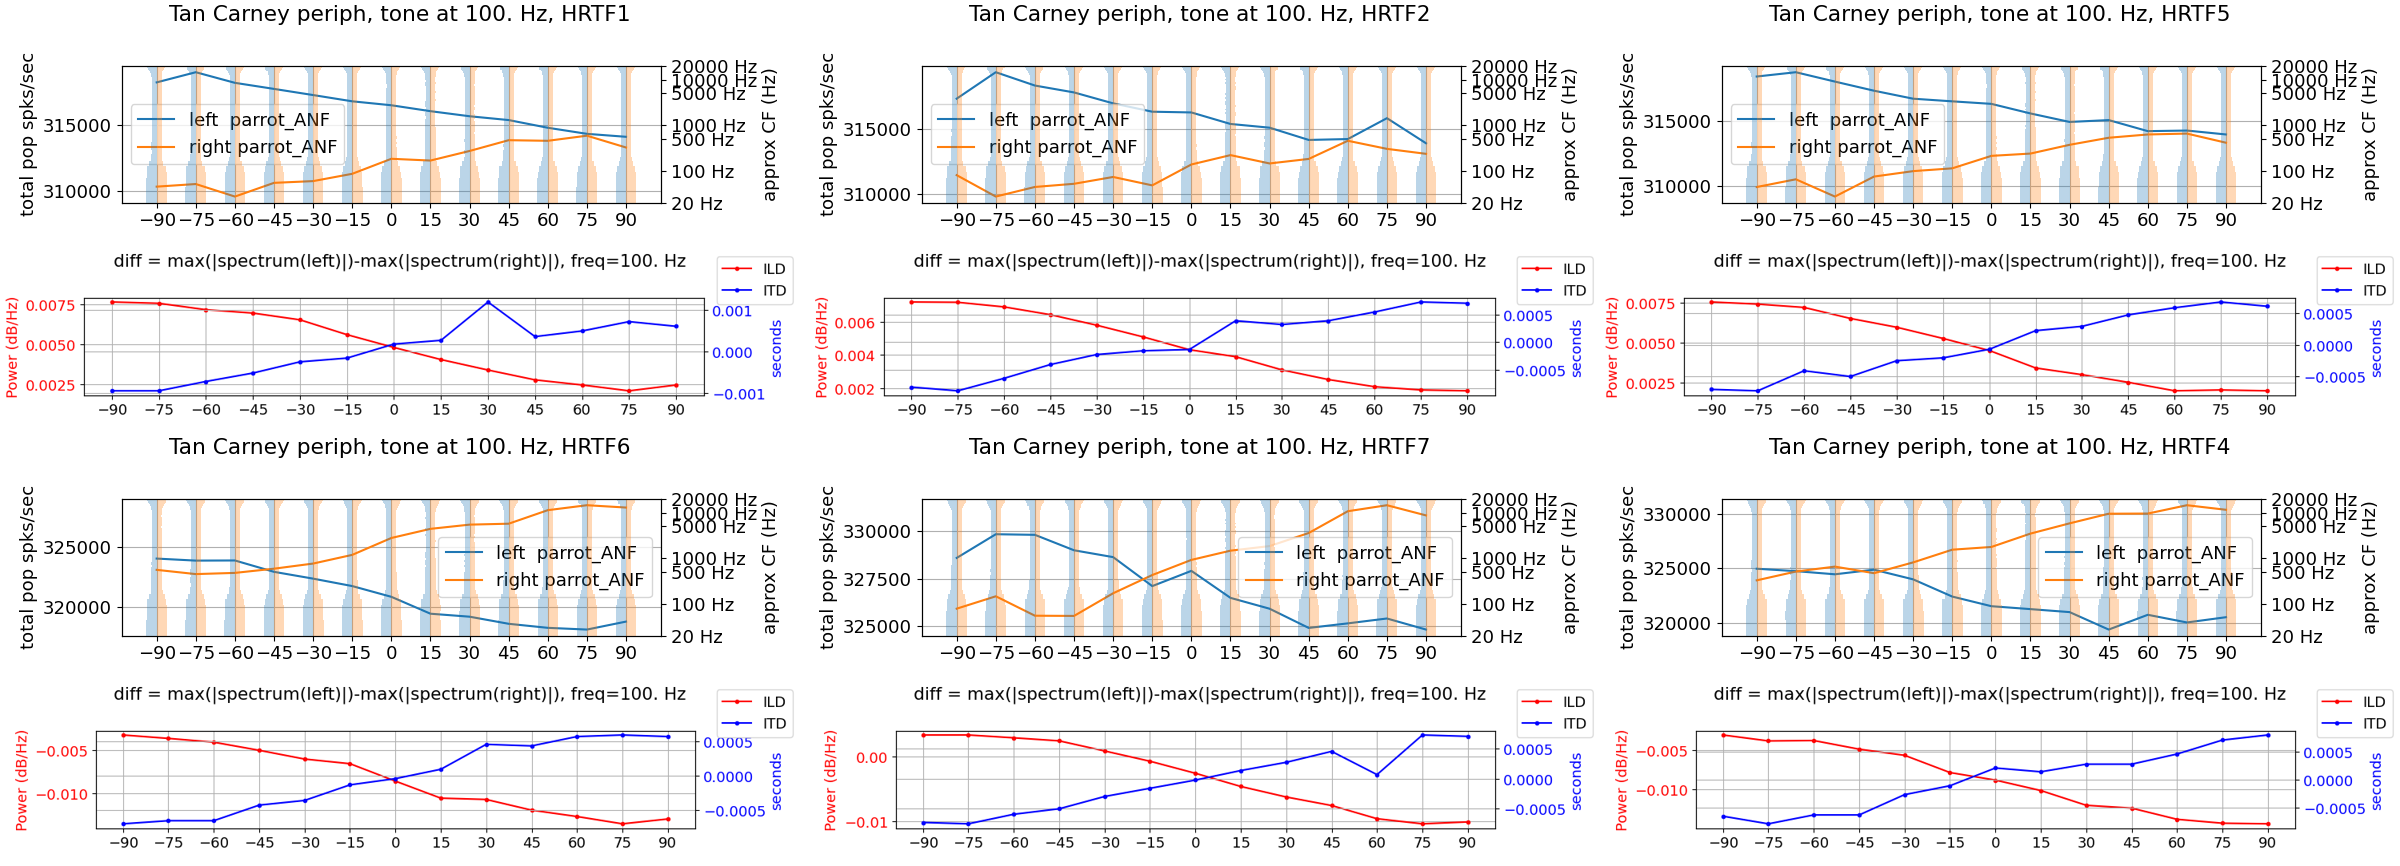
\includegraphics[width=\linewidth]{Images/ANFfordiffHRTF.png}
    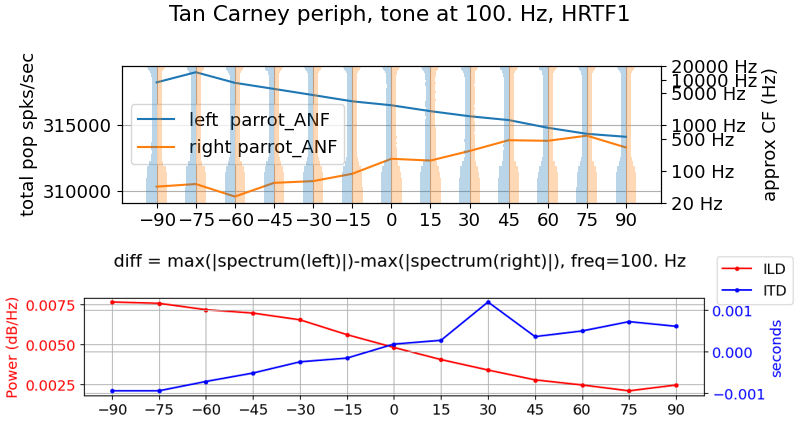
\includegraphics[width=0.45\linewidth]{Images/hrtf1.png}
    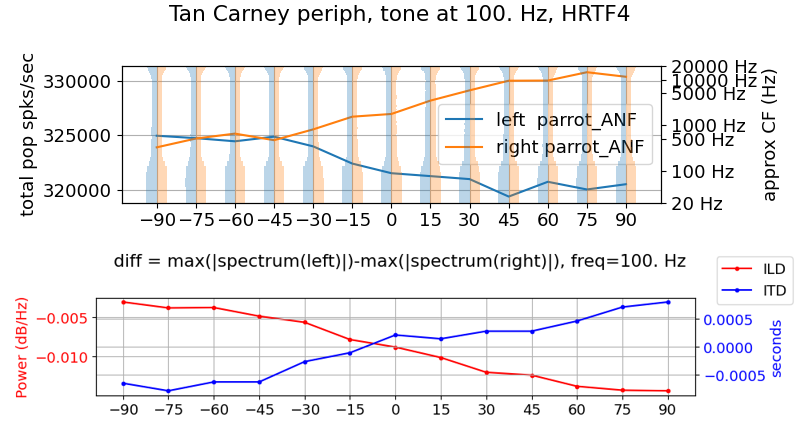
\includegraphics[width=0.45\linewidth]{Images/hrtf4.png}
    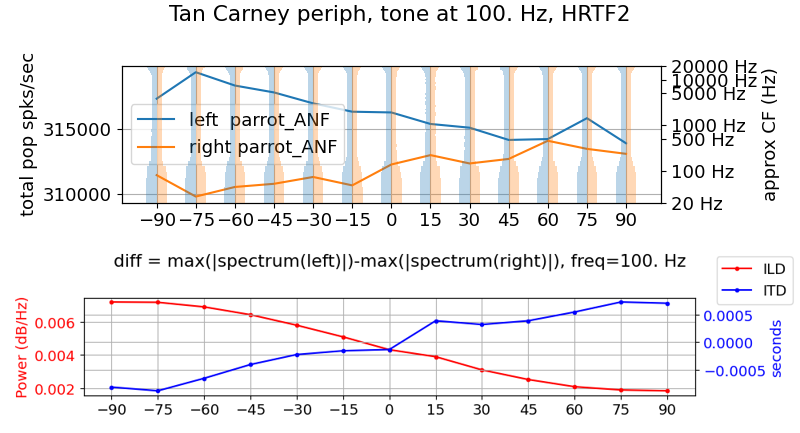
\includegraphics[width=0.45\linewidth]{Images/hrtf2.png}
    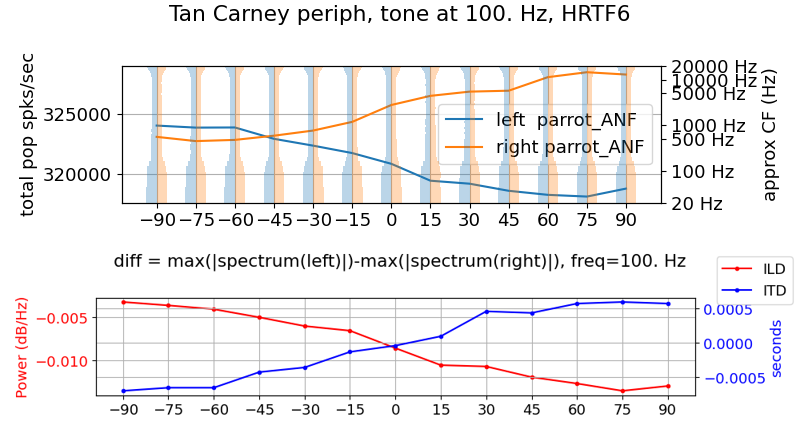
\includegraphics[width=0.45\linewidth]{Images/hrtf6.png}
    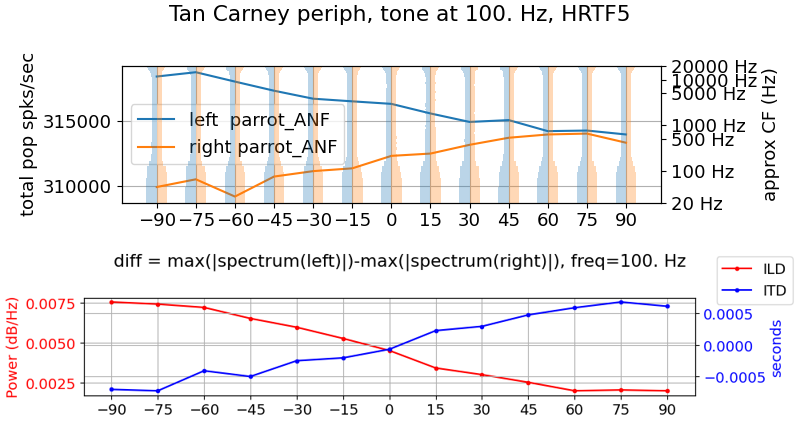
\includegraphics[width=0.45\linewidth]{Images/hrtf5.png}
    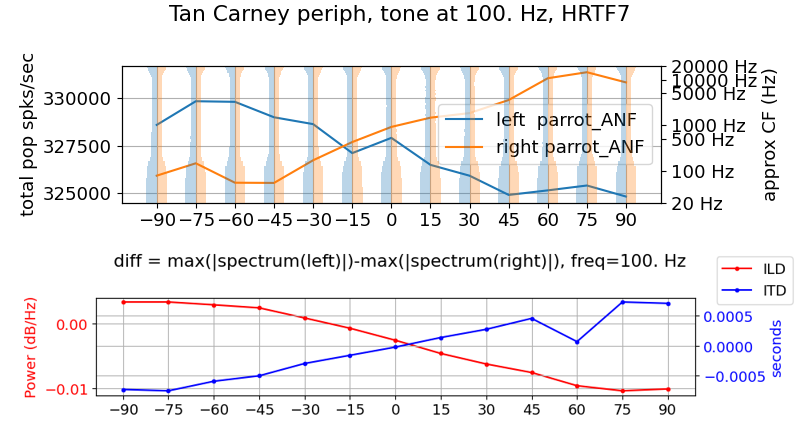
\includegraphics[width=0.45\linewidth]{Images/hrtf7.png}
    \caption{ANF responses for different HRTFs. In the left column, HRTFs where the left ear always receives a higher level than the right ear, and in the right column, HRTFs where the right ear mostly receives a higher level than the left ear.}
    \label{fig:hrtf-anf}
\end{figure}


The results in responses to different frequencies are as expected, as ILD size increases as frequency increases, while ITD remains constant. ITDs show some noise in their responses.

\begin{figure}[H]
    \centering
    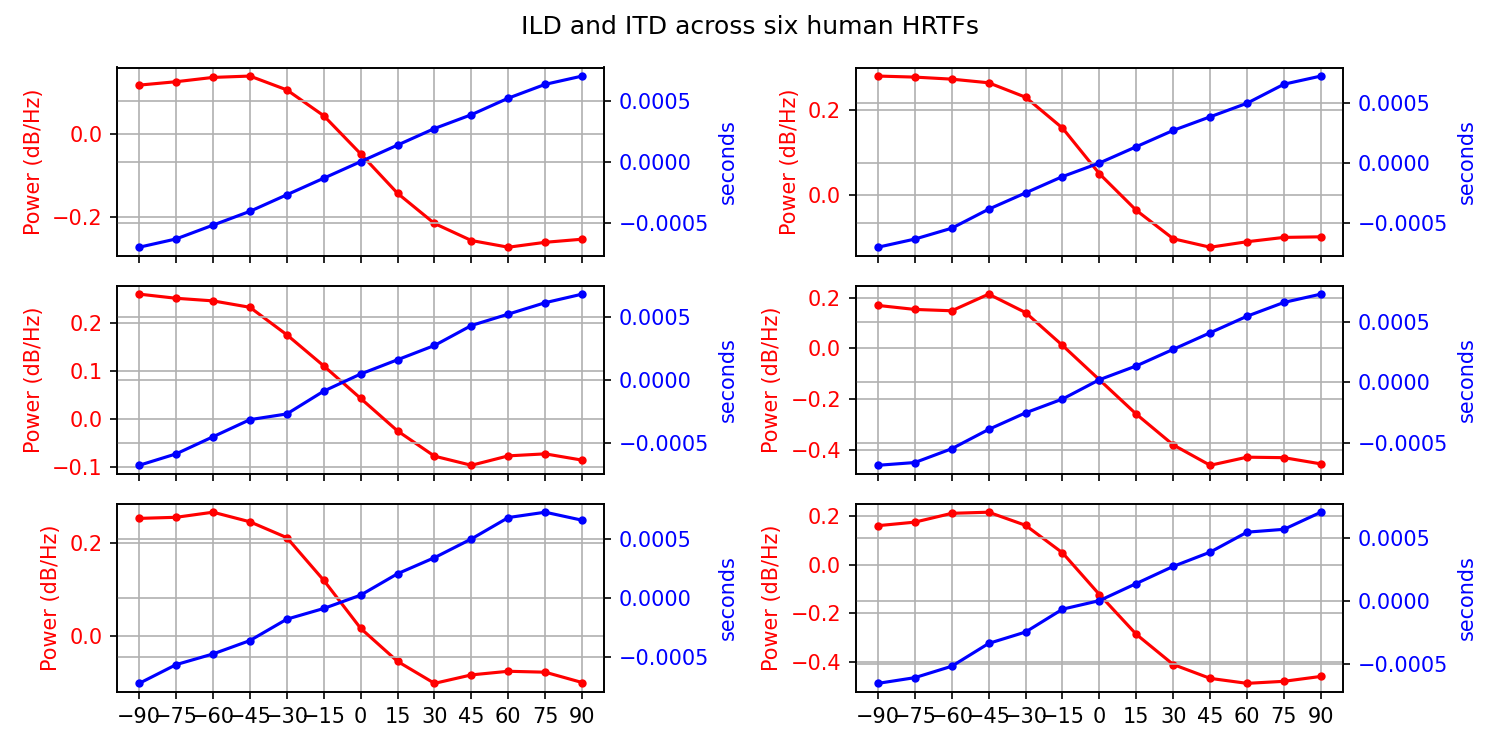
\includegraphics[width=0.48\linewidth]{Images/itd_ild_diff_hrtf.png}
    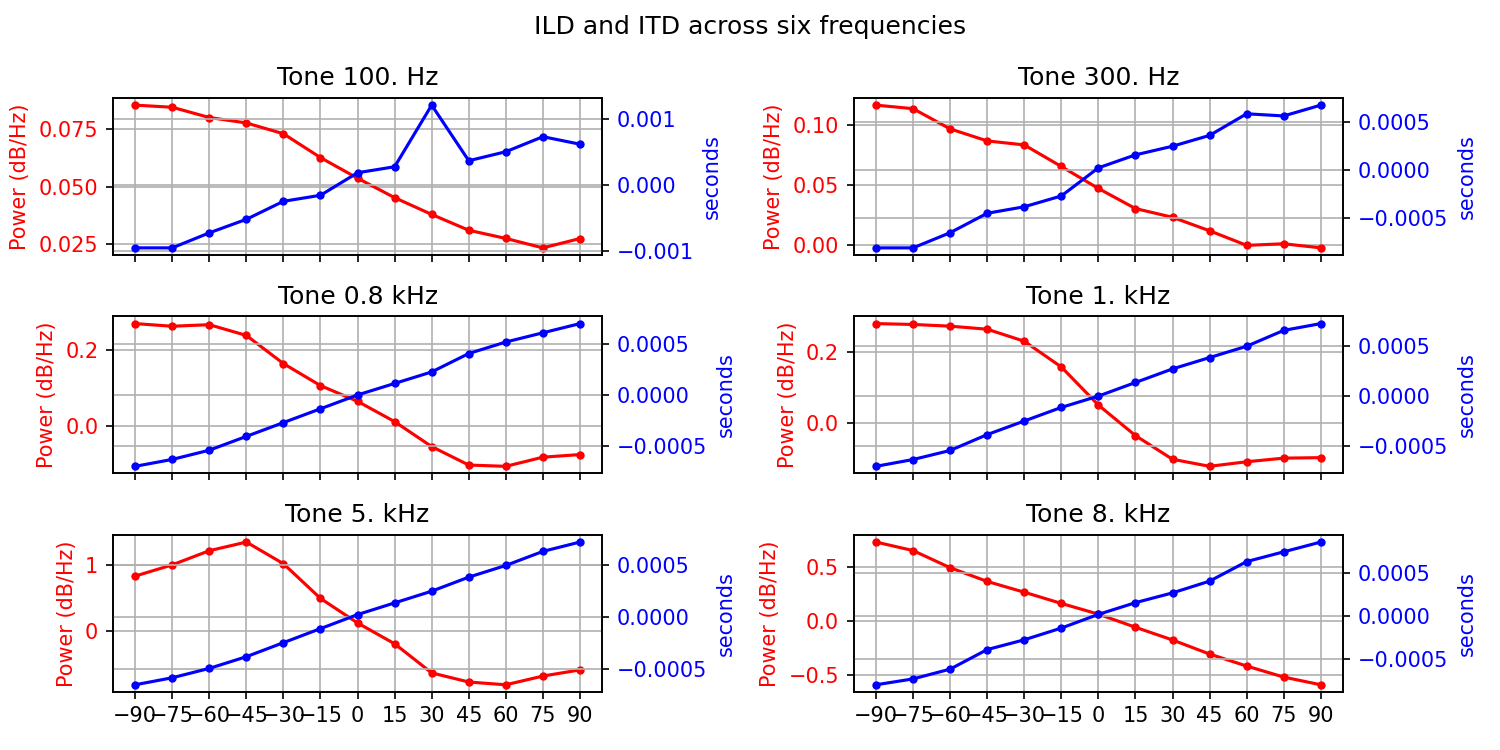
\includegraphics[width=0.48\linewidth]{Images/itd_ild_diff_freq.png}
    \caption{The effects on measured ITD and ILD for varying human HRTF (left) and varying frequencies (right). The six human HRTFs were tested using a \qty{1}{\kilo\hertz} tone.}
    \label{fig:itd-ild-diff-hrtf-freq}
\end{figure}

\subsubsection{Non neural processing}
As mentioned in \ref{methods:anf}, we evaluate peripheral processing pathways based on the ANF response, focusing on vector strength (VS). Our results are collected in \ref{fig:vectorstrength}. 
\begin{figure}[H]
    \centering
    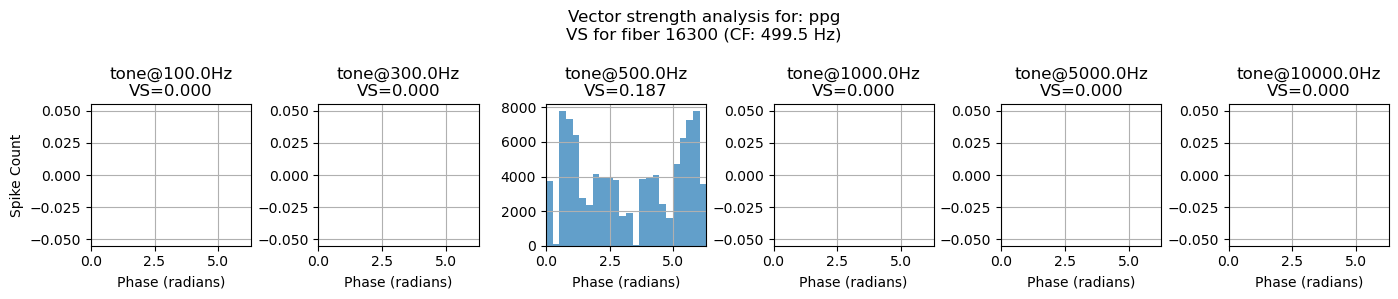
\includegraphics[width=1\linewidth]{Images/VSppg.png}
    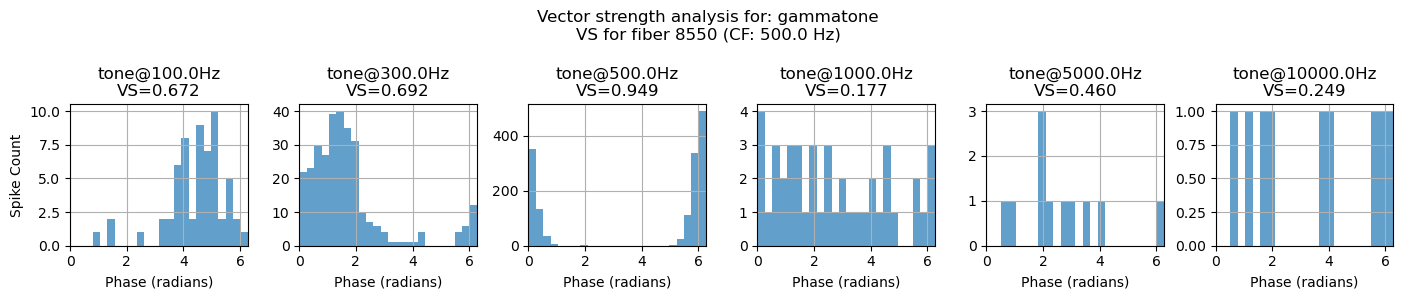
\includegraphics[width=1\linewidth]{Images/VSgamm.png}
    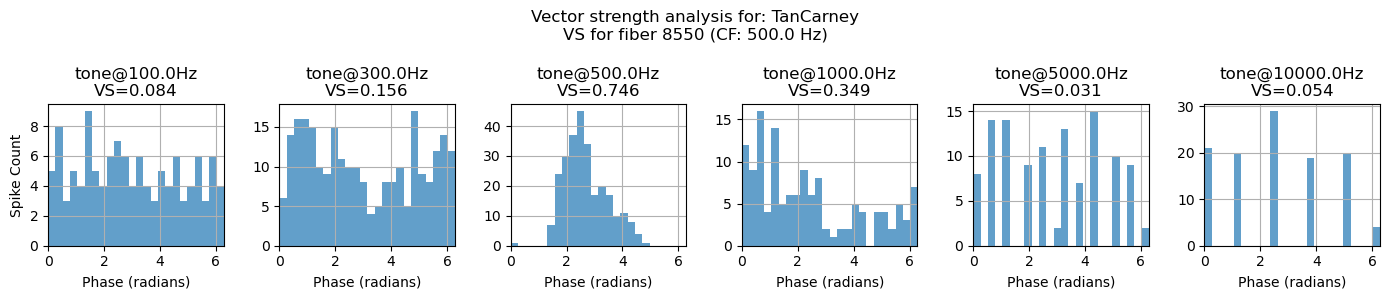
\includegraphics[width=1\linewidth]{Images/VStancarney.png}
    \caption{Vector strength plots for the three peripheral sections}
    \label{fig:vectorstrength}
\end{figure}
In the figure we plot an analysis of the spiking behavior of a single auditory nerve fiber, one of the ten connected to the IHC, with the characteristic frequency listed above. The inputs were three-second tones, with the frequencies listed above each column of plots. The results show that using more biologically plausible peripheral processing results in higher-quality ANF spike trains. We highlight the main findings here:
\begin{inlinelist}
    \item pulse packet generators were extremely faithful in tonotopic activation, as the only spiking ANFs are those in the immediate surrounding (a range of 2100 ANFs), which is in disagreement with the more bioplausible options
    \item the phase locking exhibited by the synthetic processing was very limited
    \item\label{vs:gamm} the gammatone-based processing shows very accurate phase locking for ANFs whose CFs were close to the input frequency, with a slow falloff in ANFs further away from CF
    \item total number of spikes with gammatone-based processing is much higher than the most bioplausible version at CF, but falls off very quickly, possibly masking a lower phase locking than shown
    \item the most bioplausible processing shows comparatively low spiking rates, which fall off slowly in ANFs with different CFs, and 
    \item\label{vs:tclowfreq} lower CF ANFs are still active even if the CF is further away.
\end{inlinelist}
These findings show the superiority of a realistic, bioplausible processing: higher vector strength (hence phase locking), more realistic spike counts with a less drastic falloff and some spontaneous rates, and more realistic falloff of ANF activation as CF changes.

\subsection{Neural processing}
Once ANF spiketrains were generated (and cached), they became the input to our neural simulation. As mentioned in \ref{met:neural}, both total population spike rate and active neuron spike rate are shown as population spiking metrics, depending on what the focus is. In this section, we will analyze how information flowed to each population.

\subsubsection{Intermediate populations}
The role of bushy cells is to filter the ANF input. In \ref{fig:res-singlespike-bushy}, we show the raster plot of spiking behavior from a range of neurons surrounding the cells with CF closest to the input tone (here, \qty{100}{\hertz}). The corresponding index to CF in ANFs was determined from the rule that every IHC has 10 ANFs attached to it, while the other was calculated from the convergence rules. The striped patterns shown are a feature of the tonotopic organization of the cochlea as CFs grow exponentially.

\begin{figure}[H]
    \centering
    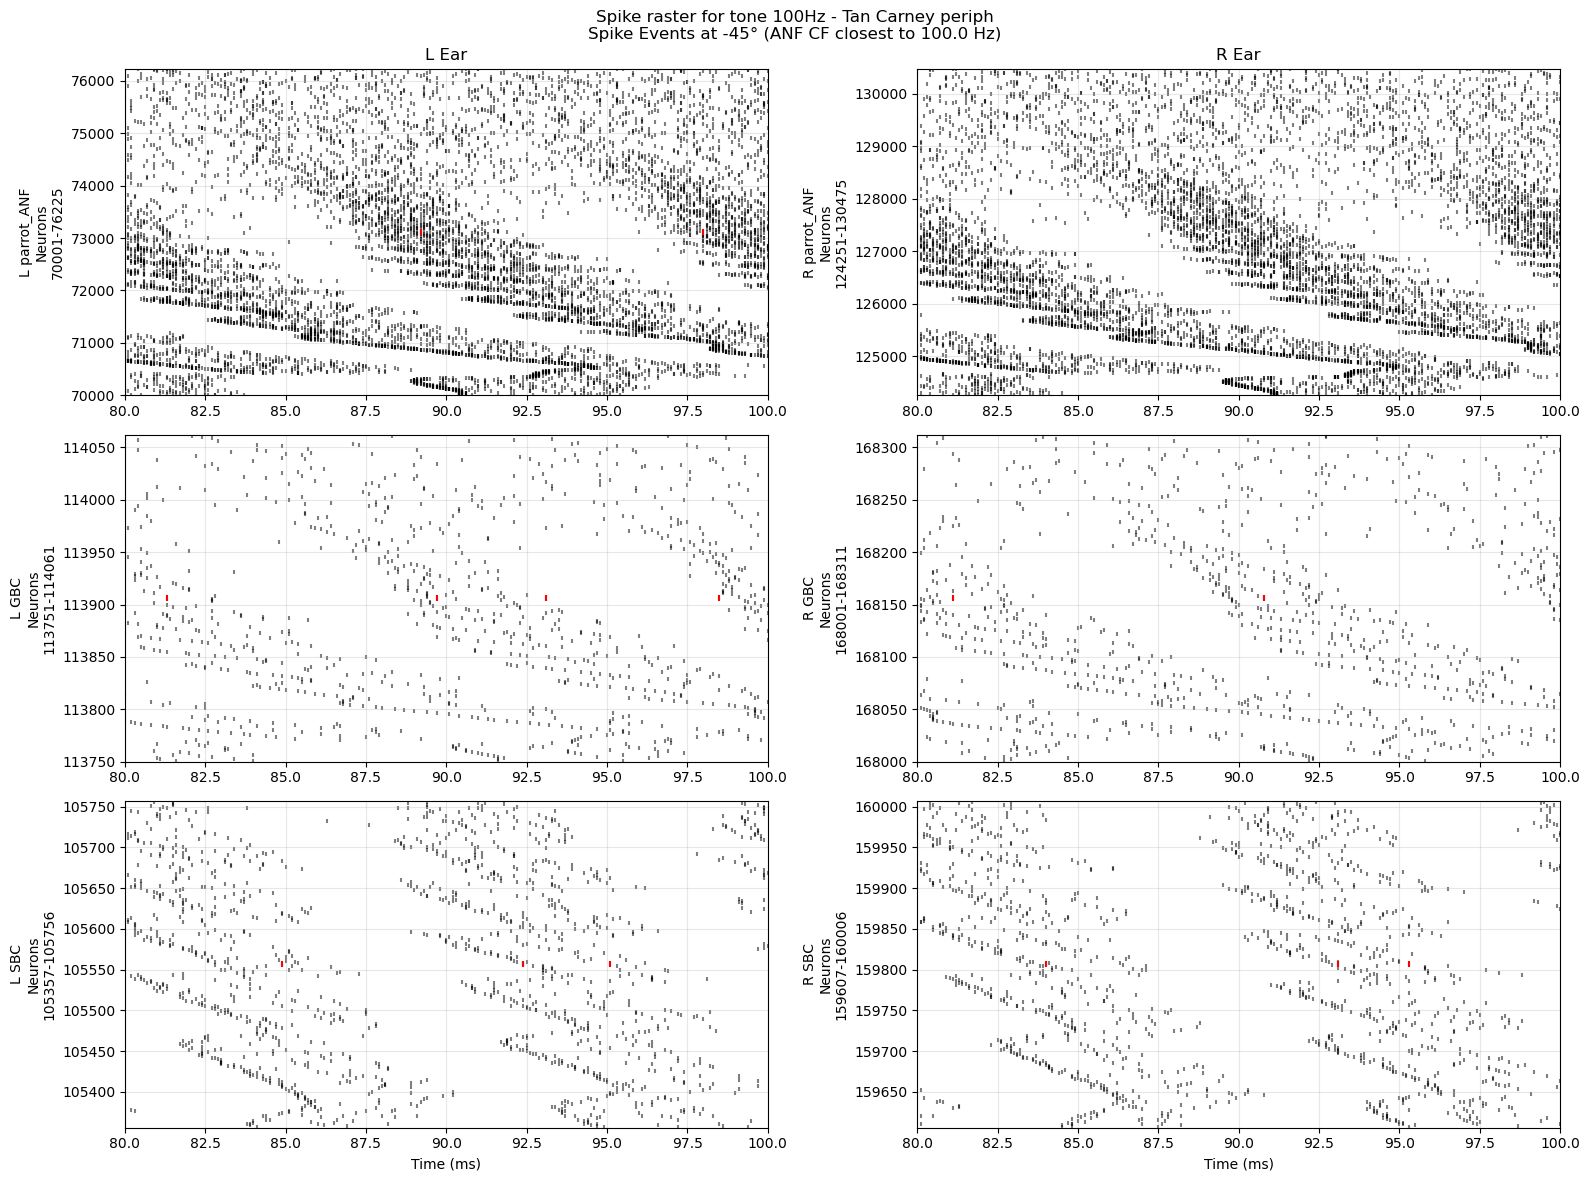
\includegraphics[width=0.75\linewidth]{Images/raster_bushy.png}
    \caption{Raster plots of neurons surrounding CF in ANFs and bushy cell populations. Due to population size differences, ANF plots show spikes from a range much larger than bushy layers.}
    \label{fig:res-singlespike-bushy}
\end{figure}

Following populations, cells in the LNTB and MNTB do not show any change in spiking rates from their input, the GBCs. This is consistent with the literature, as GBCs form strong and stable synapses, and the role of LNTB and MNTB is to relay their signals and faithfully transform them into inhibitory contributions.

\begin{figure}[H]
    \centering
    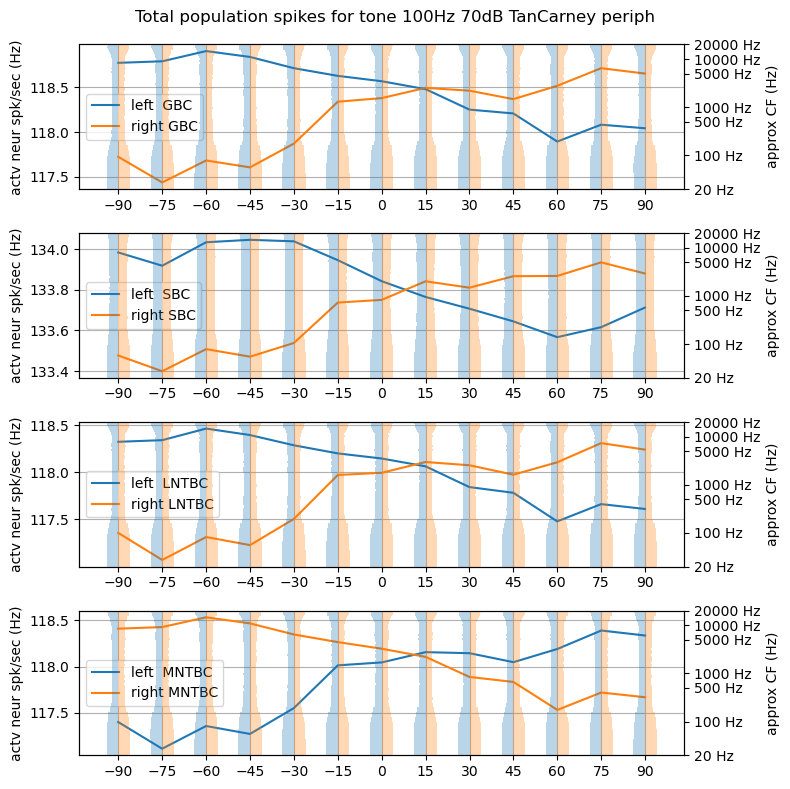
\includegraphics[width=0.7\linewidth]{Images/pop_spike_mntb_lntb.png}
    \caption{Population spiking rates for 100Hz tone}
    \label{fig:res-lntb-mntb-pop-rate}
\end{figure}

\subsubsection{Higher centers}
We now move to analyzing the spiking behaviors of nuclei in the SOC, the LSO, and the MSO. 

\paragraph{LSO}
In our testing, the LSO was remarkably stable. Even at low frequencies, where the sizes of ILD are considered minute, the shape of the LSO was unmistakable and very resistant to perturbations. The LSO remained consistent when membrane time constants and weights were changed. It was also generated equally well by both realistic cochleas, as shown in \ref{fig:res-lso}. The difference between spike volumes of the two sides increased, as is to be expected with the rising ILD, as frequency increased. When using the gammatone-based peripheral section, the LSO failed above \qty{10}{\kilo\hertz}.

\begin{figure}[H]
    \centering
    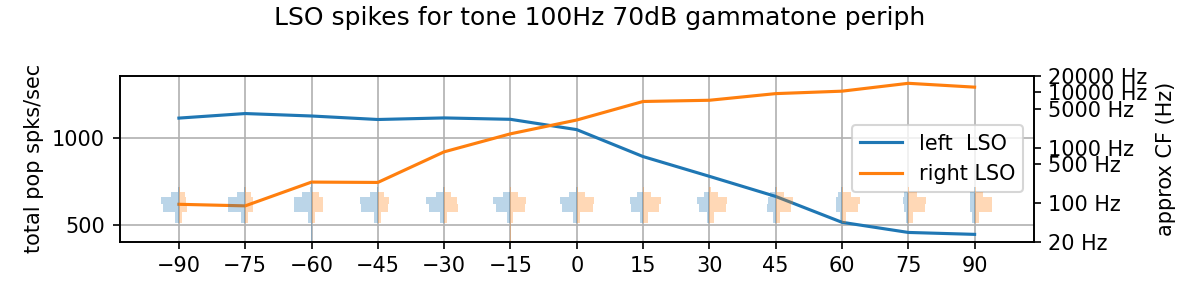
\includegraphics[width=0.4\linewidth]{Images/lso100.png}
    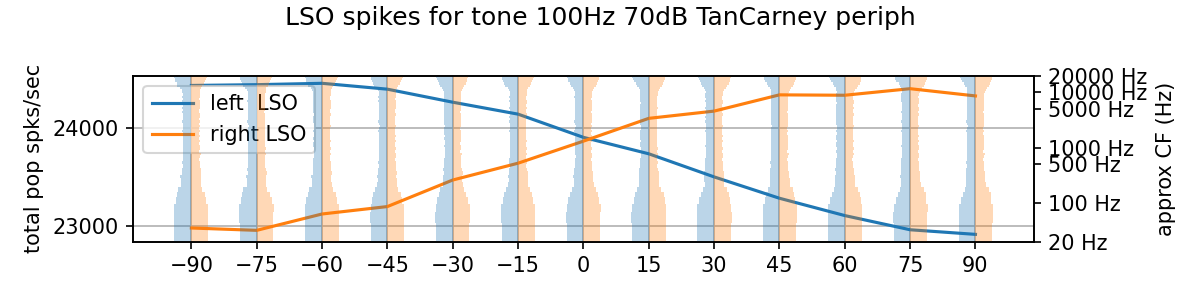
\includegraphics[width=0.4\linewidth]{Images/lso100tc.png}
    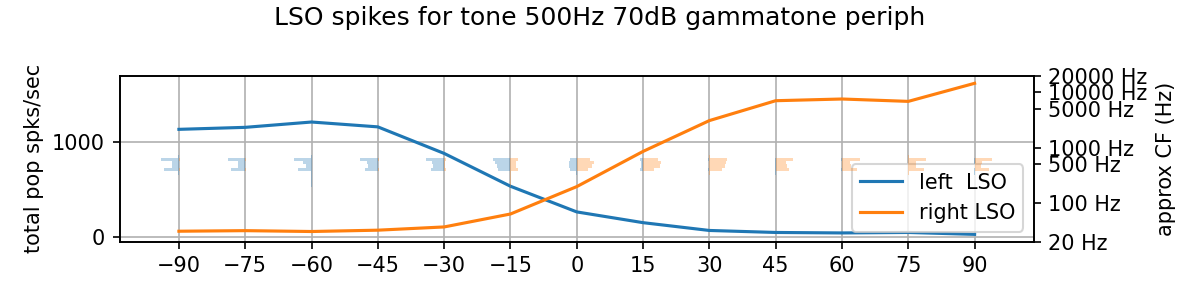
\includegraphics[width=0.4\linewidth]{Images/lso500.png}
    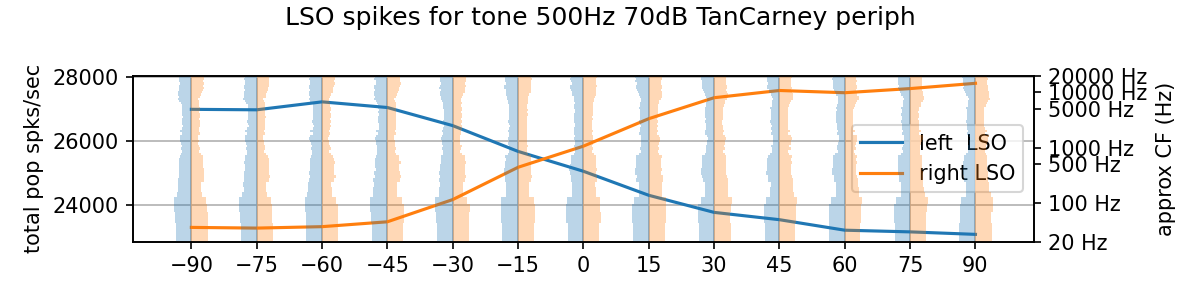
\includegraphics[width=0.4\linewidth]{Images/lso500tc.png}
    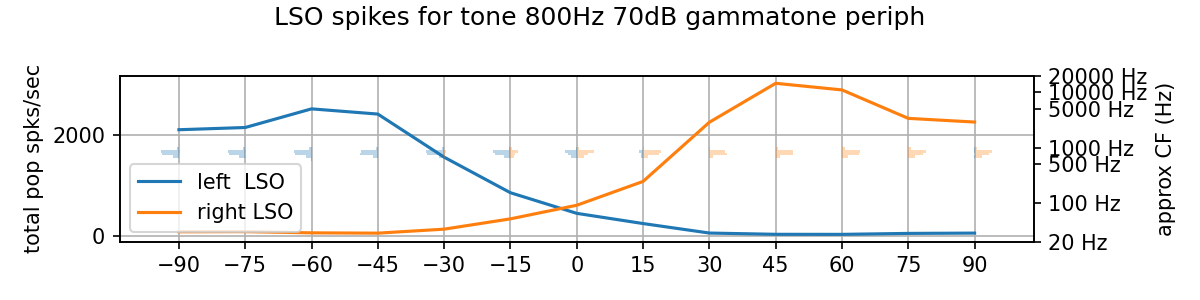
\includegraphics[width=0.4\linewidth]{Images/lso800.png}
    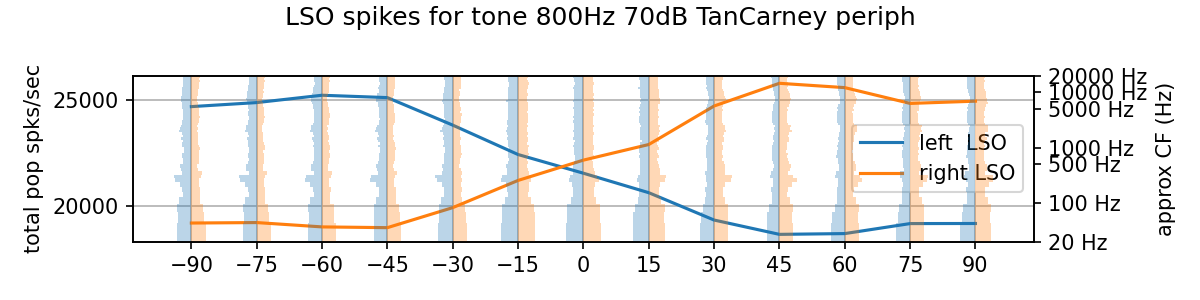
\includegraphics[width=0.4\linewidth]{Images/lso800tc.png}
    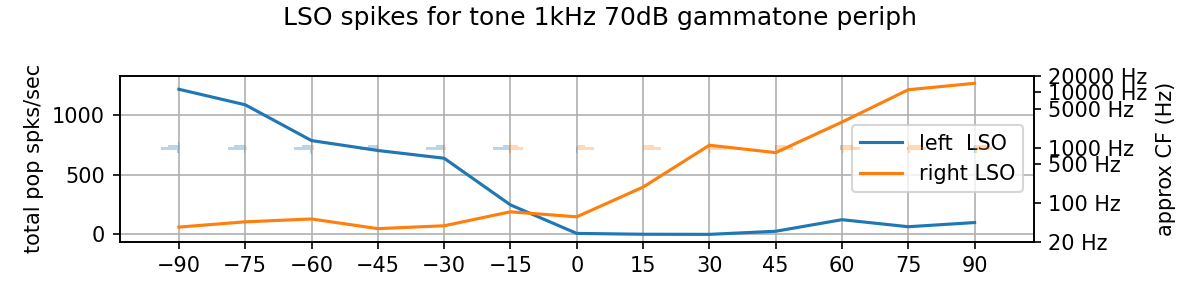
\includegraphics[width=0.4\linewidth]{Images/1khz.png}
    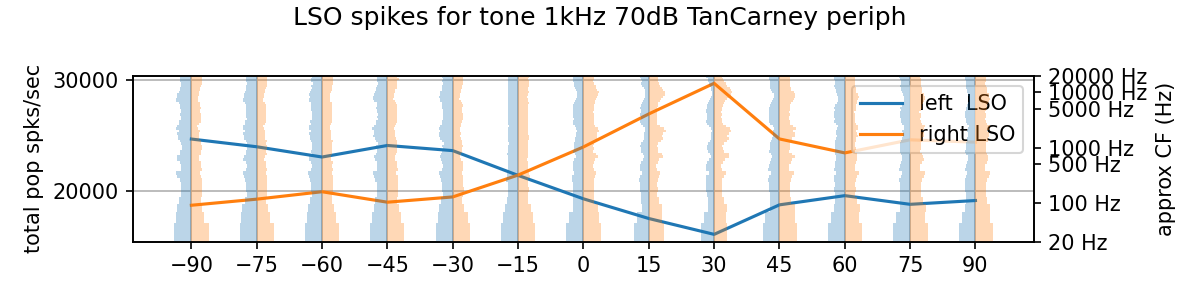
\includegraphics[width=0.4\linewidth]{Images/lso1000tc.png}
    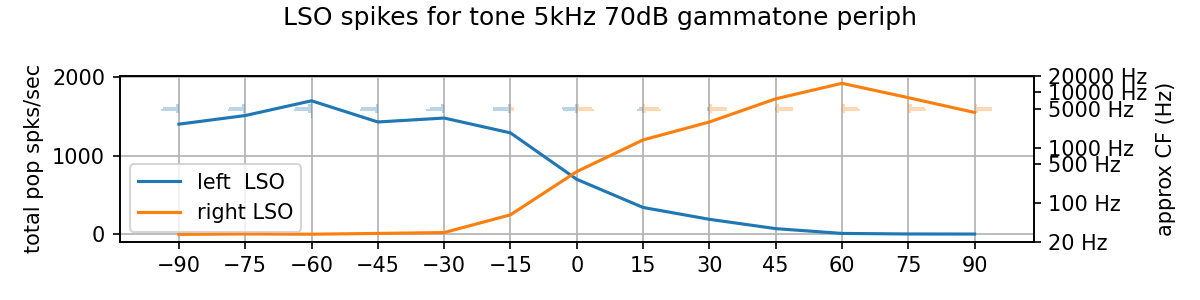
\includegraphics[width=0.4\linewidth]{Images/lso5khz.png}
    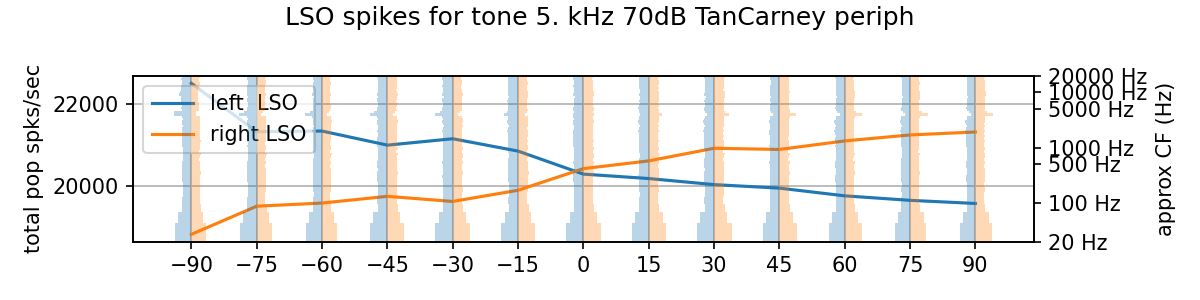
\includegraphics[width=0.4\linewidth]{Images/lso5000tc.png}
    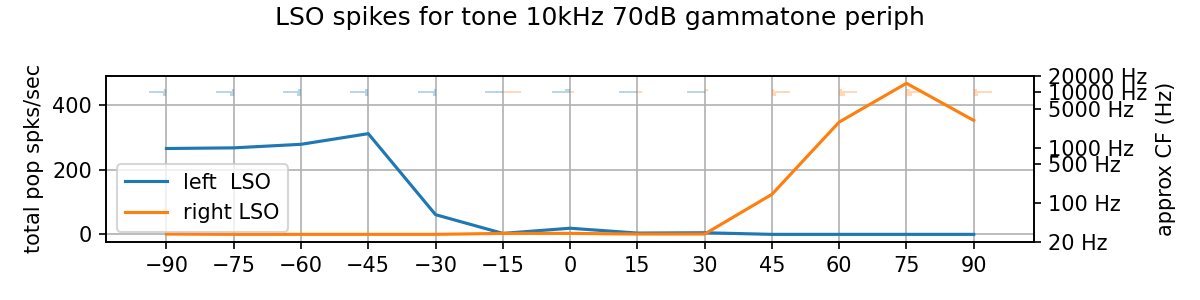
\includegraphics[width=0.4\linewidth]{Images/lso10khz.png}
    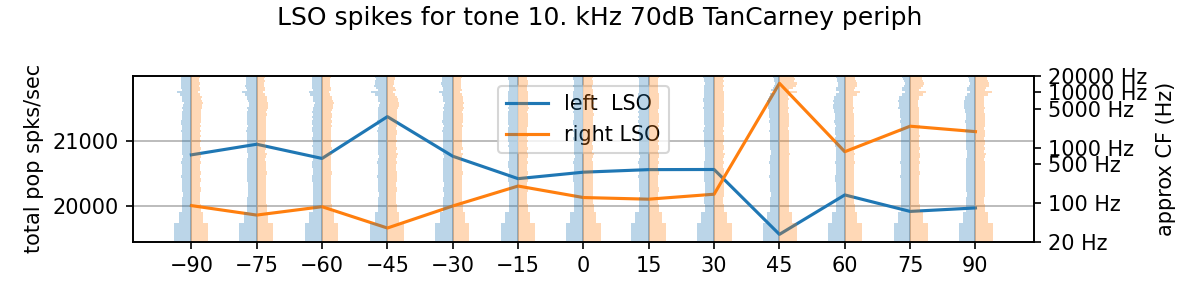
\includegraphics[width=0.4\linewidth]{Images/lso10000tc.png}
    \caption{Population spike rates for the LSO with growing frequencies, for gammatone-based (left) and Tan Carney (right) processing.}
    \label{fig:res-lso}
\end{figure}

\paragraph{MSO}
As with the LSO, the largest difference between the two peripheral processing is the size of involved frequency ranges: while the gammatone-based processing only activates a narrow portion of ANFs (and hence the rest of the network), the more bioplausible inputs generate a broader activation. At the same time, MSO cells with high CF activate much less in proportion, possibly due to the slower decay time of inhibition, which, at high frequencies, stops cells almost completely. Decay with rising frequency is not the same between the two input sources: while the gammatone-based falls off quickly, losing differentiating abilities at \qty{800}{\hertz}, the Tan Carney-based continues to maintain efficacy (except for at \qty{1}{\kilo\hertz}) to \qty{10}{\kilo\hertz}.
\begin{figure}[H]
    \centering
    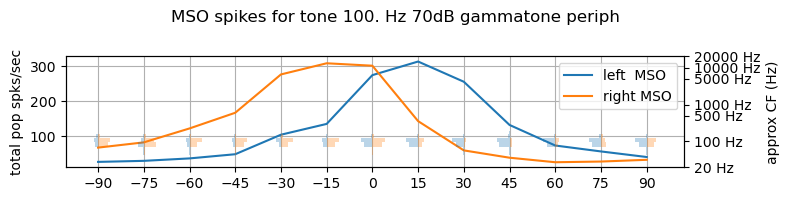
\includegraphics[width=0.48\linewidth]{Images/gamm100.png}
    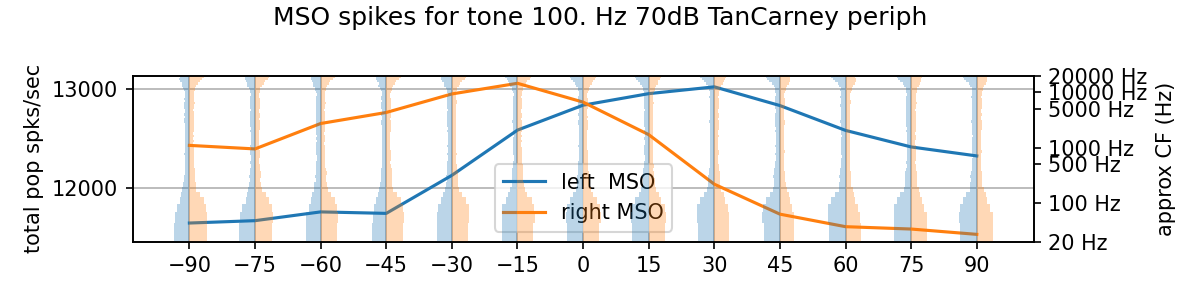
\includegraphics[width=0.48\linewidth]{Images/mtc100.png}
    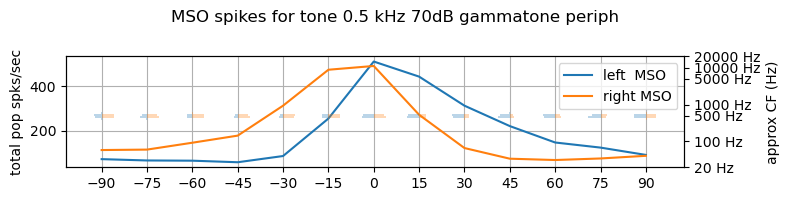
\includegraphics[width=0.48\linewidth]{Images/gamm500.png}
    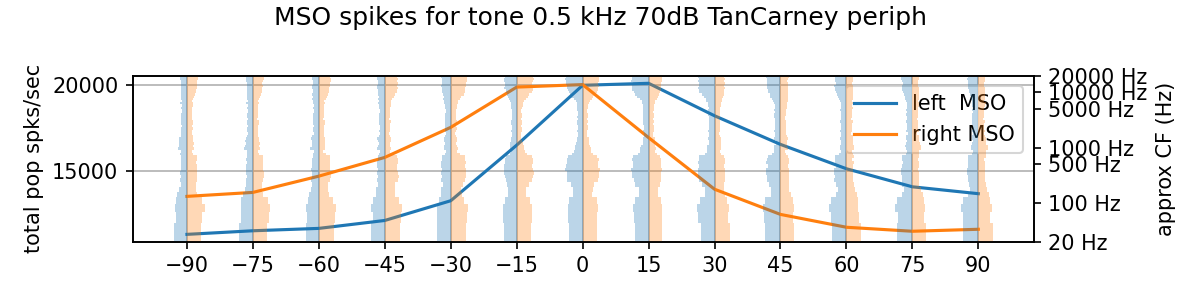
\includegraphics[width=0.48\linewidth]{Images/mtc500.png}
    \includegraphics[width=0.48\linewidth]{Images/gamm800.png}
    \includegraphics[width=0.48\linewidth]{Images/mtc800.png}
    \includegraphics[width=0.48\linewidth]{Images/gamm1000.png}
    \includegraphics[width=0.48\linewidth]{Images/mtc1000.png}
    \includegraphics[width=0.48\linewidth]{Images/gamm5000.png}
    \includegraphics[width=0.48\linewidth]{Images/mtc5000.png}
    \includegraphics[width=0.48\linewidth]{Images/gamm10000.png}
    \includegraphics[width=0.48\linewidth]{Images/mtc10000.png}
    \caption{Population spike rates for the MSO with growing frequencies, for gammatone-based (left) and Tan Carney (right) processing.}
    \label{fig:res-mso}
\end{figure}


\subsection{IC and integrating cues}
Finally, we consider whether the integration of cues from MSO and LSO proved beneficial to the IC. To determine the impact of the MSO on the IC curves, we focus on the most bioplausible version of our peripheral processing. In \ref{fig:lso-icc-fit-sigmoid}, we plot the difference of total population spikes between the right and left LSO (top) and IC (bottom). All differences are collected in table \ref{tab:lso-icc-fit}. The results are not particularly striking: while the steepness around the center point improved, this came at a cost for range, which decreased in the IC compared to the LSO. Overall, the zero crossing accuracy was the most significant improvement, which at low frequencies was increased significantly. At the same time, due to database constraints, our data points are 15 degrees apart, and even the largest improvement in zero crossing was only by around 3 degrees, which is not a significant improvement.


\begin{figure}[H]
    \centering
    \includegraphics[width=1\linewidth]{Images/LSOfit.png}
    \includegraphics[width=1\linewidth]{Images/ICCfit.png}
    \caption{Comparison of sigmoid fit for all frequencies. Top: LSO. Bottom: IC. Because the contralateral LSO connects to IC, its slope is in the opposite direction.}
    \label{fig:lso-icc-fit-sigmoid}
\end{figure}

\begin{table}[htbp]
\centering
\caption{Analysis of improvement of ICC over LSO}
\label{tab:lso-icc-fit}
\begin{tabular}{r|rrr|r}
\hline
\multicolumn{5}{c}{\textbf{STEEPNESS}} \\
\hline
Frequency & LSO & ICC & Diff & Improvement \\
\hline
100 & 0.034 & 0.040 & 0.005 & 15.5\% \\
500 & 0.057 & 0.067 & 0.010 & 16.8\% \\
800 & 0.043 & 0.051 & 0.008 & 18.7\% \\
1000 & 0.094 & 0.104 & 0.010 & 10.2\% \\
5000 & 0.033 & 0.041 & 0.008 & 24.4\% \\
10000 & 0.037 & 0.045 & 0.009 & 23.2\% \\
\hline
Average & & & & 18.1\% \\
\hline
\multicolumn{5}{c}{\textbf{R\_SQUARED}} \\
\hline
Frequency & LSO & ICC & Diff & Improvement \\
\hline
100 & 0.997 & 0.997 & 0.000 & 0.0\% \\
500 & 0.998 & 0.998 & -0.000 & -0.0\% \\
800 & 0.994 & 0.992 & -0.002 & -0.2\% \\
1000 & 0.995 & 0.991 & -0.004 & -0.4\% \\
5000 & 0.985 & 0.986 & 0.001 & 0.1\% \\
10000 & 0.942 & 0.909 & -0.033 & -3.5\% \\
\hline
Average & & & & -0.7\% \\
\hline
\multicolumn{5}{c}{\textbf{RANGE}} \\
\hline
Frequency & LSO & ICC & Diff & Improvement \\
\hline
100 & 3266.574 & 3321.874 & 55.301 & 1.7\% \\
500 & 2826.344 & 2691.311 & -135.032 & -4.8\% \\
800 & 3296.494 & 2882.988 & -413.506 & -12.5\% \\
1000 & 2747.825 & 2505.705 & -242.119 & -8.8\% \\
5000 & 1807.770 & 1185.965 & -621.805 & -34.4\% \\
10000 & 2214.870 & 1455.782 & -759.088 & -34.3\% \\
\hline
Average & & & & -15.5\% \\
\hline
\multicolumn{5}{c}{\textbf{ZERO-CROSSING ACCURACY}} \\
\hline
Frequency & LSO & ICC & Diff & Improvement \\
\hline
100 & 10.316 & 7.556 & 2.759 & 26.7\% \\
500 & 12.788 & 10.226 & 2.562 & 20.0\% \\
800 & 9.356 & 8.534 & 0.822 & 8.8\% \\
1000 & 4.197 & 3.662 & 0.535 & 12.7\% \\
5000 & 4.942 & 3.942 & 1.001 & 20.2\% \\
10000 & 5.660 & 4.202 & 1.458 & 25.8\% \\
\hline
Average & & & & 19.1\% \\
\hline
\end{tabular}
\end{table}

\newpage
\section{Discussion}
Our results show significant improvements on multiple fronts but also limits to our model. We consider some of them here.

\subsection{Peripheral processing}
Overall, we found significant advantages in implementing and testing bioplausible peripheral processing sections. The most impactful feature covered the unavailability of data: most bioplausible models are tested against existing recordings and features, but the original data is limited and difficult to obtain. Because of this, our more advanced processing pipeline was able to inform things like the multiplicative scalar for the gammatone-based peripheral processing. On the other hand, the Tan-Carney-based model for ANFs, because of its bioplausibility, did not produce ANFs strictly sectioned to a frequency range, which affected our parameter search: for example, when using high enough weights for inhibition, the MSO stops considering high-frequency data, and the only fibers that remain active are the ones with low CF. On the other hand, our least bioplausible ANF model did not produce useful results, as its spikes were so closely aligned that the parameter values needed to allow their processing were entirely different from both other models.

Our bioplausible models imposed two limitations on us: the 15\degree increments in possible azimuthal positions and the adaptation shown by the bioplausible IHC-ANF synapse due to vesicle availability. The first could be tackled by including a more modern approach to HRTF filtering, such as the python library \lstinline{sofar}. In contrast, the second one, also true in biological experiments, can be solved by repeating the stimulus multiple times in a brief window.

\subsection{Neural pathway}
The intermediate populations of our neural processing resulted in modestly bioplausible results: while bushy cells were able to phase lock to low-frequency stimuli, our modeling did not include significant differences between spherical and globular bushy cells beyond their convergence values, and no individual differences among the population. Still, they accomplished their filtering task and were able to bring reliable, phase-locked PSPs to the upper nuclei.

\subsection{MSO}
In our modeling of the MSO, we confirm the findings of Myoga and the limitation of this approach: the maximal shift we could confirm was $\pm200ms$, roughly equivalent to $\pm30\degree$ with human head size. This would not be very compatible with a two-channel approach, as it would only be able to determine sound location in a very narrow band of locations in front of the subject; this is not compatible with behavioral evidence. It also does not offer sufficient range to provide a map of ITDs. At the same time, while experimenting with this approach, we learned that it may be possible to use the relative strength of the two inhibition sources to drive the angle of maximal response. A preliminary finding is shown in \ref{fig:myoga-vary-weight}.
\begin{figure}[H]
    \centering
    \includegraphics[width=0.5\linewidth]{Images/myoga_change_weights.png}
    \caption{Colormap showing which angle (hence ITD) makes MSO reach maximum voltage when varying strength of inhibition sources. Both excitation sources are kept at weight 6}
    \label{fig:myoga-vary-weight}
\end{figure}

\subsection{LSO}
As mentioned, the LSO had remarkably stable outputs, which reliably showed differences (modest at low frequencies, larger at high frequencies) between sides. The modest difference at low frequencies is also due to a limited sensibility to ITD from the LSO: in Figure \ref{fig:lso-itdonly} we show the spike behavior of the LSO with an input tone filtered through an artificial HRTF which only includes ITD information and no spectral (hence no ILD) differences. A slight sensitivity to ITD by LSO is also documented in literature \cite{yinNeuralMechanismsBinaural2019}.
\begin{figure}[H]
    \centering
    \includegraphics[width=0.75\linewidth]{Images/LSOonlyITD.png}
    \caption{LSO response to a 100Hz tone filtered through an artificial, ITD-only HRTF.}
    \label{fig:lso-itdonly}
\end{figure}

\subsection{IC}
Our simplified, EE-designed IC showed fairly accurate results, but these were mostly based on the LSO results, as was shown by our analysis of IC vs LSO spiking behaviors. The loss in range was expected, as the MSO spiking curve shows peaks around zero degrees, while the LSO curve is highest at the tails. In our experiments, we also attempted to adjust network features to decrease LSO spiking rates and increase MSO rates artificially. Still, due to the diversity of involved populations (high frequency for LSO and low frequency for MSO), the IC remained mainly in agreement with the LSO.
\begin{figure}[H]
    \centering
    \includegraphics[width=0.75\linewidth]{Images/ICdiffbyHRTF.png}
    \caption{Variation in side-to-side difference of IC responses depending on HRTF, by frequency}
    \label{fig:iccdiff-by-HRTF}
\end{figure}

The IC response curves were not excessively affected by using different seeds for the random realizations of the peripheral processing (Figure \ref{fig:iccdiff-by-seed}). HRTF had a larger impact (Figure \ref{fig:iccdiff-by-HRTF}), and in limited tests, the results were positive for various omnidirectional white noise levels (Figure \ref{fig:iccdiff-by-noise}).

The limited impact of MSO on IC curves is in agreement with literature: the majority of IC neurons show ILD sensitivity, which would suggest an LSO role in determining IC response \cite{grotheMechanismsSoundLocalization2010}, and ILDs are the strongest cue for spatial tuning in the BIC \cite{sleeLinearProcessingInteraural2013}. It is possible, then, that the MSO is not used for absolute localization, but instead serves as a relative, sound segregation system, as proposed in \cite{grotheNaturalHistorySound2014}. This would suggest a paradigm shift: from a simple transformation of inputs to a flexible representation of soundscapes and environments in time.


\newpage

\bibliography{bib.bib}
\newpage
\appendix{}
\section*{Appendix}
\begin{lstlisting}[language=Python]
def load_anf_response(tone, angle, cochlea_key, params):
	filepath = (
        Paths.ANF_SPIKES_DIR
        / cochlea_key
        / create_sound_key(tone)
        / f"{create_ex_key(tone,deg,params)}.pic"
    )
    if os.path.isfile(filepath):
        with open(filepath, "rb") as f:
            anf: AnfResponse = pickle.load(f)
    else:
        anf = cochlea_func(tone, angle, params)
        filepath.parent.mkdir(exist_ok=True, parents=True)
        with open(filepath, "wb") as f:
            pickle.dump(anf, f)
    return anf
\end{lstlisting}\label{code:cache}
\begin{figure}[H]
    \centering
    \includegraphics[width=0.75\linewidth]{Images/iccdiff_by_seed.png}
    \caption{Variation in the side-to-side difference of IC responses depending on seed}
    \label{fig:iccdiff-by-seed}
\end{figure}
\begin{figure}[H]
    \centering
    \includegraphics[width=0.5\linewidth]{Images/ICdiffbyNOISE.png}
    \caption{Variation in the side-to-side difference of IC responses depending on background, omnidirectional noise at various levels, for a 100Hz tone.}
    \label{fig:iccdiff-by-noise}
\end{figure}
%%%%%%%%%%%%%%%%%%%%%%%%%%%%%%%%%%%%%%%%%%%%%%%%%%%%%%%%%%%%%%
%%     ABSTRACT IN ITALIAN LANGUAGE AND ACKNOWLEDGMENTS     %%
%%%%%%%%%%%%%%%%%%%%%%%%%%%%%%%%%%%%%%%%%%%%%%%%%%%%%%%%%%%%%%
\cleardoublepage

%-----------------------------------------------------------------------------
% SOMMARIO
%-----------------------------------------------------------------------------
\section*{Abstract in lingua italiana}
La capacità di localizzare i suoni nello spazio è uno delle funzioni più studiate dell'udito. Tuttavia, nonostante l'apparente semplicità, i meccanismi che stanno alla base di questa capacità nei mammiferi sono ancora ignoti. In questa tesi siamo partiti da
una rete neuronale spiking esistente che imita il circuito del tronco encefalico uditivo e la sua organizzazione tonotopica e ne abbiamo aumentato la bioplausibilità. Abbiamo applicato un duplice focus su input e output della rete: utilizzando modelli avanzati di elaborazione periferica, abbiamo simulato come il suono viene ricevuto e tradotto in segnali neurali dalla coclea; questi segnali sono in seguito elaborati da una simulazione neurale e integrati dai nuclei superiori. Abbiamo poi analizzato le più recenti teorie in merito a questa integrazione
e esplorato una possibile strategia per ottenere un'ulteriore elaborazione nel mesencefalo.
\vspace{15pt}
\begin{tcolorbox}[arc=0pt, boxrule=0pt, colback=bluePoli!60, width=\textwidth, colupper=white]
    \textbf{Parole chiave:} neuroscienze computazionali, localizzazione uditiva, simulazione neurale, rete neuronale 
\end{tcolorbox}

%-----------------------------------------------------------------------------
% ACKNOWLEDGEMENTS
%-----------------------------------------------------------------------------
\section*{Acknowledgements}
This work is the result of months of effort, misteps, moments of satisfaction, bugs, and plenty of doubts. I am not afraid to say I would not have made it through all of them if it wasn't for the ever-lasting support of many people, inside and outside the lab. I must thank my co-supervisor, Francesco De Santis, for patiently guiding me through the forest of an unknown discipline; my supervisor, Prof. Alberto Antonietti, for showing me just how much there is to know in computational neuroscience (and how fun it can be to study it!); and my long list of dedicated teachers. 
I will forever be in debt to my girlfriend, my family and my friends for sticking with me at my worst and encouraging me to my best.

%-------------------------------------------------------------------------
%	END OF YOUR DOCUMENT
%-------------------------------------------------------------------------
\end{document}